% Gelfand seminar notes, 1972-73: source pages P000449-P000500.
% English translation (AI-made, checked against the scans), cut page by page from the cumulative working reader A4-reader-chapters01-29-first1358-separated-diplomatic-r2.
% \SourcePage{GELFAND-Pnnnnnn}{label} starts a scanned page; the second argument is the number written
% on the page, if any. Editorial notes give the page, a label and the transcriber's remark; \Unclear
% marks a doubtful reading.
\SourcePage{GELFAND-P000449}{71}
\SourceFigure{GELFAND-P000449}{quotient-conclusion}{A short slanted stroke links $S$ to its label.
\par\smallskip\centering\color{black}
\begingroup\color{black}\GelfandFitDiagram{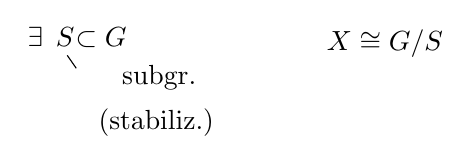
\begin{tikzpicture}[x=1mm,y=1mm,every node/.style={inner sep=0pt}]
\node[anchor=base west] (exists) at (0,13) {$\exists$};
\node[anchor=base west] (subgroup) at ([xshift=1.5mm]exists.base east) {$S$};
\node[anchor=base west] at (subgroup.base east) {$\subset G$};
\node[anchor=base west] at (38,12.6) {$X\cong G/S$};
\draw ([xshift=.25mm,yshift=-1mm]subgroup.south)--++(1.15,-1.65);
\node[anchor=base west] at (12,8.2) {subgr.};
\node[anchor=base west] at (9,2.5) {(stabiliz.)};
\end{tikzpicture}}\endgroup}
\end{GelfandAdjacentEvidence}
\begin{GelfandAdjacentEvidence}{GELFAND-P000449}{2}


\SourceFigure{GELFAND-P000449}{closing-dots}{Ten dots form a separator.
\par\smallskip\centering\color{black}
\begingroup\color{black}\GelfandFitDiagram{\begin{tikzpicture}[x=1mm,y=1mm]
\foreach \x/\y in {0/0,4/.3,9/.3,15/.4,22/.6,28/.6,33/.7,37/.5,41/.6,45/.4}
  \fill (\x,\y) circle [radius=.37mm];
\end{tikzpicture}}\endgroup}
\end{GelfandAdjacentEvidence}



\Needspace{7\baselineskip}
\begin{GelfandAdjacentEvidence}{GELFAND-P000450}{1}
\SourcePage{GELFAND-P000450}{unlabelled}
\uuline{\mbox{$25/\underline{\overline{\mathrm{IX}}}$}-72\,yr.}
\quad\uuline{Gabrielov.}

Fam. of Hodge structures over $S$ (nonsingular analyt. set)
\Unclear{GELFAND-P000450}{non-singular-word}{Two rounded strokes are joined after “б”. The reading is “неособое” (“nonsingular”).}
\end{GelfandAdjacentEvidence}
\begin{GelfandAdjacentEvidence}{GELFAND-P000450}{2}


$1)$ $\mathcal H_{\mathbb Z}$ — loc. free sheaf of $\mathbb Z$-modules of fin. type.

\sout{2)}\quad From it constr. a loc. triv. compl. bundle $H_{\mathbb C}$.
\Unclear{GELFAND-P000450}{cancelled-number}{The cancelled beginning of the line is provisionally read as “2)”.}
\end{GelfandAdjacentEvidence}
\begin{GelfandAdjacentEvidence}{GELFAND-P000450}{3}


\SourceFigure{GELFAND-P000450}{deligne-annotation}{An arrow from the complex scalar extension points to the note. The lower line of the note turns up at its left end.
\par\smallskip\centering\color{black}
\begingroup\color{black}\GelfandFitDiagram{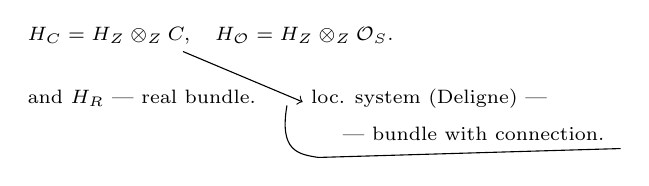
\begin{tikzpicture}[x=1mm,y=1mm,every node/.style={font=\scriptsize,inner sep=0pt,anchor=base west}]
\node (complex) at (0,16)
  {$H_{\mathbb C}=H_{\mathbb Z}\otimes_{\mathbb Z}\mathbb C,$};
\node at ([xshift=3mm]complex.base east)
  {$H_{\mathcal O}=H_{\mathbb Z}\otimes_{\mathbb Z}\mathcal O_S$.};
\node at (0,8) {and $H_{\mathbb R}$ — real bundle.};
\node (localsystem) at (36,8) {loc. system (Deligne) —};
\node (bundle) at (40,3.4) {— bundle with connection.};
\draw[->] ([xshift=-1mm,yshift=-.8mm]complex.south east)
  -- ([xshift=-1mm,yshift=.25mm]localsystem.base west);
\draw (33,7.8) .. controls (32,2) and (34.4,1.6) .. (37,1.2)
  -- ([xshift=2mm,yshift=-1mm]bundle.south east);
\end{tikzpicture}}\endgroup}
\end{GelfandAdjacentEvidence}
\begin{GelfandAdjacentEvidence}{GELFAND-P000450}{4}


$2)$ in $H_{\mathbb C}$ a decreasing filtration by holom. bundles
\[
H_{\mathbb C}=F^0\supset F^1\supset\ldots\supset F^n
\]

\SourceFigure{GELFAND-P000450}{connection-bubble}{A loop encloses the inserted “есть” (“there is”).
\par\smallskip\centering\color{black}
\begingroup\color{black}\GelfandFitDiagram{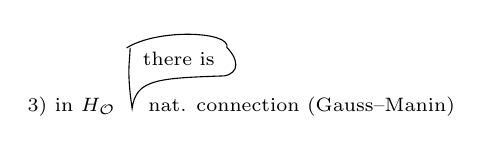
\begin{tikzpicture}[x=1mm,y=1mm,every node/.style={font=\scriptsize,inner sep=0pt,anchor=base west}]
\node (prefix) at (0,4) {$3)$ in $H_{\mathcal O}$};
\node (natural) at ([xshift=4mm]prefix.base east) {nat. connection (Gauss–Manin)};
\node (exists) at ([xshift=-.7mm,yshift=5.8mm]natural.base west) {there is};
\coordinate (tail) at ([xshift=-2mm,yshift=.4mm]natural.base west);
\draw ([xshift=-2mm,yshift=.5mm]exists.north west)
  .. controls ([xshift=2mm,yshift=3mm]exists.north west) and
              ([xshift=2mm,yshift=2.6mm]exists.north east) ..
              ([xshift=1.5mm,yshift=.55mm]exists.north east)
  .. controls ([xshift=3mm,yshift=-1mm]exists.north east) and
              ([xshift=3.1mm,yshift=-.8mm]exists.south east) ..
              ([xshift=1.2mm,yshift=-1.2mm]exists.south east)
  .. controls ([xshift=2mm,yshift=-1.5mm]exists.south west) and
              ([xshift=-.8mm,yshift=-1.6mm]exists.south west) .. (tail)
  .. controls ([xshift=-2mm,yshift=-.6mm]exists.south west) and
              ([xshift=-1.6mm,yshift=.5mm]exists.south west) ..
              ([xshift=-1.55mm,yshift=.5mm]exists.north west);
\end{tikzpicture}}\endgroup}
\end{GelfandAdjacentEvidence}
\begin{GelfandAdjacentEvidence}{GELFAND-P000450}{5}

\Unclear{GELFAND-P000450}{connection-name}{The middle letters of the first name are joined. The pair is read as “Гаусса—Манина” (“Gauss–Manin”).}
\end{GelfandAdjacentEvidence}
\begin{GelfandAdjacentEvidence}{GELFAND-P000450}{6}


\SourceFigure{GELFAND-P000450}{kernel-caption}{The note on the kernel is to the right of the formula. The mark before the dash is provisionally a comma.
\par\smallskip\centering\color{black}\scriptsize
\begin{tabular}{@{}p{.53\linewidth}@{\enspace}p{.42\linewidth}@{}}
$\nabla\colon H_{\mathcal O}\longrightarrow\Omega^1\otimes_{\mathcal O_S}H_{\mathcal O}$
& \raggedright (diff. oper. with kernel, — sect. of $H_{\mathbb C}$).\tabularnewline
\end{tabular}}
\end{GelfandAdjacentEvidence}
\begin{GelfandAdjacentEvidence}{GELFAND-P000450}{7}


(there are loc. const. sections $\mathbb Z$ — image of the sheaf $H_{\mathbb C}$)
\Unclear{GELFAND-P000450}{local-section-glyph}{The sign between “sections” and the dash is provisionally read as $\mathbb Z$. It has a loop and a long lower stroke. The exact reading is unresolved.}
\end{GelfandAdjacentEvidence}
\begin{GelfandAdjacentEvidence}{GELFAND-P000450}{8}


The connection must satisfy the cond.:
\[
\nabla(\mathcal F^p)\subset\Omega_S^1\otimes\mathcal F^{p-1}
\qquad(\mathcal F^p=F^p\otimes_{\mathbb C}\mathcal O_S)
\]

$4)$ $\psi$ — bilin., loc. const. form on $H_{\mathbb C}$, giving on restriction to $\forall$ fiber a genuine Hodge struct.

\begin{center}
\rule[.5ex]{16mm}{.35pt}\enspace$\bullet$\enspace\rule[.5ex]{19mm}{.35pt}
\end{center}
Classifying sp. of Hodge structures.

Consid.\par
\hfill\rule[.5ex]{15mm}{.35pt}\enspace$\bullet$\enspace\rule[.5ex]{15mm}{.35pt}\hspace{20mm}
\[
F=\{F^0\supset F^1\supset\ldots\supset F^n\}
\qquad\text{— flags of }\mbox{\uuline{fixed}\ \uuline{dim.}}
\]

in a fixed sp., $\mathbb C^n$ ($\dim$ can have gaps).
\begin{center}
\rule[.5ex]{16mm}{.35pt}\enspace$\bullet$\enspace\rule[.5ex]{16mm}{.35pt}
\end{center}
\SourceFigure{GELFAND-P000450}{flag-margin}{Two vertical strokes separate the right marginal note.
\par\smallskip\hfill\color{black}
\begin{tabular}{@{}||@{\enspace}l@{}}
list of $\dim$ —\\
— is given.
\end{tabular}}
\end{GelfandAdjacentEvidence}
\begin{GelfandAdjacentEvidence}{GELFAND-P000450}{9}


\underline{$D$} — sp.;

Points of the sp. \sout{\mbox{$D$}} — \underline{flags}.
\Unclear{GELFAND-P000450}{point-cancel}{The heavily overwritten sign before the dash resembles $D$. The reading of the cancelled letter is provisional.}
\end{GelfandAdjacentEvidence}
\begin{GelfandAdjacentEvidence}{GELFAND-P000450}{10}


Take a lin. sp. \uuline{\mbox{$H_{\mathbb C}$}} with a bilin. form $\psi(x,y)$
(nondeg.; skew or symm.)
\SourceFigure{GELFAND-P000450}{space-underlines}{Two lines under $H_{\mathbb C}$ sit below its lowered subscript.}
\end{GelfandAdjacentEvidence}
\begin{GelfandAdjacentEvidence}{GELFAND-P000450}{11}


$\bar D$ — set of all flags \sout{in} in $H_{\mathbb C}$
with a fixed list of $\dim$
\Unclear{GELFAND-P000450}{bar-d}{A separate stroke is visible above the heavily retraced $D$.}
\end{GelfandAdjacentEvidence}
\begin{GelfandAdjacentEvidence}{GELFAND-P000450}{12}

\Unclear{GELFAND-P000450}{bottom-cancellation}{The small cancelled sign before “в” (“in”) is provisionally read as a repeated “в”.}
\end{GelfandAdjacentEvidence}



\Needspace{7\baselineskip}
\begin{GelfandAdjacentEvidence}{GELFAND-P000451}{1}
\SourcePage{GELFAND-P000451}{72}
\sout{\ldots}\quad with condition $1)$ $\psi(F^p,F^{n-p})=0$.
\Incomplete{GELFAND-P000451}{initial-cancel}{The short cancelled sign before “with” is undeciphered.}
\end{GelfandAdjacentEvidence}
\begin{GelfandAdjacentEvidence}{GELFAND-P000451}{2}

\Unclear{GELFAND-P000451}{orthogonality-exponent}{The first formula clearly reads $n-p$. The next formula separately reads $n-p+1$.}
\end{GelfandAdjacentEvidence}
\begin{GelfandAdjacentEvidence}{GELFAND-P000451}{3}


This is an algebraic subs. $\bar D$.

$\psi$ either symm. or skew-symmetric \uuline{(def)}.

\[
2)\quad F^p\oplus\bar F^{n-p+1}\cong H_{\mathbb C}
\]
\Unclear{GELFAND-P000451}{complement-sign}{The sign before $H_{\mathbb C}$ has a wave above two horizontal strokes. A slanted mark joins the lower strokes. The reading $\cong$ is provisional. The letter $H$ is heavily retraced.}
\end{GelfandAdjacentEvidence}
\begin{GelfandAdjacentEvidence}{GELFAND-P000451}{4}

\[
H_{\mathbb Z}\subset H_{\mathbb R}\subset H_{\mathbb C}
\qquad\mbox{\uuline{also given}}
\]

The nondeg. flag determ. the grading and the Weil autom.
\[
H^{p,n-p}=F^p\cap\bar F^{n-p}
\]
Weil autom.:
\[
C\xi=i^{2p-n}\xi\quad\text{when }\xi\in H^{p,n-p}
\]
These conds. pick out in $\bar D$ the open subs. $D$.

\sout{\ldots}\qquad Another condition:\quad $\psi(x,C\bar x)>0$ when $x\ne0$.
\Incomplete{GELFAND-P000451}{condition-cancel}{Several horizontal strokes cover the earlier writing before “Another condition”. The ending has a loop and a stop. The text is unresolved.}
\end{GelfandAdjacentEvidence}
\begin{GelfandAdjacentEvidence}{GELFAND-P000451}{5}


Define on $D$ the structure of a homog. sp..

$G$ — group of all real transf. of $H_{\mathbb R}$, preserv. $\psi$
\[
\bigl(\psi(gx,gy)=\psi(x,y)\bigr).
\]
\Unclear{GELFAND-P000451}{group-equation}{The left outer parenthesis is heavily retraced. Two round closing parentheses are distinguishable on the right.}
\end{GelfandAdjacentEvidence}
\begin{GelfandAdjacentEvidence}{GELFAND-P000451}{6}


\uwave{Then \mbox{$G$} acts on \mbox{$D$}}

\SourceFigure{GELFAND-P000451}{theorem-insert}{Before $G$ is a short inscription provisionally read as “яв.” (“expl.”) and a heavily retraced sign. A $1$ is inserted in the loop above it. The beginning of the line provisionally reads $1)$.
\par\smallskip\centering\color{black}
\begingroup\color{black}\GelfandFitDiagram{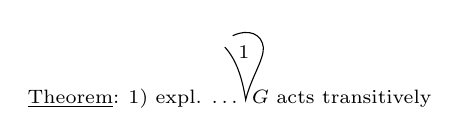
\begin{tikzpicture}[x=1mm,y=1mm,every node/.style={anchor=base west,inner sep=0pt,font=\scriptsize}]
\node (theorem) at (0,4) {\underline{Theorem}:};
\node (old) at ([xshift=1mm]theorem.base east) {$1)$ expl. \sout{\ldots}};
\node (g) at ([xshift=1.2mm]old.base east) {$G$ acts transitively};
\node at ([xshift=-1.7mm,yshift=5.7mm]g.base west) {$1$};
\coordinate (tail) at ([xshift=-.7mm,yshift=.4mm]g.base west);
\draw ([xshift=-3.35mm,yshift=7.1mm]g.base west)
  .. controls ([xshift=-1.95mm,yshift=5.6mm]g.base west) and
              ([xshift=-1.15mm,yshift=3.3mm]g.base west) .. (tail)
  .. controls ([xshift=-.05mm,yshift=3.15mm]g.base west) and
              ([xshift=1.6mm,yshift=5.45mm]g.base west) ..
              ([xshift=1.55mm,yshift=7.05mm]g.base west)
  .. controls ([xshift=1.35mm,yshift=8.75mm]g.base west) and
              ([xshift=-.25mm,yshift=9.5mm]g.base west) ..
              ([xshift=-2.35mm,yshift=8.55mm]g.base west);
\end{tikzpicture}}\endgroup}
\end{GelfandAdjacentEvidence}


$2)$ stab. Subgroup $H$ (preserv. the flag) is compact.

\underline{Proof:}\quad from explicit computation of $G$ and $H$.

$K\subset G$ — max. comp. subgroup

$G/H\longrightarrow G/K$\quad it is not holomorphic

In $G/K$ there is a compl. structure


\Needspace{7\baselineskip}
\begin{GelfandAdjacentEvidence}{GELFAND-P000452}{1}
\SourcePage{GELFAND-P000452}{unlabelled}
\underline{\sout{\ldots}}.\qquad
\rule[.5ex]{13mm}{.35pt}\enspace$\cdot$\enspace\rule[.5ex]{17mm}{.35pt}
\Incomplete{GELFAND-P000452}{title-cancel}{Closely spaced wavy strokes cover the underlined heading. A stop is visible to the right. The letters are unresolved.}
\end{GelfandAdjacentEvidence}
\begin{GelfandAdjacentEvidence}{GELFAND-P000452}{2}


\underline{Manin’s 1st lecture on \mbox{$p$}-adic numbers.}\quad (retelling)

$K$ — loc. field, (\sout{\ldots}
\Incomplete{GELFAND-P000452}{k-cancel}{After the comma are a left parenthesis and a short, heavily cancelled inscription. The right parenthesis in this line is unclear.}
\end{GelfandAdjacentEvidence}
\begin{GelfandAdjacentEvidence}{GELFAND-P000452}{3}

(fin. ext. of the $p$-adic numbers)\quad
\sout{or form. pow. series over}\par\hspace{23mm}\sout{a fin. field})
\Incomplete{GELFAND-P000452}{parent-cancel-full}{The cancelled lines are provisionally read as “or form. pow. series over” and “a fin. field”. The closing parenthesis near “adic numbers” is heavily retraced.}
\end{GelfandAdjacentEvidence}
\begin{GelfandAdjacentEvidence}{GELFAND-P000452}{4}


\SourceFigure{GELFAND-P000452}{maximal-ideal-annotation}{A short vertical stroke connects $m$ with the label below.
\par\smallskip\centering\color{black}
\begingroup\color{black}\GelfandFitDiagram{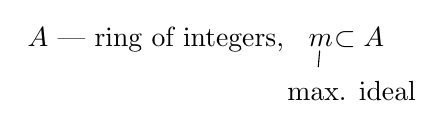
\begin{tikzpicture}[x=1mm,y=1mm,every node/.style={anchor=base west,inner sep=0pt}]
\node (ring) at (0,9) {$A$ — ring of integers,};
\node (ideal) at ([xshift=3mm]ring.base east) {$m$};
\node at (ideal.base east) {$\subset A$};
\draw ([xshift=-.15mm,yshift=-.4mm]ideal.south) -- ++(-.18,-2.1);
\node at ([xshift=-2.7mm,yshift=-6.8mm]ideal.base west) {max. ideal};
\end{tikzpicture}}\endgroup}
\end{GelfandAdjacentEvidence}
\begin{GelfandAdjacentEvidence}{GELFAND-P000452}{5}


$P^1(K)$ — proj. line.
\[
\begin{aligned}
G &= \text{its motions}\quad
   \left\{z\longrightarrow\frac{az+b}{cz+d}\ \middle|\ 
     a,b,c,d\in K,\ \det\ne0\right\}=\\
  &= \operatorname{GL}(2,K)/K^*
\end{aligned}
\]
\Unclear{GELFAND-P000452}{mobius-det}{The notation before the right brace reads $\det\ne0$. The sign is heavily retraced. Two horizontal strokes immediately after the brace read as $=$. The next line also starts with $=$.}
\end{GelfandAdjacentEvidence}
\begin{GelfandAdjacentEvidence}{GELFAND-P000452}{6}


$U\subset G$;\quad $U=\operatorname{GL}(2,A)/A^*$.

Constr. $G/U$ — graph $\Delta$ — analog of the Lobachevsky pl..

\underline{Def.}: a lattice in $K^2$ — a free $A$-module with 2 gen.
\[
L=Ae_1\oplus Ae_2.
\]
\underline{Lemma}. If $L_1$ and $L_2$ — 2 latt.,
then $\exists$ a basis $e_1,e_2$ in $K^2$, such that
\[
\begin{gathered}
L_1=Ae_1\oplus Ae_2;\qquad L_2=m^{\nu_1}e_1\oplus m^{\nu_2}e_2=\\
{}=A\pi^{\nu_1}e_1\oplus A\pi^{\nu_2}e_2
\end{gathered}
\]

\hfill($\pi$ — generator [?] of the max. ideal)
\Unclear{GELFAND-P000452}{ideal-symbol-tight}{A looped mark with a lengthwise stroke stands between “generator” and “max.” in the Russian. Its reading is unresolved.}
\end{GelfandAdjacentEvidence}
\begin{GelfandAdjacentEvidence}{GELFAND-P000452}{7}


\SourceFigure{GELFAND-P000452}{integer-note}{The inscription $\nu_1,\nu_2\in\mathbb Z$ sits at the right between the two parenthetical lines.
\par\smallskip\color{black}
(analog. to the lin. alg. theor. on simult. reduction)\hfill
\raisebox{1ex}{$\nu_1,\nu_2\in\mathbb Z$}}
\end{GelfandAdjacentEvidence}
\begin{GelfandAdjacentEvidence}{GELFAND-P000452}{8}


\underline{Def.}\quad $L_1\sim L_2$, if
\underline{$L_1=\alpha L_2$}, where $\alpha\in K^*$.

\begin{center}
\rule[.5ex]{17mm}{.35pt}\enspace$\cdot$\enspace\rule[.5ex]{19mm}{.35pt}
\end{center}
There is an analog of distance — as in symm. sp.. \sout{\ldots}\ — see \underline{A. Weil}
\Incomplete{GELFAND-P000452}{sim-margin-cancel}{The small sign before the dash is cancelled. Its reading is unresolved.}
\end{GelfandAdjacentEvidence}
\begin{GelfandAdjacentEvidence}{GELFAND-P000452}{9}


\begin{center}
\rule[.5ex]{17mm}{.35pt}\enspace$\cdot$\enspace\rule[.5ex]{19mm}{.35pt}
\end{center}
Vertices of graph $\Delta^{(0)}_{\text{\sout{\ldots}}}$ — equiv. classes of lattices
\Incomplete{GELFAND-P000452}{dimension-glyph}{A small cancelled sign appears below and to the right of the first $\Delta$. Its reading is unresolved. Above it is $(0)$.}
\end{GelfandAdjacentEvidence}


$G$ acts on $\Delta^{(0)}$.


\Needspace{7\baselineskip}
\begin{GelfandAdjacentEvidence}{GELFAND-P000453}{1}
\SourcePage{GELFAND-P000453}{73}
\SourceFigure{GELFAND-P000453}{class-arrow}{The arrow by $\Delta^{(0)}$ points down and left toward the first entry.
\par\smallskip\centering\color{black}
\begingroup\color{black}\GelfandFitDiagram{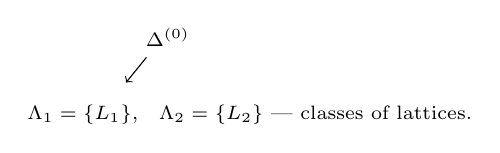
\begin{tikzpicture}[x=1mm,y=1mm,every node/.style={inner sep=0pt,anchor=base west,font=\scriptsize}]
\node (first) at (0,1) {$\Lambda_1=\{L_1\},$};
\node at ([xshift=2.5mm]first.base east) {$\Lambda_2=\{L_2\}$ — classes of lattices.};
\node at (15,10.3) {$\Delta^{(0)}$};
\draw[->] (15.15,8.9) -- (12.55,5.7);
\end{tikzpicture}}\endgroup}
\end{GelfandAdjacentEvidence}
\begin{GelfandAdjacentEvidence}{GELFAND-P000453}{2}


\SourceFigure{GELFAND-P000453}{inclusion-and-residue}{The frame under $L_2\subset L_1$ is open at the top. Two vertical strokes set off the residue field on the right. The left stroke of $F$ is doubled.
\par\smallskip\centering\color{black}
\begingroup\color{black}\GelfandFitDiagram{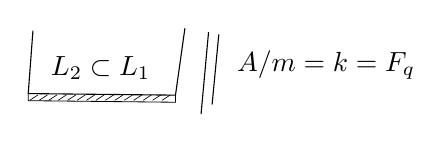
\begin{tikzpicture}[x=1mm,y=1mm]
\node[inner sep=0pt] at (11,7.8) {$L_2\subset L_1$};
\draw (2.4,12.6)--(1.8,4.6)--(20.5,4.4)--(21.7,12.9);
\draw[line width=.3pt] (1.8,4.6)--(1.8,3.7)--(20.5,3.5)--(20.5,4.4);
\foreach \x in {2.0,3.2,...,19.4}{\draw[line width=.24pt] (\x,3.75)--++(1.05,.68);}
\draw (24.7,12.4)--(23.75,2) (26,12.1)--(25.15,3.2);
\node[anchor=west,inner sep=0pt] at (28.25,8.2) {$A/m=k=\mathbb F_q$};
\end{tikzpicture}}\endgroup}
\end{GelfandAdjacentEvidence}
\begin{GelfandAdjacentEvidence}{GELFAND-P000453}{3}


\[
\begin{gathered}
L_1=Ae_1\oplus Ae_2\\
L_2=Ae_1\oplus A\pi^\nu e_2
\end{gathered}
\]
— thus choose the representatives,\quad \uuline{\mbox{$\nu\ge0$}.}
\Unclear{GELFAND-P000453}{representative-word}{The end of the last word is faint. The reading is “представители” (“representatives”).}
\end{GelfandAdjacentEvidence}
\begin{GelfandAdjacentEvidence}{GELFAND-P000453}{4}


$\nu$ is called distance\qquad \uuline{\mbox{$\nu=d(\Lambda_1,\Lambda_2)$}.}

\SourceFigure{GELFAND-P000453}{quotient-cancel}{Three strokes frame the formula below and at the sides. The inscription after the equals sign is heavily cancelled. Its reading is unresolved.
\par\smallskip\centering\color{black}
\begingroup\color{black}\GelfandFitDiagram{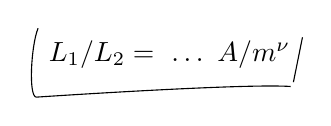
\begin{tikzpicture}[x=1mm,y=1mm]
\node[inner sep=0pt,anchor=base west] (quotient) at (3,5.1)
  {$L_1/L_2={}$ \sout{\ldots}\ $A/m^\nu$};
\path ([yshift=-2.25mm]quotient.south east) coordinate (right);
\draw (1.7,9.3) .. controls (.8,7.1) and (.45,.5) .. (1.5,.55)
  .. controls (9,1.05) and ([xshift=-5mm,yshift=.35mm]right) .. (right);
\draw ([xshift=.35mm,yshift=.55mm]right)--++(1.15,5.7);
\end{tikzpicture}}\endgroup}
\end{GelfandAdjacentEvidence}
\begin{GelfandAdjacentEvidence}{GELFAND-P000453}{5}


\underline{Thm.}\quad This is a corr. def. and is a \underline{distance}.
\begin{center}
\rule[.5ex]{14mm}{.35pt}\enspace$\cdot$\enspace\rule[.5ex]{21mm}{.35pt}
\end{center}

\uuline{Variant:}
\[
L_1/L_2\simeq A/\pi^{\nu_1}A\oplus A/\pi^{\nu_2}A
\]
\Unclear{GELFAND-P000453}{variant-sign}{A single straight stroke lies under the wave. It is set as $\simeq$.}
\end{GelfandAdjacentEvidence}
\begin{GelfandAdjacentEvidence}{GELFAND-P000453}{6}

\[
d(\Lambda_1,\Lambda_2)=|\nu_1-\nu_2|
\]

$\Lambda_1,\Lambda_2$ — neighbors in $\Lambda^0$, if $d(\Lambda',\Lambda^2)=1$.
\Unclear{GELFAND-P000453}{neighbor-notation}{The set has a $\Lambda$ with a small raised circle. In the arguments of $d$, a raised stroke follows the first $\Lambda$ and a raised $2$ follows the second.}
\end{GelfandAdjacentEvidence}
\begin{GelfandAdjacentEvidence}{GELFAND-P000453}{7}


Join them by an edge. We obtain a graph $\Delta$.

\underline{Theorem}:\quad $\Delta$ — a tree (conn. graph without cycles),
and from $\forall$ vertex there issue exactly $q+1$ edges

$\Delta$ is the Lobachevsky pl. — there acts $G$ etc.

\SourceFigure{GELFAND-P000453}{disk-figure}{The outer boundary has a gap at the upper right. The inner arcs and chain follow the visible strokes. A fine mark by the lower left arc resembles an oval. Some joins in the upper right remain uncertain.
\par\smallskip\centering\color{black}
\begingroup\color{black}\GelfandFitDiagram{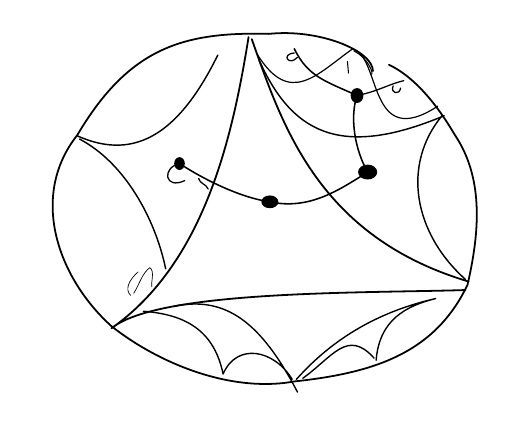
\begin{tikzpicture}[x=.135mm,y=-.135mm,line cap=round,line join=round]
% The outline is broken near the top right, as in the manuscript.
\draw[line width=.64pt] (325,52)
  .. controls (325,33) and (275,12) .. (227,17)
  .. controls (148,15) and (96,29) .. (47,112)
  .. controls (1,170) and (29,247) .. (79,292)
  .. controls (122,326) and (190,355) .. (251,344)
  .. controls (325,336) and (383,318) .. (414,253)
  .. controls (424,209) and (431,155) .. (402,112)
  .. controls (382,78) and (361,56) .. (340,46);
% Main arcs and boundary wedges.
\draw[line width=.65pt] (208,20) .. controls (193,113) and (167,232) .. (79,294)
  .. controls (123,258) and (314,261) .. (412,258);
\draw[line width=.65pt] (211,22) .. controls (240,104) and (274,208) .. (415,250);
\draw[line width=.52pt] (47,113) .. controls (103,138) and (144,108) .. (179,37)
  (49,116) .. controls (91,138) and (120,190) .. (130,238);
\draw[line width=.52pt] (218,42) .. controls (248,108) and (292,136) .. (392,94)
  (390,94) .. controls (352,140) and (363,204) .. (412,248);
\draw[line width=.43pt] (216,36) .. controls (247,86) and (272,55) .. (306,31)
  .. controls (333,39) and (320,128) .. (386,85);
\draw[line width=.37pt] (307,33) .. controls (320,39) and (327,56) .. (323,55)
  (301,43)--(302,54);
\draw[line width=.5pt] (109,278) .. controls (151,281) and (176,298) .. (184,337)
  .. controls (197,307) and (232,314) .. (249,342)
  (139,273) .. controls (186,264) and (219,287) .. (254,354)
  (253,342) .. controls (285,306) and (327,279) .. (384,266)
  .. controls (356,273) and (331,286) .. (328,324)
  (259,341) .. controls (287,321) and (301,294) .. (326,322);
% Inner chain, its short branches, and the separate fine lower-left mark.
\draw[line width=.56pt] (143,139) .. controls (166,154) and (200,171) .. (228,175)
  .. controls (265,183) and (293,164) .. (320,147)
  .. controls (308,126) and (303,96) .. (310,75)
  .. controls (282,62) and (264,58) .. (251,31);
\draw[line width=.46pt] (310,75) .. controls (330,71) and (338,65) .. (354,61)
  (143,139) .. controls (126,143) and (129,164) .. (148,155)
  (161,153) .. controls (162,158) and (168,158) .. (170,163)
  (251,35) .. controls (238,36) and (246,48) .. (254,39)
  (344,66) .. controls (341,73) and (350,75) .. (351,68);
\fill (143,139) ellipse [x radius=5,y radius=6];
\fill (228,175) ellipse [x radius=8,y radius=6];
\fill (320,147) ellipse [x radius=9,y radius=7];
\fill (310,75) ellipse [x radius=6,y radius=7];
\draw[line width=.25pt] (97,263) .. controls (91,257) and (96,248) .. (104,241)
  (100,261) .. controls (105,253) and (108,242) .. (115,237)
  .. controls (120,240) and (116,250) .. (117,255);
\end{tikzpicture}}\endgroup}
\end{GelfandAdjacentEvidence}


\begin{center}
\rule[.5ex]{18mm}{.35pt}\enspace$\bullet$\enspace\rule[.5ex]{21mm}{.35pt}
\end{center}


\Needspace{7\baselineskip}
\begin{GelfandAdjacentEvidence}{GELFAND-P000454}{1}
\SourcePage{GELFAND-P000454}{unlabelled}
\uuline{D. Kazhdan}.\quad Tate's art., Matematika, \underline{$13:2$, §$3$}.

(on the field $\mathbb C_p$ — completion of the alg. closure $\overline{\mathbb Q}_p$ or
$\mathbb Q_p$ — $p$-adic numbers)
\Unclear{GELFAND-P000454}{q-p-link-word}{The connecting word reads “or.”}
\end{GelfandAdjacentEvidence}
\begin{GelfandAdjacentEvidence}{GELFAND-P000454}{2}


\begin{center}
\rule[.5ex]{14mm}{.35pt}\enspace$\cdot$\enspace\rule[.5ex]{21mm}{.35pt}
\end{center}

$K$ — finite ext. of the field $\mathbb Q_p$.

\SourceFigure{GELFAND-P000454}{vertical-ring}{There is a curved stroke between the two entries. Its meaning is uncertain. Two short vertical strokes sit below the second entry.
\par\smallskip\centering\color{black}
\begingroup\color{black}\GelfandFitDiagram{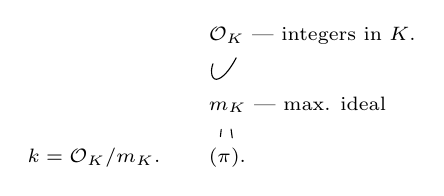
\begin{tikzpicture}[x=1mm,y=1mm,line cap=round,every node/.style={inner sep=0pt,anchor=base west,font=\scriptsize}]
\node at (0,1) {$k=\mathcal O_K/m_K$.};
\node at (23,16.5) {$\mathcal O_K$ — integers in $K$.};
\draw (23.6,13.6) .. controls (23.2,12.55) and (23.45,11.3) .. (24.35,11.7)
  .. controls (25.15,12.05) and (25.95,13.2) .. (26.55,14.35);
\node at (23,7.7) {$m_K$ — max. ideal};
\draw (24.65,5.25)--(24.55,4.35) (25.9,5.3)--(26.05,4.2);
\node at (23,1) {$(\pi)$.};
\end{tikzpicture}}\endgroup}
\end{GelfandAdjacentEvidence}
\begin{GelfandAdjacentEvidence}{GELFAND-P000454}{3}


$L$ — finite ext. of $K$, \sout{\ldots} $\mathcal O_L$ — integers in it

\Unclear{GELFAND-P000454}{ol-cancel}{The crossed-out marks before $\mathcal O_L$ are illegible.}
\end{GelfandAdjacentEvidence}
\begin{GelfandAdjacentEvidence}{GELFAND-P000454}{4}


$m_L=(\tau)$,\quad $\ell=\mathcal O_L/m_L$,
\[
G=\operatorname{Gal}(L:K)
\]
Introduce a filtration in $G$ and prove that $G$ is solvable.

On $L$ and $K$ \sout{\ldots} define a norm so that
$|\pi|=(\operatorname{Card}k)^{-1}$
\Unclear{GELFAND-P000454}{norm-cancel}{A crossed-out sign sits between $K$ and “define.” Its reading is uncertain.}
\end{GelfandAdjacentEvidence}
\begin{GelfandAdjacentEvidence}{GELFAND-P000454}{5}


\uuline{Def.}\quad \sout{\ldots}.
\Incomplete{GELFAND-P000454}{def-cancel}{A short entry is crossed out after “Def.” Its reading is uncertain.}

\[
g\in G_i\Longleftrightarrow \forall x\in \mathcal O_L\quad x^g-x\in m_L^i
\]
\[
G=G_0\supset G_1\supset\ldots\supset G_n=\{e\}.
\]
\end{GelfandAdjacentEvidence}
\begin{GelfandAdjacentEvidence}{GELFAND-P000454}{6}
$G_i$ — normal subgroup in $G$.

\underline{Theorem:}\quad $G_i/G_{i+1}$ — ab. group

$1)$ \underline{$i=0$.}\qquad
$G\overset{\varphi}{\longrightarrow}\operatorname{Gal}(\ell:k)$
(natural map)

\underline{Construction of $\varphi$:}\quad $\bar x\in\ell,\ g\in G$
\[
x\in L\qquad \bar x^g\overset{\mathrm{def}}{=}\overline{x^g}
\]
\Unclear{GELFAND-P000454}{residue-representative}{The manuscript reads $x\in L$.}
\end{GelfandAdjacentEvidence}
\begin{GelfandAdjacentEvidence}{GELFAND-P000454}{7}


$g\in\ker\varphi\Longleftrightarrow \bar x\in\ell,\ \bar x^g=\bar x$,
i.e. $\bar x^g-\bar x=0$, i.e.
\Unclear{GELFAND-P000454}{kernel-quantifier}{The equivalence sign is followed by $\bar x\in\ell$. No explicit quantifier is visible.}
\end{GelfandAdjacentEvidence}



\Needspace{7\baselineskip}
\begin{GelfandAdjacentEvidence}{GELFAND-P000455}{1}
\SourcePage{GELFAND-P000455}{74}
\sout{i.e. \ldots}\qquad $x^g-x\in m_L$, i.e. $g\in G_1$.
\Unclear{GELFAND-P000455}{top-old-fragment}{The start of the crossed-out entry provisionally reads “i.e.”.}
\end{GelfandAdjacentEvidence}
\begin{GelfandAdjacentEvidence}{GELFAND-P000455}{2}

\Incomplete{GELFAND-P000455}{top-cancelled}{The remainder of the crossed-out entry is illegible.}
\end{GelfandAdjacentEvidence}
\begin{GelfandAdjacentEvidence}{GELFAND-P000455}{3}


\[
0\longrightarrow G_0/G_1\xrightarrow{\varphi}\operatorname{Gal}(\ell:k)
\]
\underline{Exercise:}\quad $\varphi$ — an isomorphism.

$2)$\quad $G_1/G_2$ — $?$
\Unclear{GELFAND-P000455}{quotient-question}{A question mark follows the dash.}
\end{GelfandAdjacentEvidence}
\begin{GelfandAdjacentEvidence}{GELFAND-P000455}{4}


\[
G_1\xrightarrow{\psi_1}\ell^*
\qquad
g\mathrel{\sim\!\longrightarrow}\overline{\tau^g/\tau}
\qquad\text{(indep. of the choice of $\tau$)}
\]
\Unclear{GELFAND-P000455}{ramification-label}{The first arrow is labelled $\psi_1$.}
\end{GelfandAdjacentEvidence}
\begin{GelfandAdjacentEvidence}{GELFAND-P000455}{5}


Its kernel is $G_2$.
\Unclear{GELFAND-P000455}{kernel-pronoun}{The word following “kernel” reads «его» (“its”).}
\end{GelfandAdjacentEvidence}
\begin{GelfandAdjacentEvidence}{GELFAND-P000455}{6}


\[
\begin{aligned}
G_i/G_{i+1}&\longrightarrow\ell^+
   \qquad\text{(addit. group of the field $\ell$).}\\
g&\xrightarrow{\psi_i}
\overline{\left(\frac{\tau^g/\tau-1}{\tau^{i-1}}\right)}
\end{aligned}
\]
\Unclear{GELFAND-P000455}{higher-label}{The arrow from $g$ is labelled $\psi_i$.}
\end{GelfandAdjacentEvidence}
\begin{GelfandAdjacentEvidence}{GELFAND-P000455}{7}

\underline{Thm.}\quad $G_{i+1}=\operatorname{Ker}\psi_i$.
\Unclear{GELFAND-P000455}{kernel-domain}{The domain on the upper line is written $G_i/G_{i+1}$. The line below has $G_{i+1}=\operatorname{Ker}\psi_i$.}
\end{GelfandAdjacentEvidence}
\begin{GelfandAdjacentEvidence}{GELFAND-P000455}{8}


$G_1$ is called the inertia subgroup of the Galois grp.

Unramified extension $\underset{\mathrm{def}}{\Longleftrightarrow} G_1=\{e\}$;

weakly ramif. $G_2=\{e\}$.
\Unclear{GELFAND-P000455}{weak-word}{The second letter is overwritten. The abbreviation reads «слаборазветвл.» (“weakly ramif.”).}
\end{GelfandAdjacentEvidence}
\begin{GelfandAdjacentEvidence}{GELFAND-P000455}{9}


purely ramified $G_0=G_1$
\Unclear{GELFAND-P000455}{last-subscript}{The last subscript is overwritten. It provisionally reads $1$.}
\end{GelfandAdjacentEvidence}


\begin{center}
\rule[.5ex]{25mm}{.35pt}\enspace$\cdot$\enspace\rule[.5ex]{35mm}{.35pt}
\end{center}


\Needspace{7\baselineskip}
\begin{GelfandAdjacentEvidence}{GELFAND-P000456}{1}
\SourcePage{GELFAND-P000456}{unlabelled}
\underline{The seminar will start at \mbox{$18^{\underline{00}}$}.}

\uuline{2/X-72.}\qquad \underline{A. Gabrielov.}

$S$ — compl. analytic set

$H_{\mathbb Z}$ — loc. free $\mathbb Z$-sheaf

($\mathbb Z$ — const. sheaf; a section over a conn. region is a const. integer;
$H_{\mathbb Z}$ — loc. free sheaf of $\mathbb Z$-modules.
\Unclear{GELFAND-P000456}{modules-old}{Overlapping strokes follow “modules.” Their reading is uncertain.}
\end{GelfandAdjacentEvidence}
\begin{GelfandAdjacentEvidence}{GELFAND-P000456}{2}

At $\forall$ point $\exists$ nbhd.,
in which it is isom. to $\mathbb Z\oplus\cdots\oplus\mathbb Z$).

\sout{\mbox{$H$}\ldots}\quad
\Unclear{GELFAND-P000456}{start-old-fragment}{The first crossed-out sign provisionally reads $H$.}
\end{GelfandAdjacentEvidence}
\begin{GelfandAdjacentEvidence}{GELFAND-P000456}{3}

\Incomplete{GELFAND-P000456}{start-cancelled}{The rest of the short entry before the parenthesis is illegible.}
\end{GelfandAdjacentEvidence}
\begin{GelfandAdjacentEvidence}{GELFAND-P000456}{4}

($\mathbb Z$-sheaf assoc. with the presheaf which \sout{\ldots}\ \sout{\ldots}
\par\noindent\hspace*{2em}$F(U)=\mathbb Z$).
\Incomplete{GELFAND-P000456}{presheaf-full-cancel}{Two entries after “which” are crossed out. Below them is $F(U)=\mathbb Z$.}
\end{GelfandAdjacentEvidence}
\begin{GelfandAdjacentEvidence}{GELFAND-P000456}{5}


The space is loc. connected $\Rightarrow$ fiber $=\mathbb Z$.

The space of the sheaf $\mathbb Z$ is homeom. to $S\times\mathbb Z$.

Loc. $\left.H_{\mathbb Z}\right|_U\simeq U\times\mathbb Z^n$
\[
\Gamma(U,H_{\mathbb Z})\cong\mathbb Z^n
\]
$S$ is connected $\Rightarrow$ $n$ is the same everywhere.

Cover by neighborhoods and fix isomorphisms over the neighborhoods\\
\hspace*{2em}(up to $GL(n,\mathbb Z)$)

\SourceFigure{GELFAND-P000456}{overlap-sketch}{Two overlapping ovals with four strokes in their intersection. There is an angular mark on the left arc.
\par\smallskip\centering\color{black}
\begingroup\color{black}\GelfandFitDiagram{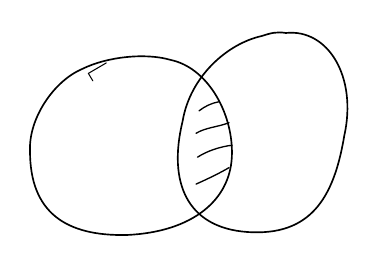
\begin{tikzpicture}[x=.19mm,y=-.19mm,line cap=round,line join=round]
\draw[line width=.6pt] (54,35)
  .. controls (35,43) and (18,68) .. (19,90)
  .. controls (19,131) and (43,147) .. (84,146)
  .. controls (127,144) and (154,123) .. (154,91)
  .. controls (154,63) and (137,34) .. (113,29)
  .. controls (96,24) and (70,27) .. (54,35);
\draw[line width=.6pt] (174,13)
  .. controls (151,18) and (126,40) .. (121,70)
  .. controls (111,111) and (124,141) .. (164,144)
  .. controls (206,147) and (222,122) .. (229,80)
  .. controls (238,40) and (218,8) .. (190,11)
  .. controls (184,10) and (180,11) .. (174,13);
\draw[line width=.38pt] (70,31)--(58,38)--(61,43);
\draw[line width=.48pt]
 (132,63)..controls(136,60)and(140,58)..(145,57)
 (130,78)..controls(137,74)and(144,74)..(152,71)
 (131,94)..controls(137,90)and(146,87)..(154,86)
 (130,112)..controls(139,108)and(147,104)..(152,101);
\end{tikzpicture}}\endgroup}
\end{GelfandAdjacentEvidence}
\begin{GelfandAdjacentEvidence}{GELFAND-P000456}{6}


transition functions from $GL(n,\mathbb Z)$.

One can construct a \uwave{loc. triv.} bundle with such transition functions.

\SourceFigure{GELFAND-P000456}{complex-bundle-link}{A slanted stroke links $H_{\mathbb C}$ to the caption.
\par\smallskip\centering\color{black}
\begingroup\color{black}\GelfandFitDiagram{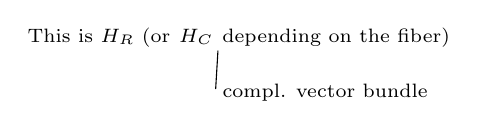
\begin{tikzpicture}[x=1mm,y=1mm,line cap=round,every node/.style={inner sep=0pt,anchor=base west,font=\scriptsize}]
\node (first) at (0,8) {This is $H_{\mathbb R}$ (or};
\node (hc) at ([xshift=1mm]first.base east) {$H_{\mathbb C}$};
\node at ([xshift=1mm]hc.base east) {depending on the fiber)};
\node (label) at ([xshift=5.5mm,yshift=-7mm]hc.base west) {compl. vector bundle};
\draw ([xshift=.5mm,yshift=-1.1mm]hc.base east)--([xshift=-.8mm,yshift=1.1mm]label.base west);
\end{tikzpicture}}\endgroup}
\end{GelfandAdjacentEvidence}
\begin{GelfandAdjacentEvidence}{GELFAND-P000456}{7}


\SourceFigure{GELFAND-P000456}{holomorphic-sections-link}{A vertical stroke leads to the wavy-underlined caption. The rectangle at right is crossed out.
\par\smallskip\centering\color{black}
\begingroup\color{black}\GelfandFitDiagram{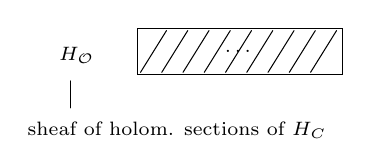
\begin{tikzpicture}[x=1mm,y=1mm,line cap=round,every node/.style={inner sep=0pt,font=\scriptsize}]
\node[anchor=base west] at (4,10.5) {$H_{\mathcal O}$};
\draw (14,8.7) rectangle (40,14.6);
\foreach \x in {14.4,17.1,19.8,22.5,25.2,27.9,30.6,33.3,36.0}
  \draw[line width=.37pt] (\x,9) -- ++(3.3,5.3);
\node at (27,11.65) {\sout{\ldots}};
\draw (5.5,7.9)--(5.5,4.5);
\node[anchor=base west] at (0,1) {\uwave{sheaf of holom. sections of \mbox{$H_{\mathbb C}$}}};
\end{tikzpicture}}\endgroup}
\end{GelfandAdjacentEvidence}
\begin{GelfandAdjacentEvidence}{GELFAND-P000456}{8}

\Unclear{GELFAND-P000456}{o-old-fragment}{The crossed-out entry may start with $H$ and a subscript.}
\end{GelfandAdjacentEvidence}
\begin{GelfandAdjacentEvidence}{GELFAND-P000456}{9}

\Incomplete{GELFAND-P000456}{o-cancelled}{The crossed-out entry inside the rectangle is illegible.}
\end{GelfandAdjacentEvidence}

\[
H_{\mathcal O}=H_{\mathbb Z}\otimes_{\mathbb Z}\mathcal O_S.
\]
There is a natural connection (Gauss–Manin)
\[
\nabla\colon H_{\mathcal O}\longrightarrow
\Omega_S^1\otimes_{\mathcal O_S}H_{\mathcal O}
\qquad\text{($\mathbb C$-lin. homom.)}
\]
$\Omega_S^1$ — holom. diff. forms of order $1$


\Needspace{7\baselineskip}
\begin{GelfandAdjacentEvidence}{GELFAND-P000457}{1}
\SourcePage{GELFAND-P000457}{75}
\underline{def. of connection.}

$1.$ $\mathbb C$-linearity.

$2.$ $\varphi\in\mathcal O_{S,s}$ (germs), $f\in H_{\mathcal O,s}\Rightarrow$
\[
\Rightarrow\nabla(\varphi f)=\varphi\nabla f+d\varphi\otimes f
\]
\underline{Our connection.}

Take a loc. trivialization\\
and a basis of const. sections (bundle $H_{\mathbb Z}$) $u_i$
\[
f=\sum\varphi_i u_i,\qquad\varphi_i\in\mathcal O_S
\]
Then
\[
\nabla f=\sum d\varphi_i\otimes u_i
\]
This def. is well-defined and satisfies all the axioms.

The curvature of this connection equals $0$.
\Unclear{GELFAND-P000457}{curvature-sign}{The last sign reads $0$.}
\end{GelfandAdjacentEvidence}
\begin{GelfandAdjacentEvidence}{GELFAND-P000457}{2}


\underline{Requirement on the G.-M. connection}\quad
(\underline{or on the} \sout{\ldots}\ \underline{filtration})
\[
\nabla(\mathcal F^p)\subset\Omega_S^1\otimes\mathcal F^{p-1}.
\]
\hfill(Griffiths)\par
\Unclear{GELFAND-P000457}{filter-old}{The crossed-out sign after “or on the” is illegible.}
\end{GelfandAdjacentEvidence}
\begin{GelfandAdjacentEvidence}{GELFAND-P000457}{3}


(Given a filtration $H_{\mathbb C}=F^0\supset F^1\supset\cdots$)\\
\hspace*{4em}by holom. subbundles

$\mathcal F^p$ — sheaves of sections of $F^p$

\begin{center}
\rule[.5ex]{15mm}{.35pt}\enspace$\cdot$\enspace\rule[.5ex]{22mm}{.35pt}
\end{center}

\uwave{There is a loc. constant bilin. form \mbox{$\psi(x,y)$} on \mbox{$H_{\mathbb C}$}}
\Unclear{GELFAND-P000457}{form-letter}{The letter before $(x,y)$ reads $\psi$.}
\end{GelfandAdjacentEvidence}
\begin{GelfandAdjacentEvidence}{GELFAND-P000457}{4}


\sout{\ldots}
\Incomplete{GELFAND-P000457}{mid-cancelled}{The short crossed-out entry before “and” is illegible.}
\end{GelfandAdjacentEvidence}
\begin{GelfandAdjacentEvidence}{GELFAND-P000457}{5}

and at $\forall$ point $s\in S$ this is a Hodge structure.

\begin{center}
\rule[.5ex]{15mm}{.35pt}\enspace$\cdot$\enspace\rule[.5ex]{22mm}{.35pt}
\end{center}

Let $0\le p\le n$,\quad $k_p\ge k_{p+1}$ — a seq. of numbers
\[
k_0\ge k_1\ge\cdots\ge k_n.
\]
$Z$ — space with elem. $F=\{F^0\supset F^1\supset\cdots\supset F^n\}$,\\
where $\dim F^p=k_p$.
\Unclear{GELFAND-P000457}{dimension-sup}{The superscript $p$ on $F$ is overwritten.}
\end{GelfandAdjacentEvidence}


This is a proj. alg. set.


\Needspace{7\baselineskip}
\begin{GelfandAdjacentEvidence}{GELFAND-P000458}{1}
\SourcePage{GELFAND-P000458}{unlabelled}
\[
H_{\mathbb C}=F^0,\qquad H_{\mathbb Z}\subset H_{\mathbb R}\subset H_{\mathbb C}.
\]
Let there be on $H_{\mathbb C}$ a given bilin. form $\psi$ (nondeg.),
\Unclear{GELFAND-P000458}{first-form}{The sign after “form” reads $\psi$.}
\end{GelfandAdjacentEvidence}
\begin{GelfandAdjacentEvidence}{GELFAND-P000458}{2}

symm. for odd $n$ and skew for even $n$; integral
\Unclear{GELFAND-P000458}{parity-statement}{The manuscript reads “symm. for odd $n$ and skew for even $n$.”}
\end{GelfandAdjacentEvidence}
\begin{GelfandAdjacentEvidence}{GELFAND-P000458}{3}


$\overline D$ — subset in $Z$ of those flags for which
\SourceFigure{GELFAND-P000458}{orthogonality-bracket}{A line encloses the formula from below and at both sides.
\par\smallskip\centering\color{black}
\begingroup\color{black}\GelfandFitDiagram{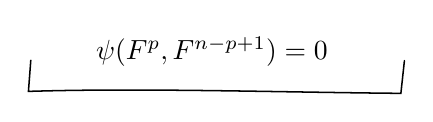
\begin{tikzpicture}[x=1mm,y=1mm,line cap=round]
\node at (25,6.4) {$\psi(F^p,F^{n-p+1})=0$};
\draw[line width=.55pt] (2,5.3)--(1.7,1.35)
  .. controls (16,1.8) and (33,1.25) .. (49,1.1)--(49.45,5.25);
\end{tikzpicture}}\endgroup}
\end{GelfandAdjacentEvidence}
\begin{GelfandAdjacentEvidence}{GELFAND-P000458}{4}


\noindent\rule{\linewidth}{.35pt}

\underline{Add. cond.}\\
\underline{on the flags}\quad $1)\quad F^p\oplus\overline{F^{n-p+1}}\cong H_{\mathbb C}$
\Unclear{GELFAND-P000458}{sum-formula}{The end of the exponent $n-p+1$ is overwritten beside the sign $\cong$.}
\end{GelfandAdjacentEvidence}
\begin{GelfandAdjacentEvidence}{GELFAND-P000458}{5}


$2)$ From it are constr. the grading and the Weil autom. $C$ and then
\[
\psi(x,C\bar y)\quad\text{pos. def. Herm. form on $H_{\mathbb C}$.}
\]
\Unclear{GELFAND-P000458}{weil-link-full}{After $C$ the manuscript reads «и тогда» (“and then”).}
\end{GelfandAdjacentEvidence}
\begin{GelfandAdjacentEvidence}{GELFAND-P000458}{6}


These conditions single out $\underset{\text{(open).}}{D}\subset\overline D$.

$D$ is called the classify. space of Hodge structures.

Depends on the set of dimensions and the form $\psi$.

\underline{Next time}: homogeneity.

grp. of the compl. space $H_{\mathbb C}$, preserv. $\psi$, transit. on $\overline D$

Conn. comp. \(\vphantom{G}_{1}\) grp. of the real space $H_{\mathbb R}$, preserv. $\psi$, transit. on $D$
\Unclear{GELFAND-P000458}{real-prefix}{The left addition provisionally reads «Св. комп.» (“conn. comp.”) with a lowered sign resembling $1$.}
\end{GelfandAdjacentEvidence}
\begin{GelfandAdjacentEvidence}{GELFAND-P000458}{7}


\medskip\noindent\rule{\linewidth}{.35pt}

\underline{Manin’s 2nd lecture}.

\medskip\noindent\rule{\linewidth}{.35pt}

\uuline{D: Kazhdan.}\quad More on Tate’s work.
\Unclear{GELFAND-P000458}{footer-heading}{Two dots sit one above the other after the initial.}



\SourceFigure{GELFAND-P000458}{bottom-mark}{A narrow mark of several strokes crosses the divider. No definite letter or arrow is visible.
\par\smallskip\centering\color{black}
\begingroup\color{black}\GelfandFitDiagram{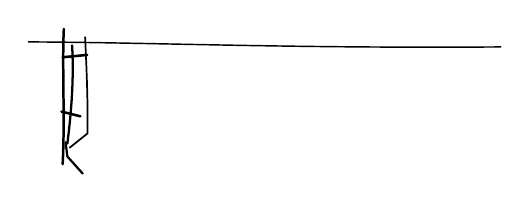
\begin{tikzpicture}[x=.75mm,y=-.75mm,line cap=round,line join=round]
\draw[line width=.52pt] (0,4.6) .. controls (22,4.7) and (43,5.7) .. (80,5.45);
\draw[line width=.9pt] (6,2.4) .. controls (5.7,8.4) and (6.2,18) .. (5.8,25.3);
\draw[line width=.82pt] (7.4,5.2) .. controls (7.8,11.9) and (7,18.6) .. (6.6,21.8);
\draw[line width=.62pt] (9.6,3.8) .. controls (9.9,9.9) and (10.1,15.8) .. (10,20.1)
 -- (7,22.5);
\draw[line width=.92pt] (5.8,7.2)--(9.95,6.8) (5.6,16.4)--(8.8,17.2);
\draw[line width=.8pt] (6.3,21.6)--(6.6,24)--(9.2,26.9);
\end{tikzpicture}}\endgroup}
\end{GelfandAdjacentEvidence}



\Needspace{10\baselineskip}
\section*{Chapter 6}

\Needspace{7\baselineskip}
\begin{GelfandAdjacentEvidence}{GELFAND-P000459}{1}
\SourcePage{GELFAND-P000459}{unlabelled}
\uuline{V. Buchstaber.}

\underline{Formal}\enspace\underline{groups}.

The def. of a formal group was given.

\SourceFigure{GELFAND-P000459}{commutative-insertion}{The abbreviation “commut.” is added in a bubble above “ring.”
\par\smallskip\centering\color{black}
\begingroup\color{black}\GelfandFitDiagram{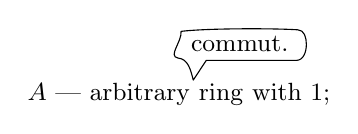
\begin{tikzpicture}[x=1mm,y=1mm,line cap=round,line join=round,every node/.style={inner sep=0pt,anchor=base west,font=\small}]
\node (start) at (0,0) {$A$ — arbitrary};
\node (ring) at ([xshift=1mm]start.base east) {ring};
\node at ([xshift=1mm]ring.base east) {with $1$;};
\node (insert) at ([xshift=-1mm,yshift=6.2mm]ring.base west) {commut.};
\draw ([xshift=-1.2mm,yshift=.6mm]insert.north west)
  .. controls ([xshift=2mm,yshift=1mm]insert.north west)
          and ([xshift=-2mm,yshift=1mm]insert.north east)
       .. ([xshift=1.1mm,yshift=.8mm]insert.north east)
  to[out=0,in=90] ([xshift=2.2mm]insert.east)
  to[out=-90,in=0] ([xshift=.9mm,yshift=-1mm]insert.south east)
  -- ([xshift=2mm,yshift=-1mm]insert.south west)
  -- ([xshift=-.65mm,yshift=.45mm]ring.north west)
  to[out=105,in=-5] ([xshift=-1.6mm,yshift=-.7mm]insert.south west)
  to[out=170,in=-85] ([xshift=-1.2mm,yshift=.6mm]insert.north west);
\end{tikzpicture}}\endgroup}
\end{GelfandAdjacentEvidence}
\begin{GelfandAdjacentEvidence}{GELFAND-P000459}{2}

\[
\sum_{i=0}^{\infty}a_i x^i,\qquad a_i\in A
\]
Form. group:
\[
F(x,y)=x+y+\sum_{i+k\ge2}a_{ik}x^iy^k
\]
— form. power series.

Conditions: associativity, commutativity (it follows from assoc.).
Exist. of an inv. elem. from the implicit func. thm.
\Unclear{GELFAND-P000459}{inverse-note}{The last words read «неявной ф-и» (“implicit func.”).}
\end{GelfandAdjacentEvidence}
\begin{GelfandAdjacentEvidence}{GELFAND-P000459}{3}


Isomorphism:
\[
z=\varphi(x)=x+a_1x^2+\ldots;
\qquad\varphi^{-1}(x)=z-a_1z^2+\ldots
\]
\Unclear{GELFAND-P000459}{change-symbol}{The sign in the first formula reads $\varphi$.}
\end{GelfandAdjacentEvidence}
\begin{GelfandAdjacentEvidence}{GELFAND-P000459}{4}

\Unclear{GELFAND-P000459}{inverse-symbol}{The same sign $\varphi$ appears before the exponent $-1$.}
\end{GelfandAdjacentEvidence}
\begin{GelfandAdjacentEvidence}{GELFAND-P000459}{5}

\Unclear{GELFAND-P000459}{inverse-argument}{The parentheses contain $x$. The right-hand side uses $z$.}
\end{GelfandAdjacentEvidence}
\begin{GelfandAdjacentEvidence}{GELFAND-P000459}{6}


\sout{\ldots}\quad and one is obt. from the other by a change of variables.
\Incomplete{GELFAND-P000459}{cancel-before-equivalence}{The entry before “and one” is crossed out. A full reading is uncertain.}
\end{GelfandAdjacentEvidence}
\begin{GelfandAdjacentEvidence}{GELFAND-P000459}{7}


Form. groups will be classified (but not up to isom. — that is a separate problem)

The series $g(x)=x+\ldots$ is called a logarithm of the grp. $F$, if
\[
F(x,y)=g^{-1}(g(x)+g(y))
\]
\underline{Lazard’s lemma.}\quad If $A$ is a $\mathbb Q$-module,
then any form. group $F(x,y)$ over $A$ has a logarithm.
\Unclear{GELFAND-P000459}{lemma-name}{The name provisionally reads «Лазара» (Lazard). The vowel after «з» may be «у».}
\end{GelfandAdjacentEvidence}


\underline{Proof.} (see Mat., $13:6$)


\Needspace{7\baselineskip}
\begin{GelfandAdjacentEvidence}{GELFAND-P000460}{1}
\SourcePage{GELFAND-P000460}{unlabelled}
Consider in place of $A$ the ring $A[[t]]$; $t$ — time.

Then def. the shift \uuline{\mbox{$x\mapsto F(x,t)$}} (shift of the form. var. by time $t$).

Differential:
\[
\omega(x)=\psi(x)\,dx
\]
\Unclear{GELFAND-P000460}{differential-symbol}{The first coefficient sign is set as $\psi$. The same letter recurs in the formulas below.}
\end{GelfandAdjacentEvidence}
\begin{GelfandAdjacentEvidence}{GELFAND-P000460}{2}


\SourceFigure{GELFAND-P000460}{annotation}{A thin line marks off the addition above the formula.
\par\smallskip\centering\color{black}
\begingroup\color{black}\GelfandFitDiagram{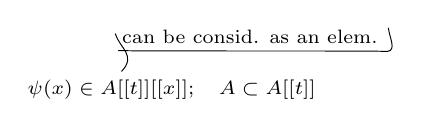
\begin{tikzpicture}[x=1mm,y=1mm,line cap=round,every node/.style={inner sep=0pt,anchor=base west,font=\scriptsize}]
\node (coefficient) at (0,0) {$\psi(x)\in A[[t]][[x]];$};
\node at ([xshift=3mm]coefficient.base east) {$A\subset A[[t]]$};
\node (insert) at (12,6.4) {can be consid. as an elem.};
\draw[line width=.35pt] ([xshift=-.4mm,yshift=-.8mm]insert.south west)
  .. controls ([xshift=4mm,yshift=-.9mm]insert.south west)
          and ([xshift=-3mm,yshift=-.8mm]insert.south east)
       .. ([xshift=1.2mm,yshift=-.9mm]insert.south east)
  to[out=8,in=-84] ([xshift=1.3mm,yshift=.2mm]insert.north east);
\draw[line width=.35pt] ([xshift=-.8mm,yshift=.4mm]insert.west)
  .. controls (11.8,5.8) and (13.9,4.9) .. (12,2.9);
\end{tikzpicture}}\endgroup}
\end{GelfandAdjacentEvidence}
\begin{GelfandAdjacentEvidence}{GELFAND-P000460}{3}


Inv. form (differential):
\SourceFigure{GELFAND-P000460}{dx-relation}{Two vertical strokes and “or” stand between the formulas.
\par\smallskip\centering\color{black}
\begingroup\color{black}\GelfandFitDiagram{\begin{tikzpicture}[x=1mm,y=1mm,every node/.style={inner sep=0pt,anchor=base west,font=\small}]
\node at (0,17) {$\psi(F(x,t))\,dF(x,t)=\psi(x)\,dx.$};
\node at (19,11.3) {\rotatebox{90}{$=$}\ \textnormal{or}};
\node at (2.6,2.5) {$\psi(F(x,t))\,\dfrac{\partial F(x,t)}{\partial x}\,dx$};
\end{tikzpicture}}\endgroup}
\end{GelfandAdjacentEvidence}
\begin{GelfandAdjacentEvidence}{GELFAND-P000460}{4}

\[
\psi(F(x,t))\,\frac{\partial F(x,t)}{\partial x}=\psi(x)
\]
($t$ is a parameter; the differential is taken only in $x$)

Set $x=0$:
\[
\begin{aligned}
\left.\psi(t)(1+\ldots)\right|_{x=0}&=\psi(0),\\
\psi(t)&=\psi(0)\,\frac{1}{\left.\dfrac{\partial F(x,t)}{\partial x}\right|_{x=0}}.
\end{aligned}
\]
These are the series that are coeffs. in the inv. differential.

Canonical form:
\[
\omega(x)=\frac{1}{\left.\dfrac{\partial F(x,y)}{\partial y}\right|_{y=0}}\,dx
\]
is an \sout{\ldots} invar. differential (simple exercise).
\Unclear{GELFAND-P000460}{invariant-mark}{A heavy vertical sign lies between the words. Its reading is uncertain.}
\end{GelfandAdjacentEvidence}
\begin{GelfandAdjacentEvidence}{GELFAND-P000460}{5}


This gives a characterization.

Consider the form. series
\[
g(x)=\int_0^x\omega(x)=x+\ldots
\]
(it is important that $A$ is a $\mathbb Q$-module! — integer denominators arise during integration)
\Unclear{GELFAND-P000460}{integration-punctuation}{An exclamation mark follows “module.”}
\end{GelfandAdjacentEvidence}
\begin{GelfandAdjacentEvidence}{GELFAND-P000460}{6}

\Unclear{GELFAND-P000460}{integration-margin}{The first word after the dash reads «появляются» (“arise”).}
\end{GelfandAdjacentEvidence}
\begin{GelfandAdjacentEvidence}{GELFAND-P000460}{7}


Integrate the relation:
\[
\begin{gathered}
\psi(F(x,t))\,dF(x,t)=\psi(x)\,dx\\
g(F(x,y))=g(x)+C;
\end{gathered}
\]
Here integration is in $x$ ($t$ — param.), therefore $C=C(y)$.

Set $x=0$. We obtain: $C=g(y)$ \sout{\ldots}
\Incomplete{GELFAND-P000460}{constant-cancel}{The entry after $C=g(y)$ is crossed out and illegible.}
\end{GelfandAdjacentEvidence}
\begin{GelfandAdjacentEvidence}{GELFAND-P000460}{8}

\[
\begin{gathered}
g(F(x,y))=g(x)+g(y)\\
F(x,y)=g^{-1}(g(x)+g(y)).\quad !!\qquad\blacksquare
\end{gathered}
\]
\uuline{Corollary}\quad Over $\mathbb Q$-mods. all form. laws are strictly isom.

Univ. law: consid. $g(x)=x+\sum g_i x^{i+1}$ — a series, its ring is $\mathbb Q[g_i]$.
\[
F(x,y)=g^{-1}(g(x)+g(y));
\]
Over $\overset{\downarrow}{\mathbb Q}[g_i]$ one obtains a univ. law.
(for all $\mathbb Q$-modules)
\Unclear{GELFAND-P000460}{base-ring-overwrite}{The letter $\mathbb Q$ below the arrow is overwritten. The earlier strokes cannot be separated.}
\end{GelfandAdjacentEvidence}
\begin{GelfandAdjacentEvidence}{GELFAND-P000460}{9}


\begin{center}
\rule[.5ex]{17mm}{.35pt}\enspace$\cdot$\enspace\rule[.5ex]{22mm}{.35pt}
\end{center}

We shall classify over arbitrary rings $A$ (commut. and with $1$)
\Unclear{GELFAND-P000460}{universal-verb}{The first word reads «Будем» (“we shall”).}
\end{GelfandAdjacentEvidence}
\begin{GelfandAdjacentEvidence}{GELFAND-P000460}{10}


\SourceFigure{GELFAND-P000460}{universal-arrow}{A curved arrow leads from the universal law to the bracket before “Universality.”
\par\smallskip\centering\color{black}
\begingroup\color{black}\GelfandFitDiagram{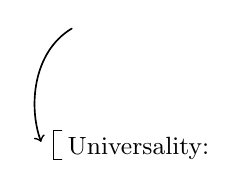
\begin{tikzpicture}[x=1mm,y=1mm,line cap=round]
\draw[->,line width=.6pt] (6,17) .. controls (1,14) and (.5,7) .. (2.1,2.6);
\draw[line width=.5pt] (4.7,4.05)--(3.7,4.05)--(3.7,.35)--(4.7,.35);
\node[anchor=base west,inner sep=0pt,font=\small] at (5.4,1) {Universality:};
\end{tikzpicture}}\endgroup}
\end{GelfandAdjacentEvidence}
\begin{GelfandAdjacentEvidence}{GELFAND-P000460}{11}

any series $F(x,y)$ over the $\mathbb Q$-mod. $A$ is obt. from such a series by replacing its coefficients by their homomorphic images under a ring homom.
$\mathbb Q[g_i]$ into $A$, sending $g_i$ to the coeffs. of the series $g(x)$,
found above\(\bigr]\)
\Unclear{GELFAND-P000460}{universal-images}{The two words for “homomorphic images” have plural endings.}
\end{GelfandAdjacentEvidence}



\Needspace{7\baselineskip}
\begin{GelfandAdjacentEvidence}{GELFAND-P000461}{1}
\SourcePage{GELFAND-P000461}{unlabelled}
\underline{Now consid. the general case}: $A$ is not necess. a $\mathbb Q$-module.

Consid. the series $F(x,y)=x+y+\sum a_{i,j}x^iy^j$

$a_{i,j}$ — alg. indep. variables.

Consid. $\mathbb Z[a_{i,j}]$,\quad $\deg a_{i,j}=i+j-1$

A form. group is obt. from it
\[
\begin{gathered}
F(F(x,y),z)=x+y+z+\sum a_{i,j,k}x^iy^jz^k,\quad
a_{i,j,k}\in\mathbb Z[a_{i,j}].\\
F(x,F(y,z))=x+y+z+\sum a'_{i,j,k}x^iy^jz^k
\qquad a'_{i,j,k}\in\mathbb Z[a_{i,j}]
\end{gathered}
\]
Consid. in $\overset{\mathbb Z[a_{i,j}]}{\text{\sout{\ldots}}}$ the ideal
$J$, gen. by the homog. elems. $\{a_{i,j,k}-a'_{i,j,k}\}$
and by the elems. $\{a_{i,j}-a_{j,i}^{\text{\sout{\ldots}}}\}$.
\Incomplete{GELFAND-P000461}{ideal-cancel}{$\mathbb Z[a_{i,j}]$ is inserted above the cancellation. The earlier entry is illegible.}
\end{GelfandAdjacentEvidence}
\begin{GelfandAdjacentEvidence}{GELFAND-P000461}{2}

\Unclear{GELFAND-P000461}{comm-coefficient}{There are crossed-out strokes above the second coefficient $a_{j,i}$.}
\end{GelfandAdjacentEvidence}
\begin{GelfandAdjacentEvidence}{GELFAND-P000461}{3}


Now replace $a_{i,j}$ in $F(x,y)$ with $a_{i,j}\bmod J$ —
\sout{\ldots} we obtain the series $F\in\Lambda[[x,y]]$.
\Incomplete{GELFAND-P000461}{cancel-before-series}{The entry before “we obtain” is crossed out and illegible.}
\end{GelfandAdjacentEvidence}
\begin{GelfandAdjacentEvidence}{GELFAND-P000461}{4}

\[
\Lambda=\mathbb Z[a_{i,j}]/J
\]
This is the univ. group. (clear).

\underline{Lazard’s thm.}, $\Lambda$ — a polynomial ring on generators, one in each dimension:
\[
\Lambda=\mathbb Z[a_i],\quad i\ge1,\quad\deg a_i=i.
\]
\Unclear{GELFAND-P000461}{one-generator-overwrite}{The penultimate letter of «одной» (“one”) is heavily overwritten.}
\end{GelfandAdjacentEvidence}
\begin{GelfandAdjacentEvidence}{GELFAND-P000461}{5}


By \underline{Lazard’s lemma}:
\SourceFigure{GELFAND-P000461}{rational-identity-divider}{Two pairs of strokes with dots lie above and below the equality.
\par\smallskip\centering\color{black}
\begingroup\color{black}\GelfandFitDiagram{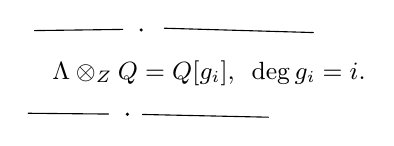
\begin{tikzpicture}[x=1mm,y=1mm,line cap=round,every node/.style={inner sep=0pt,anchor=base west,font=\small}]
\node (eq) at (3,0) {$\Lambda\otimes_{\mathbb Z}\mathbb Q=\mathbb Q[g_i],$};
\node at ([xshift=2mm]eq.base east) {$\deg g_i=i$.};
\draw (.8,6.2)--(12,6.35) (17.3,6.5)--(36.2,5.95)
      (0,-4.3)--(10.2,-4.4) (14.5,-4.45)--(30.5,-4.8);
\fill (14.35,6.28) circle (.22) (12.6,-4.42) circle (.22);
\end{tikzpicture}}\endgroup}
\end{GelfandAdjacentEvidence}
\begin{GelfandAdjacentEvidence}{GELFAND-P000461}{6}


\underline{1.}\quad How many mult. generators has $\Lambda$?

Consid. $\widetilde\Lambda=\Lambda/(\text{decomposable elements})$.
\Unclear{GELFAND-P000461}{decomposable-word}{The word in the denominator provisionally reads «разложимым» (“decomposable”).}
\end{GelfandAdjacentEvidence}
\begin{GelfandAdjacentEvidence}{GELFAND-P000461}{7}


\SourceFigure{GELFAND-P000461}{indecomposable-ideal-link}{A short vertical stroke links the first ring to the explanation.
\par\smallskip\centering\color{black}
\begingroup\color{black}\GelfandFitDiagram{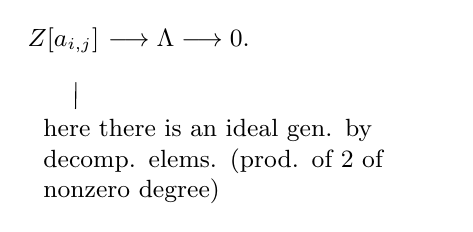
\begin{tikzpicture}[x=1mm,y=1mm,line cap=round,every node/.style={inner sep=0pt,anchor=base west,font=\small}]
\node (ring) at (0,15) {$\mathbb Z[a_{i,j}]$};
\node at ([xshift=1mm]ring.base east) {$\longrightarrow\Lambda\longrightarrow0$.};
\node[anchor=north west,text width=51mm,align=left] at (2,5.8) {here there is an ideal gen. by decomp. elems. (prod. of $2$ of nonzero degree)};
\draw (6.2,10.4)--(6.15,7.1);
\end{tikzpicture}}\endgroup}
\end{GelfandAdjacentEvidence}
\begin{GelfandAdjacentEvidence}{GELFAND-P000461}{8}


\noindent
\begin{tabular}{@{}p{.44\linewidth}@{\hspace{2mm}}||@{\hspace{2mm}}p{.49\linewidth}@{}}
\raggedright We have: $\widetilde\Lambda=\sum_{i\ge0}\widetilde\Lambda_i$;\par
multiplication is zero except when one of \sout{\ldots} is an elem. of degree $0$. &
\raggedright Decomp. elems. are elems. of the form $a\cdot b$, where $a$ and $b$ \({}^{\ast}\)\par
\({}^{\ast}\) are noninvertible. Take the ideal they generate, and $\widetilde\Lambda$ — the quotient ring.\par
Grading $\Rightarrow$ only elems. of degree $0$ are invertible.\par
Hence this ideal is the image of the ideal of decomp. elems. from $\mathbb Z[a_{i,j}]$.\tabularnewline
\end{tabular}
\SourceFigure{GELFAND-P000461}{margin-layout}{Two vertical strokes separate the marginal note at right.}
\end{GelfandAdjacentEvidence}
\begin{GelfandAdjacentEvidence}{GELFAND-P000461}{9}

\Unclear{GELFAND-P000461}{graded-sum-glyph}{The left-hand sign probably reads $\widetilde\Lambda$ with a joined tilde. Another possible reading is $\chi$.}
\end{GelfandAdjacentEvidence}
\begin{GelfandAdjacentEvidence}{GELFAND-P000461}{10}

\Incomplete{GELFAND-P000461}{pi-degree-zero}{The short entry after “of” is crossed out and illegible.}
\end{GelfandAdjacentEvidence}
\begin{GelfandAdjacentEvidence}{GELFAND-P000461}{11}

\Unclear{GELFAND-P000461}{margin-nonunits}{The marginal note reads «необратимы» (“are noninvertible”).}
\end{GelfandAdjacentEvidence}
\begin{GelfandAdjacentEvidence}{GELFAND-P000461}{12}

\Unclear{GELFAND-P000461}{margin-verb}{«Берется» (“take”) follows «необратимы».}
\end{GelfandAdjacentEvidence}
\begin{GelfandAdjacentEvidence}{GELFAND-P000461}{13}


$\widetilde\Lambda_n$ — an abelian grp. under add. with gens. — gens. of the mult. grp. $\Lambda$ in dimension $n$.
\[
F(F(x,y),z)=F(x,y)+z+\sum a_{i,j}\,\text{\sout{\ldots}}\,(x+y)^i z^j
\]
\Incomplete{GELFAND-P000461}{cancel-exponent}{The entry before $(x+y)^i$ is crossed out and illegible.}
\end{GelfandAdjacentEvidence}
\begin{GelfandAdjacentEvidence}{GELFAND-P000461}{14}


\SourceFigure{GELFAND-P000461}{product-insertion}{The bubble above the line contains “of different $a_{i,j}$.”
\par\smallskip\centering\color{black}
\begingroup\color{black}\GelfandFitDiagram{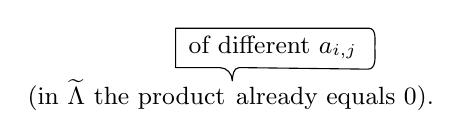
\begin{tikzpicture}[x=1mm,y=1mm,line cap=round,line join=round,every node/.style={inner sep=0pt,anchor=base west,font=\small}]
\node (prod) at (0,0) {(in $\widetilde\Lambda$ the product};
\node (rest) at ([xshift=1.2mm]prod.base east) {already equals $0$).};
\node (insert) at ([xshift=-6mm,yshift=6.5mm]rest.base west) {of different $a_{i,j}$};
\draw ([xshift=-1.6mm,yshift=.9mm]insert.north west)
   -- ([xshift=1.4mm,yshift=.9mm]insert.north east)
   to[out=0,in=90] ([xshift=2.2mm]insert.east)
   to[out=-90,in=0] ([xshift=1.3mm,yshift=-1.2mm]insert.south east)
   -- ([xshift=6.5mm,yshift=-1mm]insert.south west)
   to[out=180,in=86] ([xshift=-.4mm,yshift=.55mm]rest.north west)
   to[out=90,in=0] ([xshift=4mm,yshift=-1mm]insert.south west)
   -- ([xshift=-1.6mm,yshift=-1mm]insert.south west)
   -- cycle;
\end{tikzpicture}}\endgroup}
\end{GelfandAdjacentEvidence}

\[
F(x,F(y,z))=x+F(y,z)+\sum a_{i,j}x^i(y+z)^j
\]
$\widetilde\Lambda$ is obt. from the free ab. group gen. by $a_{i,j}$, by quotienting by the rels. \ldots

Let $h(x,y)=\sum h_{i,j}x^iy^j=F(x,y)-x-y$.
\[
h(x,0)=0,\quad h(0,y)=0.
\]


\Needspace{7\baselineskip}
\begin{GelfandAdjacentEvidence}{GELFAND-P000462}{1}
\SourcePage{GELFAND-P000462}{unlabelled}
Lazard’s rel.:
\[
\uwave{\mbox{$h(x,y)+h(x+y,z)=h(y,z)+h(x,y+z).$}}\qquad(*)
\]
It suffices to take homog. polynomials $h$.

In Lazard: methods of number theory.

\uwave{Problem:}\quad find all solutions of $(*)$ [homog. polys.] over some ring $K$.

All solutions — \uwave{a group \mbox{$L$}},\quad Everything over the ring $K$
\[
L\longrightarrow\operatorname{Ext}_{K[x]}^{2,n}(K,K)\longrightarrow0.
\]
Introduce on $K[x]$ a Hopf struct.: a mult. homomorphism
\[
\begin{gathered}
\Delta:K[x]\longrightarrow K[x]\otimes_K K[x]\qquad\text{(comultiplication).}\\
x\longrightarrow x\otimes1+1\otimes x
\end{gathered}
\]
A Hopf alg. has cohomology. The alg. is graded $\Rightarrow$ the cohom. is bigraded.
Hence $2$ indices for $\operatorname{Ext}$.

Next:
\[
\begin{aligned}
 &\quad\text{on the left and on the right}\quad (x+y+z)^n-x^n-y^n-z^n\\[-.2ex]
 &\qquad\downarrow\\[-.2ex]
 0&\longrightarrow
 \{c((x+y)^n-x^n-y^n),\,a\in K\}
 \longrightarrow L\longrightarrow
 \operatorname{Ext}_{K[x]}^{2,n}(K,K)\longrightarrow0.
\end{aligned}
\]
\SourceFigure{GELFAND-P000462}{sequence-arrow}{The arrow from the addition points down toward the first term of the sequence.}
\end{GelfandAdjacentEvidence}
\begin{GelfandAdjacentEvidence}{GELFAND-P000462}{2}

\Unclear{GELFAND-P000462}{family-coefficient}{The sign before the parentheses provisionally reads $c$. The separate entry reads $a\in K$. Both signs are overwritten.}
\end{GelfandAdjacentEvidence}
\begin{GelfandAdjacentEvidence}{GELFAND-P000462}{3}


\begin{center}
\rule[.5ex]{17mm}{.35pt}\enspace$\cdot$\enspace\rule[.5ex]{22mm}{.35pt}
\end{center}

\uuline{\mbox{$n=2$}}.\quad
$\overset{\text{\sout{\ldots}}}{\text{Polyn.}}$ of degree $2$
\uuline{\mbox{$cxy$}}.
\Unclear{GELFAND-P000462}{cancel-n2}{The sign above “Polyn.” is crossed out and illegible.}
\end{GelfandAdjacentEvidence}
\begin{GelfandAdjacentEvidence}{GELFAND-P000462}{4}


\uuline{\mbox{$n=3$}}\quad $h(x,y)=C_1x^2y+C_2xy^2$
\[
\widetilde\Lambda=\mathbb Z+\mathbb Z_3.
\]
\Unclear{GELFAND-P000462}{cubic-quotient}{The line reads $\widetilde\Lambda=\mathbb Z+\mathbb Z_3$.}
\end{GelfandAdjacentEvidence}
\begin{GelfandAdjacentEvidence}{GELFAND-P000462}{5}


$1$ sol. by Lazard’s lemma: $c((x+y)^n-x^n-y^n)$

$h(x,y)=x^2y+xy^2$\qquad for all rings

$h(x,y)=x^2y$\qquad for rings that are $\mathbb Z_3$-modules
\Unclear{GELFAND-P000462}{cubic-module-claim}{The subscript on $\mathbb Z$ in this line is $3$.}
\end{GelfandAdjacentEvidence}
\begin{GelfandAdjacentEvidence}{GELFAND-P000462}{6}


\noindent\hspace*{1.7em}$x^2y$

\begin{center}
\rule[.5ex]{26mm}{.35pt}\enspace$\cdot$\enspace\rule[.5ex]{27mm}{.35pt}
\end{center}
Consid. comodules over a Hopf alg. $A$ — this is an ab. grp. $N$, for which there is a map $N\longrightarrow A\otimes N$ with nat. conds.
\begin{center}
\rule[.5ex]{25mm}{.35pt}\enspace$\cdot$\enspace\rule[.5ex]{29mm}{.35pt}
\end{center}

Choose the resolution correctly: there will be all cycles without boundaries (min. resolution). \sout{by}
\Unclear{GELFAND-P000462}{cancel-after-resolution}{The crossed-out word after the parenthesis may read «по» (“by”).}
\end{GelfandAdjacentEvidence}
\begin{GelfandAdjacentEvidence}{GELFAND-P000462}{7}

\begin{center}
\rule[.5ex]{26mm}{.35pt}\enspace$\cdot$\enspace\rule[.5ex]{29mm}{.35pt}
\end{center}

\sout{Н\ldots}
\Unclear{GELFAND-P000462}{cancel-heading-fragment}{The start of the crossed-out heading shows the Cyrillic «Н».}
\end{GelfandAdjacentEvidence}
\begin{GelfandAdjacentEvidence}{GELFAND-P000462}{8}

\Incomplete{GELFAND-P000462}{cancel-heading-remainder}{The rest of the crossed-out heading is illegible.}
\end{GelfandAdjacentEvidence}
\begin{GelfandAdjacentEvidence}{GELFAND-P000462}{9}


\uuline{Calculation of the group \mbox{$\operatorname{Ext}^2$}.}

$1^\circ$. $K$ — \sout{\ldots} a comodule over the Hopf alg. $K[x]$.
\Unclear{GELFAND-P000462}{cancel-comodule}{A heavy rectangular mark is crossed out between the dash after $K$ and “comodule.”}
\end{GelfandAdjacentEvidence}
\begin{GelfandAdjacentEvidence}{GELFAND-P000462}{10}


\hfill\sout{\ldots}\quad $x\longrightarrow x\otimes1+1\otimes x$\par
\Unclear{GELFAND-P000462}{coproduct-mark}{A heavily crossed-out sign appears before $x$ in the addition.}
\end{GelfandAdjacentEvidence}
\begin{GelfandAdjacentEvidence}{GELFAND-P000462}{11}

\[
K\longrightarrow K\otimes K[x]\quad
\text{\sout{\mbox{$\gets$}\ldots}}
\]
\Unclear{GELFAND-P000462}{cancel-after-tensor-fragment}{The beginning of the crossed-out addition resembles $\gets$.}
\end{GelfandAdjacentEvidence}
\begin{GelfandAdjacentEvidence}{GELFAND-P000462}{12}

\Incomplete{GELFAND-P000462}{cancel-after-tensor-remainder}{The remaining strokes after $K[x]$ are illegible.}
\end{GelfandAdjacentEvidence}


$1\longrightarrow1\otimes1$\qquad and then by linearity.


\Needspace{7\baselineskip}
\begin{GelfandAdjacentEvidence}{GELFAND-P000463}{1}
\SourcePage{GELFAND-P000463}{unlabelled}
Consid.
\[
K_*[x]=\operatorname{Hom}_K(K[x],K).
\]
(“diff. operators”).
\[
(x_*^n,x^m)=\delta_{n,m}
\]
Multiplication:
\[
\underline{x_*^n\cdot x_*^m=C_{n+m}^n x_*^{n+m}}
\qquad\text{— \underline{table}.}
\]
Here $K$ plays no role.

It suffices to take $K=\mathbb Z_p$ or $\mathbb Q$.
\[
K_*[x]=\prod_{q=1}^\infty B_q,\qquad
B_q=\mathbb Z_p[y_{p^i}]/(y_{p^i}^{\,p})
\]
\Unclear{GELFAND-P000463}{product-factorization}{The left side reads $K_*[x]$. The product has lower limit $q=1$ and upper limit $\infty$.}
\end{GelfandAdjacentEvidence}
\begin{GelfandAdjacentEvidence}{GELFAND-P000463}{2}


$y_1,\ldots,y_i,\ldots,y_{p^i}$ — generators.
\Unclear{GELFAND-P000463}{generator-powers}{In three places the $i$ next to $p$ is raised. This is set as $y_{p^i}$. In the denominator the separate outer exponent $p$ on $y$ is visible.}
\end{GelfandAdjacentEvidence}



\Needspace{7\baselineskip}
\begin{GelfandAdjacentEvidence}{GELFAND-P000464}{1}
\SourcePage{GELFAND-P000464}{unlabelled}
\underline{30/\mbox{$\overline{\underline{\mathrm X}}$}-72.}
\quad\underline{Gelfand sem..}

\underline{I. Bernstein}

\uuline{И.М.Г.}

\SourceFigure{GELFAND-P000464}{general-graph}{The two arrows at left point to the same vertex. From the middle vertex arrows lead left, right and down to the right. The bent line at right has arrowheads. The small strokes at vertices have no established reading as letters.
\par\smallskip\centering\color{black}
\begingroup\color{black}\GelfandFitDiagram{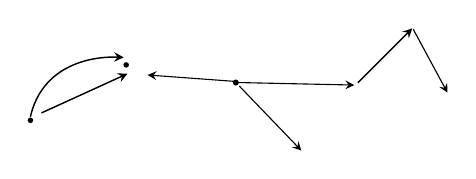
\begin{tikzpicture}[x=.16mm,y=-.16mm,line cap=round,line join=round,>=stealth]
\fill (20,91) circle (1pt) (96,47) circle (1pt) (183,61) circle (1.1pt);
\draw[->,line width=.52pt] (20,88)
 .. controls (29,49) and (65,40) .. (94,41);
\draw[->,line width=.52pt] (29,85)--(97,54);
\draw[->] (181,60)--(113,55);
\draw[->] (185,61)--(277,63);
\draw[->] (186,64)--(235,115);
\draw[->,line width=.5pt] (280,61)--(323,18);
\draw[->] (324,19)--(351,69);
\end{tikzpicture}}\endgroup}
\end{GelfandAdjacentEvidence}
\begin{GelfandAdjacentEvidence}{GELFAND-P000464}{2}


There is a directed graph. This is a category.

\sout{Р}\quad Consid. some diagrams, with at the points — vect. spaces,
on the arrows maps (functoriality is not required).
\Unclear{GELFAND-P000464}{cancel-before-consider}{A loop survives at the start of the crossed-out sign. Possibly Cyrillic «Р».}
\end{GelfandAdjacentEvidence}
\begin{GelfandAdjacentEvidence}{GELFAND-P000464}{3}

\Unclear{GELFAND-P000464}{diagram-adjective}{The words before “diagrams” provisionally read «какие л.» (“some”).}
\end{GelfandAdjacentEvidence}
\begin{GelfandAdjacentEvidence}{GELFAND-P000464}{4}


Prob. — to classify.

\SourceFigure{GELFAND-P000464}{one-arrow}{A slightly curved rightward arrow joins the two points.
\par\smallskip\centering\color{black}
\begingroup\color{black}\GelfandFitDiagram{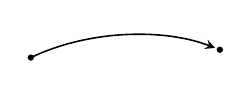
\begin{tikzpicture}[x=1mm,y=1mm,line cap=round,>=stealth]
\fill (0,0) circle (1.15pt) (24,1) circle (1.15pt);
\draw[->,line width=.57pt,shorten >=.65mm] (0,0)
  .. controls (7.5,3.6) and (17,3.7) .. (24,1);
\end{tikzpicture}}\endgroup}
\end{GelfandAdjacentEvidence}
\begin{GelfandAdjacentEvidence}{GELFAND-P000464}{5}


Prob. of classif. of maps.\quad The only invs. are $\dim\operatorname{Ker}$ and $\dim\operatorname{Coker}$.
Reduces to an embedding.

\SourceFigure{GELFAND-P000464}{one-loop}{One loop. Its arrowhead on the left side points upward.
\par\smallskip\centering\color{black}
\begingroup\color{black}\GelfandFitDiagram{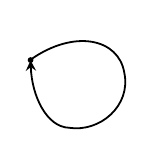
\begin{tikzpicture}[x=1mm,y=1mm,line cap=round,line join=round,>=stealth]
\fill (0,1.4) circle (1.05pt);
\draw[->,line width=.65pt] (0,1.45)
  .. controls (5.6,5.4) and (11.2,4.1) .. (11.9,-.2)
  .. controls (12.8,-4.4) and (8.8,-7.8) .. (4.9,-7.2)
  .. controls (2,-7.1) and (.15,-3.1) .. (0,1.35);
\end{tikzpicture}}\endgroup}
\end{GelfandAdjacentEvidence}
\begin{GelfandAdjacentEvidence}{GELFAND-P000464}{6}


one transformation.

\SourceFigure{GELFAND-P000464}{two-loop}{Two loops share the left vertex. The top of the outer loop is faint. Overlapping arrowhead strokes are visible near the vertex.
\par\smallskip\centering\color{black}
\begingroup\color{black}\GelfandFitDiagram{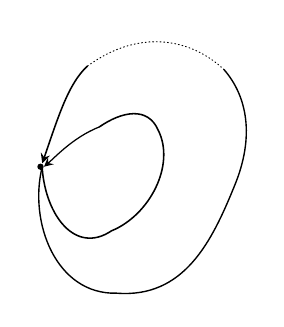
\begin{tikzpicture}[x=.22mm,y=-.22mm,line cap=round,line join=round,>=stealth]
\fill (20,83) circle (1.15pt);
\draw[line width=.5pt] (21,83)
 .. controls (13,115) and (29,157) .. (64,156)
 .. controls (103,159) and (119,126) .. (132,94)
 .. controls (144,65) and (139,42) .. (126,27);
\draw[densely dotted,line width=.34pt] (126,27)
 .. controls (107,9) and (77,3) .. (47,25);
\draw[->,line width=.56pt] (47,25)
 .. controls (36,35) and (30,55) .. (21,81);
\draw[line width=.56pt] (21,84)
 .. controls (23,111) and (40,134) .. (61,120)
 .. controls (83,111) and (98,82) .. (88,62)
 .. controls (82,48) and (67,51) .. (54,60);
\draw[->,line width=.45pt] (54,60) .. controls (39,66) and (29,77) .. (22,83);
\end{tikzpicture}}\endgroup}
\end{GelfandAdjacentEvidence}
\begin{GelfandAdjacentEvidence}{GELFAND-P000464}{7}


— the prob. is unsolvable (a pair of arbitrary lin. operators). \sout{\ldots}
\Unclear{GELFAND-P000464}{cancel-before-ona}{The short entry before “it” is crossed out and illegible.}
\end{GelfandAdjacentEvidence}
\begin{GelfandAdjacentEvidence}{GELFAND-P000464}{8}


It reduces to the prob. of commuting ones (Gelf. and Ponomarev).
\Unclear{GELFAND-P000464}{wild-name}{The first letter is overwritten. The abbreviation reads «Гельф.» (Gelf.).}
\end{GelfandAdjacentEvidence}
\begin{GelfandAdjacentEvidence}{GELFAND-P000464}{9}


\sout{Reduc.\ldots}
\Unclear{GELFAND-P000464}{large-cancel-fragment}{The crossed-out line may begin «Свод.» (“reduc.”).}
\end{GelfandAdjacentEvidence}
\begin{GelfandAdjacentEvidence}{GELFAND-P000464}{10}

\Incomplete{GELFAND-P000464}{large-cancel-remainder}{The remainder of the crossed-out line is illegible.}
\end{GelfandAdjacentEvidence}
\begin{GelfandAdjacentEvidence}{GELFAND-P000464}{11}


\[
\left.
\begin{gathered}
\text{Space and subspace.}\\
\text{Space and 2 subspaces}
\end{gathered}
\right\}\quad\text{triv.}
\]
Can be done:\quad Space and \uwave{\mbox{$3$} lin. subspaces}.
\Unclear{GELFAND-P000464}{three-space-word}{The start of the line provisionally reads «Делается» (“can be done”).}
\end{GelfandAdjacentEvidence}
\begin{GelfandAdjacentEvidence}{GELFAND-P000464}{12}


There are $9$, invariants, not $8$!

\SourceFigure{GELFAND-P000464}{three-inward}{Three arrows point toward the upper vertex. Their arrowheads partly merge.
\par\smallskip\centering\color{black}
\begingroup\color{black}\GelfandFitDiagram{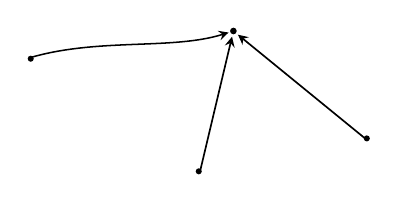
\begin{tikzpicture}[x=.22mm,y=-.22mm,line cap=round,>=stealth]
\fill (22,45) circle (1.1pt) (139,29) circle (1.2pt)
      (119,110) circle (1.1pt) (216,91) circle (1.1pt);
\draw[->,line width=.55pt,shorten >=.65mm] (23,44)
 .. controls (62,33) and (104,40) .. (139,29);
\draw[->,line width=.6pt,shorten >=.75mm] (120,109)--(139,29);
\draw[->,line width=.6pt,shorten >=.75mm] (215,91)--(139,29);
\end{tikzpicture}}\endgroup}
\end{GelfandAdjacentEvidence}
\begin{GelfandAdjacentEvidence}{GELFAND-P000464}{13}

(problem).

\SourceFigure{GELFAND-P000464}{four-inward}{Four edges meet at the heavily inked central vertex. Overlapping strokes obscure the direction of two edges.
\par\smallskip\centering\color{black}
\begingroup\color{black}\GelfandFitDiagram{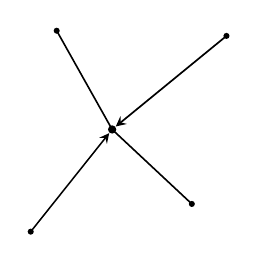
\begin{tikzpicture}[x=.22mm,y=-.22mm,line cap=round,>=stealth]
\fill (31,30) circle (1.1pt) (129,33) circle (1.1pt)
      (16,146) circle (1.1pt) (109,130) circle (1.1pt)
      (63,87) circle (1.5pt);
\draw[line width=.58pt] (31,30)--(63,87)--(109,130);
\draw[->,line width=.61pt,shorten >=.6mm] (129,33)--(63,87);
\draw[->,line width=.55pt,shorten >=.6mm] (16,146)--(63,87);
\end{tikzpicture}}\endgroup}
\end{GelfandAdjacentEvidence}
\begin{GelfandAdjacentEvidence}{GELFAND-P000464}{14}


Space and $4$ subspaces classified (Gelf. and Ponom.) —
\sout{\ldots} already an inf. number of indecomp.
\Incomplete{GELFAND-P000464}{cancel-after-names}{The word after the dash is crossed out and illegible.}
\end{GelfandAdjacentEvidence}


\underline{Gabriel}: in which graphs are there finitely many indecomp. systems?

Answer: draw a Dynkin diagram! — these and only these are such graphs.

Exceptions: diagrams with double (generally multiple) arrows.


\Needspace{7\baselineskip}
\begin{GelfandAdjacentEvidence}{GELFAND-P000465}{1}
\SourcePage{GELFAND-P000465}{unlabelled}
\underline{Theorem}\quad
(\begin{tabular}[t]{@{}c@{}}Roytov\\[-.45ex]\scriptsize from Kyiv\end{tabular}
or Nazarovy).
\Unclear{GELFAND-P000465}{theorem-names}{The names provisionally read «Ройтов» and «Назаровы». The addition below reads “from Kyiv.”}
\end{GelfandAdjacentEvidence}
\begin{GelfandAdjacentEvidence}{GELFAND-P000465}{2}


A class of diagrams is descr. with a classific. as in Gelf. and Ponomarev.

\uwave{Connection \sout{\ldots}\ with singularities!}\quad — see Artin, Tyurina, Brieskorn.
\Incomplete{GELFAND-P000465}{cancel-specialities}{The word between “Connection” and “with singularities” is crossed out and illegible.}
\end{GelfandAdjacentEvidence}
\begin{GelfandAdjacentEvidence}{GELFAND-P000465}{3}


\begin{center}
\rule[.5ex]{18mm}{.35pt}\enspace$\cdot$\enspace\rule[.5ex]{25mm}{.35pt}
\end{center}

\uuline{И.Б.}\quad \uwave{Category of} vect. spaces over points and maps over arrows.

(The graph is fixed). \quad \uwave{Def. direct sum}. This is $\operatorname{Cat}(\Gamma)$
($\Gamma$ — graph)

Morphisms — maps over each point with commut. diagrs.

$\bullet$\qquad category of linear spaces.

Important: no need to ident. isomorphic ones.
\Unclear{GELFAND-P000465}{important-line}{The abbreviation before “isomorphic” provisionally reads «отожд.» (“ident.”).}
\end{GelfandAdjacentEvidence}
\begin{GelfandAdjacentEvidence}{GELFAND-P000465}{4}


It is easy to see that $\forall$ object $=\sum$ indecomp. ones. (uniquely up to isom.).

$1)$\quad \uwave{Classif. \mbox{$\Gamma$}, with finitely many indecomp. objects.}

\underline{Restrict to connected ones}:

\SourceFigure{GELFAND-P000465}{dynkin-a-mark}{A small angular stroke rises above the third vertex from the left.
\par\smallskip\centering\color{black}
\begingroup\color{black}\GelfandFitDiagram{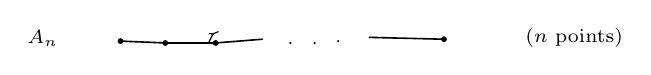
\begin{tikzpicture}[x=.079mm,y=-.079mm,line cap=round,every node/.style={font=\scriptsize,inner sep=0pt}]
\node at (52,58) {$A_n$};
\draw[line width=.58pt] (177,62)--(249,65)--(330,65)--(405,59);
\draw[line width=.58pt] (577,56)--(697,59);
\foreach \x/\y in {177/62,249/65,330/65,697/59}{\fill (\x,\y) circle (1.06pt);}
\foreach \x/\y in {450/65,489/65,527/62}{\fill (\x,\y) circle (.44pt);}
\draw[line width=.44pt] (319,64)--(326,50)--(320,50) (324,51)--(334,47);
\node[anchor=west] at (827,56) {($n$ points)};
\end{tikzpicture}}\endgroup}
\end{GelfandAdjacentEvidence}
\begin{GelfandAdjacentEvidence}{GELFAND-P000465}{5}


\SourceFigure{GELFAND-P000465}{dynkin-d}{There is a small leftward arrowhead on the segment between the third and fourth vertices.
\par\smallskip\centering\color{black}
\begingroup\color{black}\GelfandFitDiagram{\begin{tikzpicture}[x=.074mm,y=-.074mm,line cap=round,every node/.style={font=\scriptsize,inner sep=0pt}]
\node at (50,63) {$D_n$};
\draw[line width=.57pt] (164,64)--(253,63)--(328,66);
\draw[line width=.57pt] (346,65)--(402,63)--(445,64);
\draw[line width=.43pt] (348,61)--(341,65)--(348,69);
\draw[line width=.57pt] (603,67)--(696,65)--(774,21) (696,65)--(764,118);
\foreach \x/\y in {164/64,253/63,328/66,402/63,603/67,696/65,774/21,764/118}
  {\fill (\x,\y) circle (1.04pt);}
\foreach \x/\y in {459/72,496/67,525/67}{\fill (\x,\y) circle (.47pt);}
\node[anchor=west] at (1010,66) {$n\ge4$};
\end{tikzpicture}}\endgroup}
\end{GelfandAdjacentEvidence}
\begin{GelfandAdjacentEvidence}{GELFAND-P000465}{6}


\SourceFigure{GELFAND-P000465}{dynkin-e}{There are six vertices on the horizontal chain. A branch descends from the third vertex from the left.
\par\smallskip\centering\color{black}
\begingroup\color{black}\GelfandFitDiagram{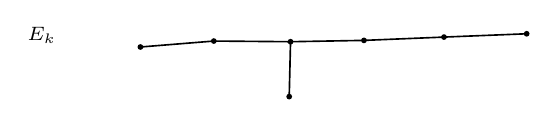
\begin{tikzpicture}[x=.084mm,y=-.084mm,line cap=round,every node/.style={font=\scriptsize,inner sep=0pt}]
\node at (45,53) {$E_k$};
\draw[line width=.59pt] (194,70)--(305,61)--(421,62)--(532,60)--(653,55)--(778,50);
\draw[line width=.6pt] (421,62)--(419,145);
\foreach \x/\y in {194/70,305/61,421/62,532/60,653/55,778/50,419/145}
  {\fill (\x,\y) circle (1.04pt);}
\end{tikzpicture}}\endgroup}
\end{GelfandAdjacentEvidence}
\begin{GelfandAdjacentEvidence}{GELFAND-P000465}{7}

$k=6,7,8$\qquad (necessarily $2$ segments on the left).

Place the arrows arbitrarily!!

$D_4$ — space and $3$ subspaces.

Idea: no cycles (one obt. eigenvalues), no
\Unclear{GELFAND-P000465}{idea-word}{The abbreviation in parentheses may read «получ.» (“obt.”).}
\end{GelfandAdjacentEvidence}
\begin{GelfandAdjacentEvidence}{GELFAND-P000465}{8}


\SourceFigure{GELFAND-P000465}{forbidden-four}{Four segments meet at the black dot. No separate vertices are visible at the ends.
\par\smallskip\centering\color{black}
\begingroup\color{black}\GelfandFitDiagram{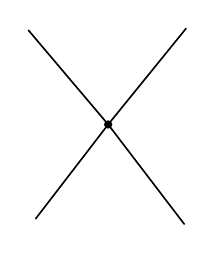
\begin{tikzpicture}[x=.23mm,y=-.23mm,line cap=round]
\draw[line width=.59pt] (16,14)--(60,66)--(102,121)
      (103,13)--(60,66)--(20,118);
\fill (60,66) circle (1.5pt);
\end{tikzpicture}}\endgroup}
\end{GelfandAdjacentEvidence}
\begin{GelfandAdjacentEvidence}{GELFAND-P000465}{9}

— there will be an inf. number.

\SourceFigure{GELFAND-P000465}{forbidden-forks}{The chain has a fork at each end. Five vertices are marked on the chain itself.
\par\smallskip\centering\color{black}
\begingroup\color{black}\GelfandFitDiagram{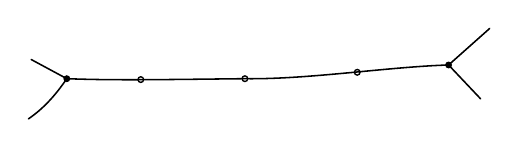
\begin{tikzpicture}[x=.116mm,y=-.116mm,line cap=round]
\draw[line width=.56pt] (18,51)--(57,72)
 .. controls (109,74) and (161,73) .. (252,72)
 .. controls (321,73) and (409,59) .. (475,57)
 -- (520,17);
\draw[line width=.56pt] (57,72)..controls(44,91)and(31,105)..(15,116)
   (475,57)--(510,94);
\fill (57,72) circle (1.25pt) (475,57) circle (1.25pt);
\foreach \x/\y in {138/73,252/72,375/65}{\draw[line width=.5pt] (\x,\y) circle (1.02pt);}
\end{tikzpicture}}\endgroup}
\end{GelfandAdjacentEvidence}
\begin{GelfandAdjacentEvidence}{GELFAND-P000465}{10}

— also imposs., since ident.
\Unclear{GELFAND-P000465}{fork-explanation}{The last abbreviation provisionally reads «отожд.» (“ident.”).}
\end{GelfandAdjacentEvidence}
\begin{GelfandAdjacentEvidence}{GELFAND-P000465}{11}


$2)$\quad \uwave{The no. of indecomp. objs. does not depend on the dir. of the arrows.}

\uwave{It is characterized by the set of dimensions}!!

one should consid. the root syst.

$\gamma$ — pos. root,\qquad $\alpha_i$ — simp. roots.

To each root — an indecomp. object
\[
\gamma=\sum n_i\alpha_i,\qquad n_i\text{ — dimensions!!}
\]
\Unclear{GELFAND-P000465}{root-symbol}{Both signs have a lower loop and two upper strokes. They are provisionally set as $\gamma$.}
\end{GelfandAdjacentEvidence}
\begin{GelfandAdjacentEvidence}{GELFAND-P000465}{12}


No. $=$ no. of simple roots.
\Unclear{GELFAND-P000465}{root-count}{The line reads «простых корней» (“simple roots”).}
\end{GelfandAdjacentEvidence}
\begin{GelfandAdjacentEvidence}{GELFAND-P000465}{13}


\SourceFigure{GELFAND-P000465}{a3-example}{Six rows of dimensions stand below the chain with two rightward arrows.
\par\smallskip\centering\color{black}
\begingroup\color{black}\GelfandFitDiagram{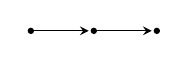
\begin{tikzpicture}[x=1mm,y=1mm,>=stealth,line cap=round]
\fill (0,0) circle (1.15pt) (8,0) circle (1.15pt) (16,0) circle (1.15pt);
\draw[->,shorten >=.65mm] (0,0)--(8,0);
\draw[->,shorten >=.65mm] (8,0)--(16,0);
\end{tikzpicture}}\endgroup\par\smallskip
$\begin{array}{ccc}
1&0&0\\
0&1&0\\
0&0&1\\
1&1&0\\
0&1&1\\
1&1&1
\end{array}$}
\end{GelfandAdjacentEvidence}
\begin{GelfandAdjacentEvidence}{GELFAND-P000465}{14}

\Unclear{GELFAND-P000465}{array-overwrite}{The middle 1 in row two is overwritten. A remnant of a loop survives to its right.}
\end{GelfandAdjacentEvidence}



\Needspace{7\baselineskip}
\begin{GelfandAdjacentEvidence}{GELFAND-P000466}{1}
\SourcePage{GELFAND-P000466}{unlabelled}
$3)$\quad \uwave{Consid. the \mbox{$\Gamma$}, for which \mbox{$\operatorname{Cat}(\Gamma)$} is solvable.}

\SourceFigure{GELFAND-P000466}{loop-category}{The two loops share a vertex. Inside the upper loop there is a short slanted stroke separate from its arrowhead.
\par\smallskip\centering\color{black}
\begingroup\color{black}\GelfandFitDiagram{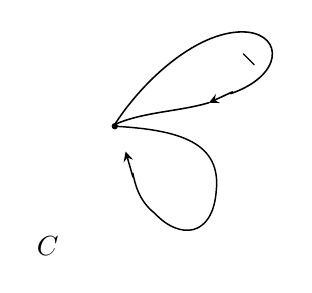
\begin{tikzpicture}[x=.23mm,y=-.23mm,line cap=round,line join=round,>=stealth]
\fill (72,63) circle (1.15pt);
\draw[line width=.56pt] (72,62)
  .. controls (88,37) and (119,9) .. (145,11)
  .. controls (165,13) and (165,35) .. (136,45);
\draw[->,line width=.57pt] (137,44)--(124,50);
\draw[line width=.56pt] (124,50)..controls(107,55)and(88,55)..(72,62);
\draw[line width=.53pt] (72,63)
  .. controls (108,65) and (131,72) .. (128,99)
  .. controls (126,124) and (108,126) .. (94,111)
  .. controls (85,104) and (83,94) .. (82,89);
\draw[->,line width=.55pt] (82,91)--(78,77);
\draw[line width=.42pt] (143,23)--(149,29);
\node at (35,129) {$C$};
\end{tikzpicture}}\endgroup}
\end{GelfandAdjacentEvidence}
\begin{GelfandAdjacentEvidence}{GELFAND-P000466}{2}


Unsolvable categ. — if there is an embedding $C\longrightarrow\operatorname{Cat}(\Gamma)$,
taking nonisom. objects to nonisom. ones.

They are classif. and correspond to extended Dynkin diagrams!

\SourceFigure{GELFAND-P000466}{three-arrow}{Three arrows leave one vertex, upward, rightward and down to the left.
\par\smallskip\centering\color{black}
\begingroup\color{black}\GelfandFitDiagram{\begin{tikzpicture}[x=.22mm,y=-.22mm,line cap=round,>=stealth]
\fill (83,101) circle (1.2pt);
\draw[->,line width=.62pt] (83,101)--(83,21);
\draw[->,line width=.59pt] (83,101)..controls(116,94)and(158,97)..(204,93);
\draw[->,line width=.6pt] (83,101)--(24,171);
\end{tikzpicture}}\endgroup}
\end{GelfandAdjacentEvidence}
\begin{GelfandAdjacentEvidence}{GELFAND-P000466}{3}


\SourceFigure{GELFAND-P000466}{affine-a}{Seven points lie on a straight chain. An arc joins the endpoints.
\par\smallskip\centering\color{black}
\begingroup\color{black}\GelfandFitDiagram{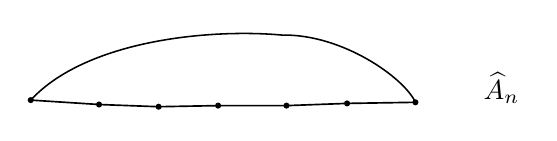
\begin{tikzpicture}[x=.14mm,y=-.14mm,line cap=round]
\draw[line width=.6pt] (22,82)--(84,86)--(138,88)--(192,87)--(254,87)--(309,85)--(371,84);
\draw[line width=.56pt] (22,82)..controls(72,28)and(183,17)..(250,23)
  ..controls(305,22)and(361,62)..(371,84);
\foreach \x/\y in {22/82,84/86,138/88,192/87,254/87,309/85,371/84}
 {\fill (\x,\y) circle (1.1pt);}
\node at (449,71) {$\widehat A_n$};
\end{tikzpicture}}\endgroup}
\end{GelfandAdjacentEvidence}
\begin{GelfandAdjacentEvidence}{GELFAND-P000466}{4}


\SourceFigure{GELFAND-P000466}{affine-d}{Seven points lie along the chain, with two branches at each end.
\par\smallskip\centering\color{black}
\begingroup\color{black}\GelfandFitDiagram{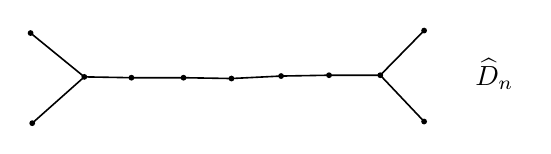
\begin{tikzpicture}[x=.105mm,y=-.105mm,line cap=round]
\draw[line width=.58pt] (24,23)--(89,76)--(146,77)--(209,77)--(267,78)--(327,75)--(385,74)--(447,74)--(500,20);
\draw[line width=.58pt] (26,132)--(89,76) (447,74)--(500,130);
\foreach \x/\y in {24/23,26/132,89/76,146/77,209/77,267/78,327/75,385/74,447/74,500/20,500/130}
 {\fill (\x,\y) circle (1.05pt);}
\node at (585,73) {$\widehat D_n$};
\end{tikzpicture}}\endgroup}
\end{GelfandAdjacentEvidence}
\begin{GelfandAdjacentEvidence}{GELFAND-P000466}{5}


\SourceFigure{GELFAND-P000466}{affine-e}{Seven points lie along the horizontal chain. Two segments with points descend from the third point from the left.
\par\smallskip\centering\color{black}
\begingroup\color{black}\GelfandFitDiagram{\begin{tikzpicture}[x=.118mm,y=-.118mm,line cap=round]
\draw[line width=.57pt] (35,77)--(83,76)--(147,73)--(204,72)--(262,72)--(325,71)--(376,73);
\draw[line width=.57pt] (147,73)--(150,134)--(151,185);
\foreach \x/\y in {35/77,83/76,147/73,204/72,262/72,325/71,376/73,150/134,151/185}
 {\fill (\x,\y) circle (1.08pt);}
\node at (500,72) {$\widehat E_n$};
\end{tikzpicture}}\endgroup}
\end{GelfandAdjacentEvidence}
\begin{GelfandAdjacentEvidence}{GELFAND-P000466}{6}


(appear in the theory of \(\overset{\text{\sout{grp.}}}{\vphantom{x}}\) groups generated by reflections.)
\Unclear{GELFAND-P000466}{cancel-in-group-comment}{The crossed-out insertion above the line may read «гр» (“grp.”).}
\end{GelfandAdjacentEvidence}
\begin{GelfandAdjacentEvidence}{GELFAND-P000466}{7}


These are all the graphs for which the prob. is solvable.

\uuline{V. Buchstaber.}

\uuline{Lazur’s thm.}
\Unclear{GELFAND-P000466}{theorem-name}{The name provisionally reads «Лазура» here. The middle vowel may be «а».}
\end{GelfandAdjacentEvidence}
\begin{GelfandAdjacentEvidence}{GELFAND-P000466}{8}

\[
\Lambda=\mathbb Z[a_1,\ldots,a_n,\ldots],\qquad\deg a_n=n\ge1.
\]
\underline{Proof.}
\[
\Lambda\longrightarrow\bar\Lambda=\Lambda/(\text{decomp.})
\]
\Unclear{GELFAND-P000466}{decomposables-quotient}{A horizontal stroke stands above the second $\Lambda$. The denominator reads «разл.» (“decomp.”).}
\end{GelfandAdjacentEvidence}
\begin{GelfandAdjacentEvidence}{GELFAND-P000466}{9}


$\bar\Lambda$ — \uwave{univ. ring for}
\(\underset{\downarrow}{\boxed{\text{\scriptsize such}}}\)
\uwave{polynomials} $h(x,y)$,
\SourceFigure{GELFAND-P000466}{such-insertion}{“Such” is inserted in a bubble before “polynomials.”}
\end{GelfandAdjacentEvidence}
\begin{GelfandAdjacentEvidence}{GELFAND-P000466}{10}


\(\underset{\downarrow}{\boxed{\text{\scriptsize that}}}\)\quad
$h(x,y)=h(y,x)$,\quad $h(x,0)=0$,
\[
h(y,z)+h(x,y+z)=h(x,z)+h(y,x+z).
\]
\SourceFigure{GELFAND-P000466}{that-insertion}{“That” is inserted in a separate bubble before the conditions.}
\end{GelfandAdjacentEvidence}
\begin{GelfandAdjacentEvidence}{GELFAND-P000466}{11}


This is cohomology:\quad $\underset{\text{(cycles)}}{dh}=0$
\qquad (in the bar construction for polynomials)
\Unclear{GELFAND-P000466}{cycle-caption}{Below $dh$ is the word “cycles.”}
\end{GelfandAdjacentEvidence}
\begin{GelfandAdjacentEvidence}{GELFAND-P000466}{12}


\[
\operatorname{Ext}^{*,*}_{A[x]}(A,A)=H^{*,*}(A[x])
\]
\Unclear{GELFAND-P000466}{cohomology-conventions}{The subscript on $\operatorname{Ext}$ reads $A[x]$. There are two stars above the symbol on each side.}
\end{GelfandAdjacentEvidence}
\begin{GelfandAdjacentEvidence}{GELFAND-P000466}{13}

\[
\begin{gathered}
A[x]\longrightarrow A[x]\otimes\bar A[y]\\
x\longrightarrow x+y
\end{gathered}
\]
\Unclear{GELFAND-P000466}{normalized-coproduct}{Below the first arrow the manuscript reads $x\longrightarrow x+y$.}
\end{GelfandAdjacentEvidence}
\begin{GelfandAdjacentEvidence}{GELFAND-P000466}{14}


Cohom. is calc. using resolutions.

The bar constr. is one of the resolutions.

\[
\mathcal A:\quad
A[x]\xrightarrow{\Delta}A[x]\otimes\bar A[y]
\longrightarrow A[x]\otimes\bar A[y]\otimes\bar A[z]\longrightarrow\ldots
\]
$\bar A[y]$ — polynomials with no const. term.

We obt. an acyclic complex which is used to compute cohomology
\[
(\text{put }\underset{h(x,y)}{\text{everywhere}}\text{ — }
\tilde a\Rightarrow a\otimes1+1\otimes a)=\Delta a).
\]
\Unclear{GELFAND-P000466}{primitive-condition}{A wavy stroke stands above $a$. The following sign provisionally reads $\Rightarrow$. Both closing parentheses are visible.}
\end{GelfandAdjacentEvidence}
\begin{GelfandAdjacentEvidence}{GELFAND-P000466}{15}


One must classif. cycles in a particular resolution.
\[
0\longrightarrow B\longrightarrow Z\longrightarrow H^2(A[x])\longrightarrow0
\]
\Unclear{GELFAND-P000466}{exact-sequence}{The term after $B$ is $Z$, and $H$ has superscript $2$.}
\end{GelfandAdjacentEvidence}


$x^n\longrightarrow(x+y)^n-x^n-y^n$\qquad (these are boundaries)


\Needspace{7\baselineskip}
\begin{GelfandAdjacentEvidence}{GELFAND-P000467}{1}
\SourcePage{GELFAND-P000467}{unlabelled}
Passage to the obt. resol. by means of the functor $\operatorname{Hom}(\cdot,A)$
\Unclear{GELFAND-P000467}{opening-word}{The abbreviation before “resol.” reads «полученн.» (“obt.”).}
\end{GelfandAdjacentEvidence}
\begin{GelfandAdjacentEvidence}{GELFAND-P000467}{2}


In the acycl. resol.
\[
\begin{aligned}
x&\longrightarrow x+y\\
x^n&\longrightarrow(x+y)^n.
\end{aligned}
\]
We must consid. $\operatorname{Hom}_{A[x]}(\mathcal A,A)$
(from the $1$st factor est. the struct. of an $A[x]$-mod.).
\Unclear{GELFAND-P000467}{hom-module-conventions}{The subscript on $\operatorname{Hom}$ is $A[x]$. The arguments are $\mathcal A,A$.}
\end{GelfandAdjacentEvidence}
\begin{GelfandAdjacentEvidence}{GELFAND-P000467}{3}

\Unclear{GELFAND-P000467}{parenthetical-abbreviation}{The abbreviation after “factor” reads «уст.» (“est.”).}
\end{GelfandAdjacentEvidence}
\begin{GelfandAdjacentEvidence}{GELFAND-P000467}{4}


\[
A\xrightarrow{d} A[y]\xrightarrow{d} A[y]\otimes A[z]\xrightarrow{d}\ldots
\]
\Unclear{GELFAND-P000467}{cochain-conventions}{On this line $A[y]$ and $A[z]$ have no overbars.}
\end{GelfandAdjacentEvidence}
\begin{GelfandAdjacentEvidence}{GELFAND-P000467}{5}

\[
\Delta\longrightarrow d:\qquad x^n\longrightarrow(x+y)^n-x^n-y^n
\]
\Unclear{GELFAND-P000467}{cochain-boundary-map}{Both subtracted terms, $x^n$ and $y^n$, are visible on the next line.}
\end{GelfandAdjacentEvidence}
\begin{GelfandAdjacentEvidence}{GELFAND-P000467}{6}

\[
\Delta:\quad h(x,y)\longrightarrow
h\bigl(\underset{\substack{\Vert\\x+z}}{\Delta x},y\bigr)
-
h\bigl(x,\underset{\substack{\Vert\\y+z}}{\Delta y}\bigr)
\]
\Unclear{GELFAND-P000467}{cochain-sign}{There is a heavily inked horizontal sign between the terms. It is provisionally set as minus.}
\end{GelfandAdjacentEvidence}
\begin{GelfandAdjacentEvidence}{GELFAND-P000467}{7}


$\mathcal A$ — a seq. of $A[x]$-modules,
\Unclear{GELFAND-P000467}{module-ending-punctuation}{A short low stroke at the end of the line resembles a comma.}
\end{GelfandAdjacentEvidence}
\begin{GelfandAdjacentEvidence}{GELFAND-P000467}{8}


$A[x]\otimes y^k$ — \uwave{submodules}

Because of $\overline{A[y]}$:
\[
x^n\longrightarrow (x+y)^n-x^n\qquad\text{(since there is no const. term)}
\]
\begin{center}
\rule[.5ex]{26mm}{.35pt}\enspace$\bullet$\enspace\rule[.5ex]{25mm}{.35pt}
\end{center}

\SourceFigure{GELFAND-P000467}{right-margin-line}{A long line runs along the right edge of the frame. It begins with a small bend and ends just below the divider.
\par\smallskip\raggedleft\color{black}
\begingroup\color{black}\GelfandFitDiagram{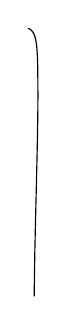
\begin{tikzpicture}[x=1mm,y=1mm,line cap=round]
\draw[line width=.42pt] (0,34)..controls(1.1,33.6)and(1.2,31.8)..(1.22,27)
  ..controls(1.3,21)and(.8,8)..(.76,0);
\end{tikzpicture}}\endgroup}
\end{GelfandAdjacentEvidence}



\Needspace{7\baselineskip}
\begin{GelfandAdjacentEvidence}{GELFAND-P000468}{1}
\SourcePage{GELFAND-P000468}{unlabelled}
\underline{13/\mbox{$\overline{\underline{\mathrm{XI}}}$}-72.}
\quad\underline{Gelfand sem..}

\underline{L. Vaserstein.}

\uuline{\mbox{$A$}} — assoc. ring (not necessarily with $1$).

\uuline{\mbox{$iA$}} — ring with a formally adjoined unit.

$iA/A=\mathbb Z$,\quad $A$ — two-sided ideal in $iA$.

$GA$ — mult. group of the ring.

$GA\subset A$

$(a,b)\longrightarrow a+b+ab$\qquad This is a binary assoc. oper.
\[
\Vert\qquad (e+a)(e+b)-e=a+b+ab
\]
\sout{\mbox{$iA$}}\quad \uuline{\mbox{$GA$}} — set of invertible elements with respect to this operation.
\Unclear{GELFAND-P000468}{initial-cancel}{The short crossed-out entry before $GA$ may read $iA$.}
\end{GelfandAdjacentEvidence}
\begin{GelfandAdjacentEvidence}{GELFAND-P000468}{2}


\[
a\longrightarrow1+a,\qquad A\longrightarrow1+A
\]
\uwave{homomorphism}.\quad
\begin{tabular}[t]{@{}l@{}}
\underline{into the ordinary}\\
\underline{invert. elems}.
\end{tabular}

\[
\begin{gathered}
f:A\longrightarrow B\\
f(GA)\subset GB
\end{gathered}
\]
\Unclear{GELFAND-P000468}{image-containment}{The sign before $GB$ is overwritten. It is provisionally set as $\subset$.}
\end{GelfandAdjacentEvidence}
\begin{GelfandAdjacentEvidence}{GELFAND-P000468}{3}


$i,G$ — functors to the cat. of rings with $1$ and the cat. of groups.

\uuline{\mbox{$M_kA$}} — matrices $k\times k$ with ordinary multiplication.

\uuline{\mbox{$\widetilde\Omega A$}}$=\{a=(a_{ij})\}$,
in $\forall$ row and column a finite no. of elems. $\ne0$,
(this is a ring)

\uuline{\mbox{$MA$}} — subring of finite matrices (a finite number of elems. $\ne0$).
(two-sided ideal in $\widetilde\Omega A$).

\uuline{\mbox{$\Omega A$}}$=\widetilde\Omega A/MA$
\Unclear{GELFAND-P000468}{omega-letter}{The letter before $A$ on the left is overwritten. It reads $\Omega$.}
\end{GelfandAdjacentEvidence}
\begin{GelfandAdjacentEvidence}{GELFAND-P000468}{4}


$M,\widetilde\Omega,\Omega$ — functors.

\[
\underset{\vert}{\text{\uuline{\mbox{$\Theta A$}}}}\subset MA
\]
upper triangular $a=(a_{ij})$:\quad $a_{ij}=0$ when $i\le j$ \sout{\ldots}
\SourceFigure{GELFAND-P000468}{theta-link}{A short vertical stroke is drawn below the double underline under $\Theta A$.}
\end{GelfandAdjacentEvidence}
\begin{GelfandAdjacentEvidence}{GELFAND-P000468}{5}

\Unclear{GELFAND-P000468}{triangular-convention}{The manuscript has “upper triangular” and $a_{ij}=0$ when $i\le j$.}
\end{GelfandAdjacentEvidence}
\begin{GelfandAdjacentEvidence}{GELFAND-P000468}{6}

\Incomplete{GELFAND-P000468}{cancel-inequality}{Several signs one above another are crossed out after the inequality.}
\end{GelfandAdjacentEvidence}
\begin{GelfandAdjacentEvidence}{GELFAND-P000468}{7}


\underline{Remark}. If $N\xrightarrow{\sim}N$ is a bijection, there is a map of the matrix ring
(\sout{th.} autom.) — simultaneous perm. of rows and columns.
\Unclear{GELFAND-P000468}{cancel-auto}{The crossed-out abbreviation before “autom.” may read «эт».}
\end{GelfandAdjacentEvidence}
\begin{GelfandAdjacentEvidence}{GELFAND-P000468}{8}

(inner autom. perm. of rows and columns)
\Unclear{GELFAND-P000468}{inner-ambient}{The parenthesis reads «внутр. автом.» (“inner autom.”).}
\end{GelfandAdjacentEvidence}
\begin{GelfandAdjacentEvidence}{GELFAND-P000468}{9}


Even if $N\longrightarrow N$ is any map, it is assigned an \underline{endomorphism}.
\Unclear{GELFAND-P000468}{next-word}{The first word reads «Даже» (“even”).}
\end{GelfandAdjacentEvidence}
\begin{GelfandAdjacentEvidence}{GELFAND-P000468}{10}

\Unclear{GELFAND-P000468}{arbitrary-reindexing}{The last word is underlined and reads “endomorphism.”}
\end{GelfandAdjacentEvidence}
\begin{GelfandAdjacentEvidence}{GELFAND-P000468}{11}


$GMA$ — mult. group, $MA$,\quad $GMA\subset MA$.

\uwave{Simplicial structure in \mbox{$MA$}.}

$X\subset GMA$ is called a simplex, if by a left shift and conjugation by a permutation matrix it can be taken into $\Theta A$
\Unclear{GELFAND-P000468}{left-shift-convention}{The manuscript reads «левым сдвигом» (“by a left shift”).}
\end{GelfandAdjacentEvidence}
\begin{GelfandAdjacentEvidence}{GELFAND-P000468}{12}


Note that $G\Theta A=\Theta A$ as a set (they are nilpotent)
\Unclear{GELFAND-P000468}{final-word}{The last letters are overwritten. The word reads “nilpotent.”}
\end{GelfandAdjacentEvidence}



\Needspace{7\baselineskip}
\begin{GelfandAdjacentEvidence}{GELFAND-P000469}{1}
\SourcePage{GELFAND-P000469}{unlabelled}
\Incomplete{GELFAND-P000469}{top-cancelled}{A crossed-out mark before the first line with a short stroke to its right. The reading is unresolved.}
\end{GelfandAdjacentEvidence}
\begin{GelfandAdjacentEvidence}{GELFAND-P000469}{2}

In fact
\SourceFigure{GELFAND-P000469}{inclusion-bracket}{The line under the inclusion turns up at both ends.\par\smallskip\centering
\begingroup\color{black}\GelfandFitDiagram{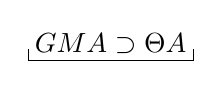
\begin{tikzpicture}
\node[inner sep=2.2pt] (inclusion) at (0,0) {$GMA\supset\Theta A$};
\draw (inclusion.south west) ++(0,4pt) -- (inclusion.south west) -- (inclusion.south east) -- ++(0,4pt);
\end{tikzpicture}}\endgroup}
\end{GelfandAdjacentEvidence}
\begin{GelfandAdjacentEvidence}{GELFAND-P000469}{3}


\uline{Mark the vertex \mbox{$0$}} — the identity of the group $GMA$.

\uuline{\mbox{$SA$}} — the corresponding simplicial scheme.

(Historical remark: Volodin used $SA$ to define the functors $K_{\mathbb C}^{n}$)
\par in essence
\Unclear{GELFAND-P000469}{top-functor-index}{The subscript reads $\mathbb C$, with an extra stroke inside the letter.}
\end{GelfandAdjacentEvidence}
\begin{GelfandAdjacentEvidence}{GELFAND-P000469}{4}


{\centering\rule{2.7em}{.4pt}\quad\textperiodcentered\quad\rule{3.1em}{.4pt}\par}
Suppose the ring $A$ has a unit. Then put.
\[
K_nA=\pi_{n-1}SA,\qquad n\geqslant1.
\]
For $n\geqslant2$ there is a group structure, commutative for $n\geqslant3$.

\uline{Another def. of the group structure (commutative).}

\uline{Whitehead's lemma}

Consider the spheroid $s\colon Z^n\longrightarrow SA$.
The group of permutations acts on $SA$ $f\colon N\longrightarrow N$.
We obtain a new spheroid $s^f$:
\SourceFigure{GELFAND-P000469}{spheroid-diagram}{The top arrow is unlabelled.\par\smallskip\centering
\begingroup\color{black}\GelfandFitDiagram{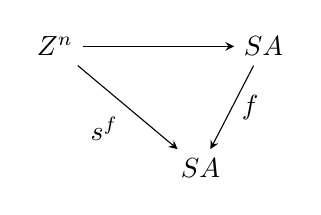
\begin{tikzpicture}[>=stealth]
\node (sphere) at (0,0) {$Z^n$};
\node (top) at (2.65,0) {$SA$};
\node (bottom) at (1.85,-1.55) {$SA$};
\draw[->] (sphere) -- (top);
\draw[->] (sphere) -- node[below left] {$s^f$} (bottom);
\draw[->] (top) -- node[right] {$f$} (bottom);
\end{tikzpicture}}\endgroup}
\end{GelfandAdjacentEvidence}
\begin{GelfandAdjacentEvidence}{GELFAND-P000469}{5}


They are always homotopic.

\uline{Idea of the proof:}

$\operatorname{Im}s\subset M_kA$.
\[
s=\left(\begin{array}{c|c}sz&0\\\hline 0&0\end{array}\right).
\]
Everything reduces to the case
\[
s^f=\left(\begin{array}{c|c}0&0\\\hline 0&sz\end{array}\right).
\]
\Unclear{GELFAND-P000469}{middle-block-argument}{The final sign in $sz$ has a cross-stroke and is provisionally set as a lowercase letter. Both matrices have two dividing rules.}
\end{GelfandAdjacentEvidence}
\begin{GelfandAdjacentEvidence}{GELFAND-P000469}{6}


($f$ of a special form: $fi=i+k$, we adjust it at $\infty$).

\[
\begin{pmatrix}a&0\\0&0\end{pmatrix}\quad
\begin{pmatrix}a&a\\0&0\end{pmatrix}\quad
\begin{pmatrix}0&a\\-1&0\end{pmatrix}\quad
\begin{pmatrix}0&0\\-1&a\end{pmatrix}\quad
\begin{pmatrix}0&0\\0&a\end{pmatrix}
\]
\Unclear{GELFAND-P000469}{five-spheroids}{The upper left zero in the third matrix is heavily retraced.}
\end{GelfandAdjacentEvidence}
\begin{GelfandAdjacentEvidence}{GELFAND-P000469}{7}

These are 5 spheroids. This is a homotopy. Each 2 neighbours are elementarily homotopic:

\[
s_1,s_2\colon S'\longrightarrow S'
\]
are called elem. homotopic if $\forall$ simplices $X\subset S$, $s_1X\cup s_2X$
is a simplex in $S'$.
\Unclear{GELFAND-P000469}{homotopy-domain}{A short stroke is visible above the first $S$. The next line has $X\subset S$ without a prime.}
\end{GelfandAdjacentEvidence}
\begin{GelfandAdjacentEvidence}{GELFAND-P000469}{8}


Let all $a$ lie in one simplex $X$.
Then $\begin{pmatrix}a&0\\0&0\end{pmatrix}$ and
$\begin{pmatrix}a&a\\0&0\end{pmatrix}$ lie in one simplex.

Let $a_0^{-1}\in X$. Multiply by $a_0$. Then they become upper triang.
If all $a$ are upper triangular, then all 5 matrices lie in one simplex.

{\centering\rule{3em}{.4pt}\quad\textperiodcentered\quad\rule{3.5em}{.4pt}\par}
\uline{The commutative group structure on \mbox{$K_nA$}.}
\[
MA\times MA\xrightarrow{\oplus}MA
\]
\[
\begin{array}{@{}ll|l@{}}
fi=2i & f,g\colon\mathbb N\longrightarrow\mathbb N & \text{noncommut., nonassoc., with no}\\
gi=2i+1 & a\oplus b=a^f+b^g & \text{identity elem.}
\end{array}
\]
\SourceFigure{GELFAND-P000469}{group-operation-margin}{A vertical rule separates the note about the operation.}
\end{GelfandAdjacentEvidence}
\begin{GelfandAdjacentEvidence}{GELFAND-P000469}{9}


\Unclear{GELFAND-P000469}{margin-left-bottom}{Outside the left edge of the text are a slanting stroke and a mark resembling a closing parenthesis. Their purpose is unresolved.}
\end{GelfandAdjacentEvidence}



\Needspace{7\baselineskip}
\begin{GelfandAdjacentEvidence}{GELFAND-P000470}{1}
\SourcePage{GELFAND-P000470}{unlabelled}
it induces the map $SA\times SA\longrightarrow SA$,
which gives operations on all $K_i$, $i\geqslant0$. (corr. verif. by Whitehead's lemma)
\Unclear{GELFAND-P000470}{whitehead-abbreviation}{The second abbreviation after «корр.» is provisionally read as «прв.».}
\end{GelfandAdjacentEvidence}
\begin{GelfandAdjacentEvidence}{GELFAND-P000470}{2}

They are commutative and agree with those introduced earlier by mutual distributivity, which is verified by Whitehead's lemma.

{\centering\rule{2em}{.4pt}\quad\textperiodcentered\quad\rule{3.4em}{.4pt}\par}
One can define a sum — $H$-space.
On $\widetilde\Omega A$ one can even add an inf. number of matrices!
Hence it will have trivial $K$-functors.
\Unclear{GELFAND-P000470}{omega-mark}{A long wavy mark is written over $\Omega$. It is set as $\widetilde\Omega$.}
\end{GelfandAdjacentEvidence}
\begin{GelfandAdjacentEvidence}{GELFAND-P000470}{3}


{\centering\rule{2.4em}{.4pt}\quad\textperiodcentered\quad\rule{3.1em}{.4pt}\par}
\uuline{\mbox{$K_1A=\pi_0SA$}.}

This is the set of connected components in $GMA$.

$EA$ — the connected component of the identity. (products of \(\underset{\substack{\vert\\\text{\scriptsize pseudotriangular}}}{\text{elem.}}\) matrices),
\SourceFigure{GELFAND-P000470}{pseudo-triangular-insertion}{“Pseudotriangular” is written under “elem.” and connected to it by a stroke.}
\end{GelfandAdjacentEvidence}
\begin{GelfandAdjacentEvidence}{GELFAND-P000470}{4}


\SourceFigure{GELFAND-P000470}{perfectness-hypotheses}{The stepped outline encloses both hypotheses. The arrow starts level with the first one.\par\smallskip\centering
\begingroup\color{black}\GelfandFitDiagram{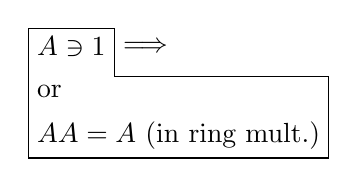
\begin{tikzpicture}[inner sep=3pt]
\node[anchor=west] (unit) at (0,0) {$A\ni1$};
\node[anchor=west] (alt) at (0,-.56) {or};
\node[anchor=west] (idem) at (0,-1.12) {$AA=A$ (in ring mult.)};
\draw (unit.north west) -- (unit.north east) |- (alt.north east -| idem.east)
      -- (idem.south east) -- (idem.south west) -- cycle;
\node[right] at (unit.east) {$\Longrightarrow$};
\end{tikzpicture}}\endgroup}
\end{GelfandAdjacentEvidence}
\begin{GelfandAdjacentEvidence}{GELFAND-P000470}{5}

\[
EA=[GMA,GMA]=[EA,EA].
\]

$K_2A$ — homot. classes of loops. Loops — relations of elem. matrices.

$\Theta A$ has generators $a^{ij}$
\Incomplete{GELFAND-P000470}{middle-generator-cancelled}{The entry after $a^{ij}$ is heavily crossed out. A short leftward arrow is visible below “Loops”.}
\end{GelfandAdjacentEvidence}
\begin{GelfandAdjacentEvidence}{GELFAND-P000470}{6}

(at position $i,j$ stands $a\in A$).

Relations: Steinberg
\[
\begin{gathered}
a^{ij}\ast b^{ij}=(a+b)^{ij},\\
[a^{ij},b^{jk}]=(ab)^{ik}
\end{gathered}
\]
and for some the commutator is $0$.

These are the defining relations.

Let $StA$ — be the group gen. by these generators and relations.
\[
0\longrightarrow K_2A\longrightarrow StA\longrightarrow EA\longrightarrow0
\]
\[
\begin{gathered}
\vert\\[-.2ex]
\text{homot. classes of paths from }0\text{ to somewhere}\\
\text{(with fixed start and end)}
\end{gathered}
\]
\SourceFigure{GELFAND-P000470}{steinberg-paths}{The annotation is connected by a vertical stroke to $StA$.}
\end{GelfandAdjacentEvidence}
\begin{GelfandAdjacentEvidence}{GELFAND-P000470}{7}


{\centering\rule{3.1em}{.4pt}\quad\textperiodcentered\quad\rule{4em}{.4pt}\par}
\Unclear{GELFAND-P000470}{lower-margin-mark}{There is a single retraced mark to the left of the formula. Its reading is unresolved.}
\end{GelfandAdjacentEvidence}
\begin{GelfandAdjacentEvidence}{GELFAND-P000470}{8}

\[
K_2A=\underset{\text{(group homology)}}{\underbrace{H_2EA}}\qquad\sim\qquad
StA=\text{the universal central extension of }EA.
\]

\uline{Problem:} suppose there are 3 matrices in $GMA$. All segments are simplices.
Then all 3 form a simplex.

Generalization: if any pair is a simplex, then all form a simplex.
(space of \uline{tolerance})

{\centering\rule{4em}{.4pt}\quad\textperiodcentered\quad\rule{2.3em}{.4pt}\par}
\uuline{D. A. Kazhdan.}\qquad\uline{Derived category.}

$C$ — an abelian category. Consider the category of complexes $K_C$.
\SourceFigure{GELFAND-P000470}{complexes-diagram}{The arrows point up in both columns. Two arrows point right between the columns.\par\smallskip\centering
\begingroup\color{black}\GelfandFitDiagram{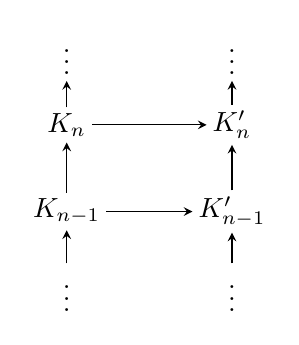
\begin{tikzpicture}[>=stealth,every node/.style={inner sep=2pt}]
\node (l0) at (0,0) {$\vdots$}; \node (r0) at (2.1,0) {$\vdots$};
\node (l1) at (0,-.9) {$K_n$}; \node (r1) at (2.1,-.9) {$K'_n$};
\node (l2) at (0,-2) {$K_{n-1}$}; \node (r2) at (2.1,-2) {$K'_{n-1}$};
\node (l3) at (0,-3) {$\vdots$}; \node (r3) at (2.1,-3) {$\vdots$};
\draw[->] (l1) -- (r1);
\draw[->] (l2) -- (r2);
\draw[->] (l1) -- (l0);
\draw[->] (l2) -- (l1);
\draw[->] (l3) -- (l2);
\draw[->] (r1) -- (r0);
\draw[->] (r2) -- (r1);
\draw[->] (r3) -- (r2);
\end{tikzpicture}}\endgroup}
\end{GelfandAdjacentEvidence}
\begin{GelfandAdjacentEvidence}{GELFAND-P000470}{9}


\Unclear{GELFAND-P000470}{bottom-cancelled-words}{A fragment before “with morphisms” is struck out. A possible reading is «с сост. об.».}
\end{GelfandAdjacentEvidence}
\begin{GelfandAdjacentEvidence}{GELFAND-P000470}{10}

\uline{with morphisms \mbox{$f$} the homot. classes of morphisms of complexes.}
\Unclear{GELFAND-P000470}{bottom-right-cancelled}{A single mark after “morphisms” is struck out. Its reading is unresolved.}
\end{GelfandAdjacentEvidence}
\begin{GelfandAdjacentEvidence}{GELFAND-P000470}{11}

\SourceFigure{GELFAND-P000470}{morphism-underline}{A continuous stepped underline runs beneath the two lines.}
\end{GelfandAdjacentEvidence}
\begin{GelfandAdjacentEvidence}{GELFAND-P000470}{12}


\[
\begin{gathered}
S\subset\operatorname{Hom}K_C\\[-.2ex]
\vert\\[-.2ex]
\text{morph. inducing an isomorphism of homologies}
\end{gathered}
\]
\SourceFigure{GELFAND-P000470}{homology-label}{The annotation is connected by a vertical stroke to $S$.}
\end{GelfandAdjacentEvidence}



\Needspace{7\baselineskip}
\begin{GelfandAdjacentEvidence}{GELFAND-P000471}{1}
\SourcePage{GELFAND-P000471}{unlabelled}
\uline{Lemma}. Let $f;g\colon K\longrightarrow K'$ be two morphisms.
\Unclear{GELFAND-P000471}{lemma-delimiter}{Two strokes appear between $f$ and $g$, here set as a semicolon.}
\end{GelfandAdjacentEvidence}
\begin{GelfandAdjacentEvidence}{GELFAND-P000471}{2}


The following statements are equivalent:

$1^\circ$. $\exists K_1$, $s_1\in S$:
\SourceFigure{GELFAND-P000471}{lemma-precomposition}{The first diagram with the equality written below it.\par\smallskip\centering
\begingroup\color{black}\GelfandFitDiagram{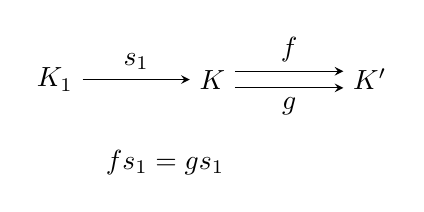
\begin{tikzpicture}[>=stealth]
\node (start) at (0,0) {$K_1$};
\node (middle) at (2,0) {$K$};
\node (end) at (4,0) {$K'$};
\draw[->] (start) -- node[above] {$s_1$} (middle);
\draw[->] ([yshift=3pt]middle.east) -- node[above] {$f$} ([yshift=3pt]end.west);
\draw[->] ([yshift=-3pt]middle.east) -- node[below] {$g$} ([yshift=-3pt]end.west);
\node at (1.4,-1.05) {$fs_1=gs_1$};
\end{tikzpicture}}\endgroup}
\end{GelfandAdjacentEvidence}
\begin{GelfandAdjacentEvidence}{GELFAND-P000471}{3}


$2^\circ$. $\exists K_2$, $s_2\in S$
\SourceFigure{GELFAND-P000471}{lemma-postcomposition}{The second diagram with the equality written below it.\par\smallskip\centering
\begingroup\color{black}\GelfandFitDiagram{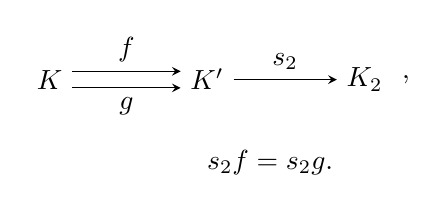
\begin{tikzpicture}[>=stealth]
\node (start) at (0,0) {$K$};
\node (middle) at (2,0) {$K'$};
\node (end) at (4,0) {$K_2$};
\draw[->] ([yshift=3pt]start.east) -- node[above] {$f$} ([yshift=3pt]middle.west);
\draw[->] ([yshift=-3pt]start.east) -- node[below] {$g$} ([yshift=-3pt]middle.west);
\draw[->] (middle) -- node[above] {$s_2$} (end);
\node[right] at (end.east) {,};
\node at (2.8,-1.05) {$s_2f=s_2g$.};
\end{tikzpicture}}\endgroup}
\end{GelfandAdjacentEvidence}
\begin{GelfandAdjacentEvidence}{GELFAND-P000471}{4}


{\centering\rule{3em}{.4pt}\quad\textperiodcentered\quad\rule{3.4em}{.4pt}\par}
$L_C$ — the same objects, and the morphisms: \uline{allow inverting \mbox{$s^{-1}$} and}
\par\hspace*{3em}\uline{Ore relations.}
\SourceFigure{GELFAND-P000471}{ore-insertion}{“Ore relations” is written below the first line, with a stepped rule.}
\end{GelfandAdjacentEvidence}
\begin{GelfandAdjacentEvidence}{GELFAND-P000471}{5}

The lemma makes it poss. to define the product correctly.
\Unclear{GELFAND-P000471}{product-reading}{The manuscript has «возможно» immediately before «корректно».}
\end{GelfandAdjacentEvidence}
\begin{GelfandAdjacentEvidence}{GELFAND-P000471}{6}


{\centering\rule{3em}{.4pt}\quad\textperiodcentered\quad\rule{3.5em}{.4pt}\par}
\(\overset{\scriptstyle +}{\text{See}}\)\quad\uline{Hartshorne}. Residues and duality.
\Unclear{GELFAND-P000471}{middle-reference-mark}{A short cross-shaped mark appears above «См.» (“See”).}
\end{GelfandAdjacentEvidence}
\begin{GelfandAdjacentEvidence}{GELFAND-P000471}{7}


{\centering\rule{3.9em}{.4pt}\quad\textperiodcentered\quad\rule{3.4em}{.4pt}\par}
\uuline{V. Buchstaber.}

\begin{tabular}{@{}llll@{}}
References: & C.–E. & 213--223 & (Cartan and Eilenberg)\\
 & M. & 358--370 & (Mac Lane)\\
 & Adams & Mat. $3\colon4$ & pp. 7--19.
\end{tabular}
\Unclear{GELFAND-P000471}{middle-maclane}{The parenthesis reads «Маклейн» (“Mac Lane”).}
\end{GelfandAdjacentEvidence}
\begin{GelfandAdjacentEvidence}{GELFAND-P000471}{8}


{\centering\rule{2.8em}{.4pt}\quad\textperiodcentered\quad\rule{3em}{.4pt}\par}
\[
A=\sum_{n\geqslant0}A_n\qquad\text{— grad. ring.}
\]
$A_n$ — an $A_0$-module for every $n\geqslant0$.
\[
0\longleftarrow A_0\xleftarrow{\varepsilon}A
\longleftarrow C_1\longleftarrow C_2\longleftarrow\cdots
\longleftarrow C_s\xleftarrow{d_{s+1}}C_{s+1}\longleftarrow\cdots
\]
($\varepsilon$ assigns $A$ zeroth comp. to each $a\in A$).
\Unclear{GELFAND-P000471}{lower-augmentation-a}{A separate $A$ is written immediately after «сопост.» (“assigns”).}
\end{GelfandAdjacentEvidence}
\begin{GelfandAdjacentEvidence}{GELFAND-P000471}{9}


Complete to a \uwave{grad. free resolution}.

The functor $\operatorname{Hom}_A(\cdot,A_0)$. takes $d_s$ to $(d_s)^*$.
\Unclear{GELFAND-P000471}{lower-hom-coefficient}{A small zero is visible below and to the right of the second argument $A$, against the parenthesis.}
\end{GelfandAdjacentEvidence}
\begin{GelfandAdjacentEvidence}{GELFAND-P000471}{10}

\[
H^s(A)=\operatorname{Ker}(d_{s+1})^*/\operatorname{Im}(d_s)^*
\]
\SourceFigure{GELFAND-P000471}{cohomology-index}{The numerator has $d_{s+1}$ and the denominator $d_s$.}
\end{GelfandAdjacentEvidence}


\uline{Theorem:}\quad 1) A free resolution exists

\hspace*{6em}2) The groups $H^s(A)$ are independent of the resolution.

\[
H(A)=\sum_{s=0}^{\infty}H^s(A)\qquad\text{— a graded ring.}
\]
A def. will be given for the multiplication of \uline{Yoneda}.
\[
\begin{gathered}
f\in H^i(A),\quad g\in H^j(A),\quad fg\in H^{i+j}(A),\\
\widetilde f\colon C_i\longrightarrow A_0;\qquad
\widetilde g\colon C_j\longrightarrow A_0.
\end{gathered}
\]


\Needspace{7\baselineskip}
\begin{GelfandAdjacentEvidence}{GELFAND-P000472}{1}
\SourcePage{GELFAND-P000472}{unlabelled}
\SourceFigure{GELFAND-P000472}{top-product-diagram}{The node $C_1$ is heavily retraced. The arrow from $C_i$ to $A$ is dashed, and the arrow from $C_{i+j}$ to $C_j$ has a single break.\par\smallskip\centering
\begingroup\color{black}\GelfandFitDiagram{\begin{tikzpicture}[>=stealth]
\node (ci) at (1.5,1.8) {$C_i$};
\node (topdots) at (3.15,1.8) {$\cdots$};
\node at (5.1,1.8) {$\cdots$};
\node (cij) at (6.7,1.8) {$C_{i+j}$};
\node (a0) at (0,0) {$A_0$};
\node (a) at (1.5,0) {$A$};
\node (c1) at (3.1,0) {$C_1$};
\node (dots) at (4.65,0) {$\cdots$};
\node (cj) at (6.1,0) {$C_j$};
\node (out) at (6.1,-1.5) {$A_0$};
\draw[->] (topdots) -- (ci);
\draw[->] (cj) -- (dots);
\draw[->] (dots) -- (c1);
\draw[->] (c1) -- (a);
\draw[->] (a) -- (a0);
\draw[->] (ci) -- node[left] {$\widetilde f$} (a0);
\draw[->,densely dashed] (ci) -- (a);
\draw (cij.south) -- (6.44,1.03);
\draw[->] (6.38,.91) -- (cj.north);
\draw[->] (cj) -- node[left] {$\widetilde g$} (out);
\end{tikzpicture}}\endgroup}
\end{GelfandAdjacentEvidence}
\begin{GelfandAdjacentEvidence}{GELFAND-P000472}{2}


We have obtained a homomorphism $C_{i+j}\longrightarrow A_0$.
\Unclear{GELFAND-P000472}{homomorphism-verb}{The first word is read as «Получили» (“we have obtained”). Its last two letters run together.}
\end{GelfandAdjacentEvidence}
\begin{GelfandAdjacentEvidence}{GELFAND-P000472}{3}


This gives
\[
A\underset{\text{assigns}}{\rightsquigarrow}H(A)
\qquad\text{(a ring)}
\]
$H(A)$ is generally noncommutative (!) in a genuine sense.
The classification of multivalued groups rests on this.
\Unclear{GELFAND-P000472}{multivalued-groups}{The manuscript abbreviates “multivalued” as «многозн.».}
\end{GelfandAdjacentEvidence}
\begin{GelfandAdjacentEvidence}{GELFAND-P000472}{4}

(So far in topology only commut. rings have occurred — there one always has Hopf algebras).

\uline{Standard resolution or \mbox{$B$}-resolution.}
\[
\overline A=\sum_{n>0}A_n
\]
\[
C_1=A\underset{A_0}{\otimes}\overline A
\qquad\text{Henceforth }A_0\text{ is omitted}
\]
(The starting rings are commutative!)
\[
\begin{gathered}
C_s=A\otimes(\overline A)^s.\\
d_{s+1}\colon A\otimes(\overline A)^{s+1}
\longrightarrow A\otimes(\overline A)^s
\end{gathered}
\]
\[
\begin{aligned}
d_s\bigl(a_0[a_1|a_2|\ldots|a_s]\bigr)
={}&(-1)^{\varepsilon(0)}a_0a_1[a_2|\ldots a_s]\\
 &+\sum(-1)^{\varepsilon(n)}a_0[a_1|\ldots|a_na_{n+1}|\ldots a_s]
\end{aligned}
\]
\Unclear{GELFAND-P000472}{bar-differential-indices}{Two indices in the product are retraced. The reading is $a_na_{n+1}$.}
\end{GelfandAdjacentEvidence}
\begin{GelfandAdjacentEvidence}{GELFAND-P000472}{5}


$\varepsilon(n)$ — certain functions of the index,
\sout{For even grading \mbox{$\varepsilon(n)=n$}.}
\par\uline{\mbox{$\varepsilon(n)=n$}, if all elems. are even.}
\SourceFigure{GELFAND-P000472}{even-sign-cancellation}{The condition on even elements is added below the deleted line and set off by a rule.}
\end{GelfandAdjacentEvidence}
\begin{GelfandAdjacentEvidence}{GELFAND-P000472}{6}


\[
\operatorname{Hom}_A(C_s,A_0)\simeq(\overline A^{\,*})^s,
\qquad \overline A^{\,*}=\operatorname{Hom}_{A_0}(\overline A,A_0)
\]
\[
d_s^*\colon[\alpha_1|\alpha_2|\ldots|\alpha_{s-1}]
=\sum(-1)^{\varepsilon(n)}
[\alpha_1|\ldots|\overline\Delta\alpha_n|\ldots|\alpha_{s-1}].
\]
\[
\varepsilon(n)=n,\quad\text{if }\deg\alpha_i=2k_i
\]

\uline{Def. \mbox{$\overline\Delta$}.}
\SourceFigure{GELFAND-P000472}{lower-coproduct-box}{The top arrow has a clear right head. Its retraced left end also resembles a head.\par\smallskip\centering
\begingroup\color{black}\GelfandFitDiagram{\begin{tikzpicture}[>=stealth,inner sep=2pt]
\node (tensor) at (2.1,0) {$A\underset{A_0}{\otimes}A$};
\node (alg) at (5.12,0) {$A$};
\draw[->,line width=1.1pt] ([yshift=4pt]tensor.east) -- (alg.west);
\draw[line width=.55pt] ([xshift=4pt,yshift=7pt]tensor.east)
  -- ([yshift=4pt]tensor.east) -- ([xshift=4pt,yshift=1pt]tensor.east);
\node at (4.25,-.52) {$\mu$ (mult.)};
\node (tdual) at (2.1,-1.25) {$A^*\underset{A_0}{\otimes}A^*$};
\node (dual) at (5.12,-1.25) {$A^*$};
\draw[->] (dual) -- ([yshift=3pt]tdual.east);
\node at (6.37,-1.25) {$\colon\quad\Delta$};
\node at (7.16,-1.82) {dual to $\mu$};
\node (reduced) at (2.2,-2.55) {$a\otimes1+1\otimes a+\overline\Delta a$};
\node (arg) at (5.12,-2.55) {$a$};
\draw[->] (arg) -- (reduced);
\node at (8.05,-2.55) {(Def. $\overline\Delta$)};
\draw (.58,.56) -- (7.32,.56) -- (7.32,-1.48) -- (9.67,-1.48)
      -- (9.67,-3.02) -- (-.22,-3.02) -- (-.22,-1.35)
      -- (.58,-1.08) -- cycle;
\end{tikzpicture}}\endgroup}
\end{GelfandAdjacentEvidence}
\begin{GelfandAdjacentEvidence}{GELFAND-P000472}{7}


In fact
\[
\operatorname{Im}\overline\Delta\subset\overline{A^*}.
\]
\Unclear{GELFAND-P000472}{lower-reduced-image}{The bar on the right extends over both $A$ and the star.}
\end{GelfandAdjacentEvidence}
\begin{GelfandAdjacentEvidence}{GELFAND-P000472}{8}


This gives another definition of multiplication,
\[
\begin{aligned}
C_s^*&\qquad f=[\alpha_1|\ldots|\alpha_s]\\
C_{s'}^*&\qquad g=[\alpha'_1|\ldots|\alpha'_{s'}]
\end{aligned}
\qquad
f\cdot g=[\alpha_1|\ldots|\alpha_s|\alpha'_1|\ldots|\alpha'_{s'}]
\]
\Unclear{GELFAND-P000472}{bottom-prime-index}{The last index in $g$ reads $s^{\prime}$. The separator after the first primed term in the product is heavily retraced.}
\end{GelfandAdjacentEvidence}



\Needspace{7\baselineskip}
\begin{GelfandAdjacentEvidence}{GELFAND-P000473}{1}
\SourcePage{GELFAND-P000473}{unlabelled}
\uline{20/\mbox{$\overline{\underline{\mathrm{XI}}}$}-72.}
\qquad\uline{Gelfand sem..}

\uuline{Kostyuchenko.}\qquad\uuline{One example.}
\SourceFigure{GELFAND-P000473}{date-heading}{The month is given as a Roman numeral. The name and title are double-underlined.}
\end{GelfandAdjacentEvidence}
\begin{GelfandAdjacentEvidence}{GELFAND-P000473}{2}

\[
\begin{gathered}
v''+2a\lambda v'+b\lambda^2v=0\\
v(0)=v(\pi)=0.
\end{gathered}
\qquad\text{in }L_2[0,\pi].
\]

\SourceFigure{GELFAND-P000473}{pde-bracket}{A line under the equation turns up at both ends.\par\smallskip\centering
\begingroup\color{black}\GelfandFitDiagram{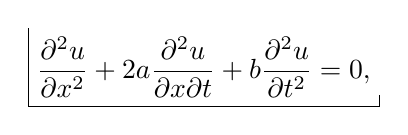
\begin{tikzpicture}
\node[inner sep=3pt] (pde) at (0,0)
  {$\displaystyle\frac{\partial^2u}{\partial x^2}
    +2a\frac{\partial^2u}{\partial x\partial t}
    +b\frac{\partial^2u}{\partial t^2}=0,$};
\draw (pde.north west) -- (pde.south west) -- (pde.south east) -- ++(0,4pt);
\end{tikzpicture}}\endgroup}
\end{GelfandAdjacentEvidence}
\begin{GelfandAdjacentEvidence}{GELFAND-P000473}{3}

\[
\begin{gathered}
0<x<\pi\\
0\leqslant t<+\infty
\end{gathered}
\]
\Unclear{GELFAND-P000473}{top-time-inequality}{The second inequality sign is retraced. The provisional reading is $0\leqslant t<+\infty$.}
\end{GelfandAdjacentEvidence}
\begin{GelfandAdjacentEvidence}{GELFAND-P000473}{4}

\uline{Suppose the eq. is elliptic.}
\Unclear{GELFAND-P000473}{elliptic-heading}{The first word reads «Пусть» (“Suppose”).}
\end{GelfandAdjacentEvidence}
\begin{GelfandAdjacentEvidence}{GELFAND-P000473}{5}


\[
\underline{a^2<b};\qquad\underline{b>0}.
\]
\[
v_k(x)=e^{\gamma kx}\sin kx,\qquad
\gamma=\frac{-a}{\sqrt{b-a^2}};\qquad k=\pm1,\ \pm2,\ \ldots .
\]
\SourceFigure{GELFAND-P000473}{gamma-bracket}{A rule with upturned ends is drawn below the formula for $\gamma$.}
\end{GelfandAdjacentEvidence}
\begin{GelfandAdjacentEvidence}{GELFAND-P000473}{6}


1. The system is complete, but it is unknown how to find the coefficients.
This is the question of finding the biorthog. system.
\Unclear{GELFAND-P000473}{upper-system-correction}{The end of “system” is retraced. A separate mark is crossed out after the period.}
\end{GelfandAdjacentEvidence}
\begin{GelfandAdjacentEvidence}{GELFAND-P000473}{7}

(found in terms of the inverse fn. of the Christoffel–Schwarz integral)

(\uline{a biorthog. system exists})

2. \uline{This is not a basis!} (not every vector expands into a conv. series in this system)

\sout{Even}\quad\uline{Moreover:} if there is an expansion in $L^2$,
then the limit — an analytic fn.! — and satisfies inf. many boundary conditions (the converse holds too).
\Unclear{GELFAND-P000473}{middle-cancelled-even}{The crossed-out word may read «Даже» (“Even”).}
\end{GelfandAdjacentEvidence}
\begin{GelfandAdjacentEvidence}{GELFAND-P000473}{8}


It cannot be summed by the Abel method of the first order.

\uline{if}
\[
\sum_{\lambda_k>0}e_k e^{\lambda_k t}v_k(x)
\]
\Unclear{GELFAND-P000473}{middle-abel-coefficient}{The coefficient is heavily retraced. The provisional reading is $e_k$.}
\end{GelfandAdjacentEvidence}
\begin{GelfandAdjacentEvidence}{GELFAND-P000473}{9}

\Incomplete{GELFAND-P000473}{middle-abel-cancelled}{Two short entries after $v_k(x)$ are heavily struck out. Their readings are unresolved.}
\end{GelfandAdjacentEvidence}
\begin{GelfandAdjacentEvidence}{GELFAND-P000473}{10}

has a limit as $t\to0$,
then the \uwave{limiting fn.} is analytic.
\SourceFigure{GELFAND-P000473}{limiting-function-line}{A wavy stroke runs above “fn.” and below “limiting”.}
\end{GelfandAdjacentEvidence}
\begin{GelfandAdjacentEvidence}{GELFAND-P000473}{11}


(Discrediting the Fourier method for the elliptic eq.)

With certain nonseparated conditions one can solve it.
\Unclear{GELFAND-P000473}{boundary-abbreviation}{The adjective before “conditions” is abbreviated as «неразд.».}
\end{GelfandAdjacentEvidence}
\begin{GelfandAdjacentEvidence}{GELFAND-P000473}{12}


\Incomplete{GELFAND-P000473}{lower-cancelled-marks}{Two marks before “Reason” are crossed out. Their readings are unresolved.}
\end{GelfandAdjacentEvidence}
\begin{GelfandAdjacentEvidence}{GELFAND-P000473}{13}

\uline{Reason for the poor behav.:} the resolvent grows $\exp$ in the angles
\SourceFigure{GELFAND-P000473}{resolvent-angle-diagram}{Two intersecting lines, broken strokes on the left, a dot at their crossing, and a circle and arrow on the right.\par\smallskip\centering
\begingroup\color{black}\GelfandFitDiagram{\begin{tikzpicture}[>=stealth]
\draw (-2.15,.35) -- (1.41,-.27);
\draw (-1.84,-.6) -- (1.51,.37);
\draw[densely dotted] (-2.21,-.15) -- (-.91,.02);
\fill (0,0) circle (1.3pt);
\draw (.82,.035) ellipse (.065 and .025);
\draw[->] (1.14,.025) -- (1.76,.07);
\end{tikzpicture}}\endgroup}
\end{GelfandAdjacentEvidence}
\begin{GelfandAdjacentEvidence}{GELFAND-P000473}{14}


On $[0,\pi-\varepsilon]$ it is overdetermined.

On $[0,\pi+\varepsilon]$, $0<\varepsilon<\pi$ it remains complete !!! (I. Bernstein)
\Unclear{GELFAND-P000473}{epsilon-lower-bound}{The lower bound is heavily retraced and is provisionally set as zero.}
\end{GelfandAdjacentEvidence}


On $[0,2\pi]$ many orthog. fns. arise.

\uline{A problem in the theory of entire fns..}
\[
\int_0^\pi f(x)e^{\gamma kx}\sin kx\,dx=0
\quad\Longrightarrow\quad
F(\lambda)=\int_0^\pi f(x)e^{\gamma\lambda x}\sin\lambda x\,dx
\]
$F(\lambda)$ is an entire fn. of $\exp$ type. It is 0 at integer points
$F(n)=0$, $n>0$.

\uline{The specific features must be taken into account.}

On $[0,\pi-\varepsilon]$ the type and indicator diagram work.

Uniqueness — ?

It is unknown what happens if one replaces $k$ by $\lambda_k$.


\Needspace{7\baselineskip}
\begin{GelfandAdjacentEvidence}{GELFAND-P000474}{1}
\SourcePage{GELFAND-P000474}{unlabelled}
\uuline{I. M. Gelfand}\qquad\uuline{on Arnold's work.}
\SourceFigure{GELFAND-P000474}{gelfand-arnold-heading}{The name and topic are double-underlined.}
\end{GelfandAdjacentEvidence}
\begin{GelfandAdjacentEvidence}{GELFAND-P000474}{2}

\[
(\mathbb R^n,0)\longrightarrow(\mathbb R,0)
\]
$f(x)=0$ — hypersurf.

How does the hypersurf. behave in a neighbourhood of $0$ — ?

$f\in C^\infty$;\quad $f(0)=0$, $df(0)=0$. (crit. point).

(In fact consider $\mathbb C^n\longrightarrow\mathbb C$)

Equiv. hypersurfaces — differ by a change of variables
\[
(\mathbb R^n,0)\longrightarrow(\mathbb R^n,0)\qquad
\text{(diffeom.)}.
\]

\uline{Simple hypersurf.:}\qquad\uline{\mbox{$f(x)=0$}}

if one perturbs it, there will be finitely many orbits
in jets of order $N$ (the bound on the number of orbits does not depend on the index $N$).

Enumeration of the simple orbits:
\SourceFigure{GELFAND-P000474}{simple-chain-graphs}{Two chains are drawn at left. The lower chain forks at its end.\par\smallskip\centering
\begingroup\color{black}\GelfandFitDiagram{\begin{tikzpicture}[vertex/.style={circle,draw,inner sep=1.45pt}]
\node[vertex] (a0) at (0,0) {};
\node[vertex] (a1) at (.75,0) {};
\node[vertex] (a2) at (1.45,0) {};
\node[vertex] (a3) at (2.02,0) {};
\node[vertex] (a4) at (4.23,0) {};
\draw (a0)--(a1)--(a2)--(a3)--(2.49,0);
\node at (2.95,0) {$\cdots$};
\draw (3.66,0)--(a4);
\node[vertex] (d0) at (-.15,-.82) {};
\node[vertex] (d1) at (.62,-.82) {};
\node[vertex] (d2) at (4.15,-.82) {};
\node[vertex] (d3) at (4.54,-.55) {};
\node[vertex] (d4) at (4.54,-1.09) {};
\draw (d0)--(d1)--(1.26,-.82);
\node at (1.81,-.82) {$\cdots$};
\draw (3.44,-.82)--(d2)--(d3);
\draw (d2)--(d4);
\end{tikzpicture}}\endgroup}
\end{GelfandAdjacentEvidence}
\begin{GelfandAdjacentEvidence}{GELFAND-P000474}{3}

\SourceFigure{GELFAND-P000474}{exceptional-graphs}{The right-hand chain has a downward branch at the third vertex. Its last links are broken.\par\smallskip\centering
\begingroup\color{black}\GelfandFitDiagram{\begin{tikzpicture}[vertex/.style={circle,draw,inner sep=1.35pt}]
\node[vertex] (e0) at (0,0) {};
\node[vertex] (e1) at (.68,0) {};
\node[vertex] (e2) at (1.14,0) {};
\node[vertex] (e3) at (1.66,0) {};
\node[vertex] (e4) at (2.17,0) {};
\node[vertex] (e5) at (2.98,0) {};
\node[vertex] (e6) at (3.76,0) {};
\node[vertex] (e7) at (1.14,-.53) {};
\draw (e0)--(e1)--(e2)--(e3)--(e4);
\draw (e2)--(e7);
\draw[densely dotted] (e4)--(e5)--(e6);
\node[right] at (4.14,-.06) {$E_6,E_7$ and $E_8$};
\end{tikzpicture}}\endgroup}
\end{GelfandAdjacentEvidence}
\begin{GelfandAdjacentEvidence}{GELFAND-P000474}{4}


Next: Most orbits are simple (as a rule, the orbit is simple).
\Incomplete{GELFAND-P000474}{middle-parenthetic-cancelled}{A short fragment after the opening parenthesis is struck out. Its reading is unresolved.}
\end{GelfandAdjacentEvidence}
\begin{GelfandAdjacentEvidence}{GELFAND-P000474}{5}

\uline{Nonsimple ones of codimension 6.}

\[
x_1^{n+1}+x_2^2+\cdots\,\ast=0
\]
— corr. to the first type.
\Unclear{GELFAND-P000474}{middle-simple-equation}{The first letter of the exponent $n+1$ is retraced. A separate star-like mark follows the ellipsis. A rule with upturned ends is drawn below the formula.}
\end{GelfandAdjacentEvidence}
\begin{GelfandAdjacentEvidence}{GELFAND-P000474}{6}


\uline{Versal deformation.}
\[
\begin{gathered}
F(x,\lambda)=0,\qquad F(x,0)=f(x),\\
\lambda=(\lambda_1,\lambda_2,\ldots,\lambda_k)
\end{gathered}
\]
Every other def. is equiv. to a def. induced from this one as follows:
\[
G(x,\mu)=F(X(x,\mu),\Psi(\mu))
\quad\text{and}\quad X(y,0)=y,\quad\Psi(0)=0
\]
\Unclear{GELFAND-P000474}{middle-induced-variables}{The first arguments of $G$ and $X$ are heavily retraced and provisionally read as $x$. The right side clearly has $X(y,0)=y$.}
\end{GelfandAdjacentEvidence}
\begin{GelfandAdjacentEvidence}{GELFAND-P000474}{7}


\uline{Rule for constructing a vers. family:}
Take an orbit and a set transverse to the orbit.
\SourceFigure{GELFAND-P000474}{transverse-sketch}{A curved line and a short transverse segment with a point at their intersection.\par\smallskip\centering
\begingroup\color{black}\GelfandFitDiagram{\begin{tikzpicture}
\draw (-.81,-.58) .. controls (-.36,.06) and (.03,.33) .. (.94,.59);
\draw[line width=.95pt] (-.39,.3) .. controls (-.12,.11) and (-.03,-.03) .. (.04,-.22);
\fill (-.11,.12) circle (1.5pt);
\end{tikzpicture}}\endgroup}
\end{GelfandAdjacentEvidence}
\begin{GelfandAdjacentEvidence}{GELFAND-P000474}{8}

{\centering\rule{1.8em}{.4pt}\quad\textperiodcentered\quad\rule{2.4em}{.4pt}\par}

\[
F(x,\lambda)=f(x)+
\sum a_i\left.\frac{\partial F}{\partial\lambda_i}\right|_{\lambda_i=0}
=f(x)+\sum c_i\varphi_i(x)+O(\lambda^2).
\]
\Unclear{GELFAND-P000474}{lower-taylor-coefficient}{The multiplier in the first sum is provisionally read as $a_i$. The evaluation subscript is $\lambda_i=0$.}
\end{GelfandAdjacentEvidence}
\begin{GelfandAdjacentEvidence}{GELFAND-P000474}{9}


\uuline{\mbox{$\varphi_i$} give}\quad\uline{an infinitesimal versal deformation:}
if $\forall$ fn. $a(x)$ is repr. in the form
\Unclear{GELFAND-P000474}{lower-definition-heading}{The first fragment is heavily retraced and double-underlined. The provisional reading is $\varphi_i$ «зад» (“give”).}
\end{GelfandAdjacentEvidence}
\begin{GelfandAdjacentEvidence}{GELFAND-P000474}{10}

\[
a(x)=\sum\underline{\underline{\frac{\partial f}{\partial x_i}}}\cdot h_i(x)
+\sum_{i=1}^{k}c_i\varphi_i(x)
\]
$a(x)$ defines an infinitesim. vers. deform.

($\varphi_i$ gen. the local ring of smooth maps)

\Incomplete{GELFAND-P000474}{bottom-cancelled-taylor}{A separate crossed-out entry precedes the parenthesis about Taylor expansion. Its reading is unresolved.}
\end{GelfandAdjacentEvidence}

(from the Taylor exp. of that fn.)

Important: the quotient ring by the \uline{Jacobian ideal}
$\left(\left\{\dfrac{\partial f}{\partial x_i}\right\}\right)$.

\uline{The quotient} — a finite-dimensional space of dimension $k$.

{\centering\rule{2.9em}{.4pt}\quad\textperiodcentered\quad\rule{3.4em}{.4pt}\par}


\Needspace{7\baselineskip}
\begin{GelfandAdjacentEvidence}{GELFAND-P000475}{1}
\SourcePage{GELFAND-P000475}{unlabelled}
\[
\underline{\underline{f=z_1^{k+1}+z_2^2+\cdots+z_n^2.}}
\]

Then
\[
\frac{\partial f}{\partial z_1}=z_1^k,\qquad
\frac{\partial f}{\partial z_2}=z_2,\ \ldots,
\]
\Unclear{GELFAND-P000475}{top-derivatives}{The right-hand sides are written as monomials without numerical factors.}
\end{GelfandAdjacentEvidence}
\begin{GelfandAdjacentEvidence}{GELFAND-P000475}{2}

hence the quotient ring is a space of dimension $k$.

\[
\varphi_i=1,z_i,z_i^2,\ldots,z_1^{k-1}
\]
\Unclear{GELFAND-P000475}{top-phi-indices}{The first two powers after $1$ have subscripts resembling $i$. The last has $1$.}
\end{GelfandAdjacentEvidence}
\begin{GelfandAdjacentEvidence}{GELFAND-P000475}{3}


Vers. deformation:
\[
\underline{\lambda_0+\lambda_1z_1+\cdots+\lambda_{k-1}z_1^{k-1}
+z_1^{k+1}+z^2}
\quad\text{— \uline{vers. deformation}}
\]
\SourceFigure{GELFAND-P000475}{versal-bracket}{A rule with upturned ends is drawn below the polynomial. The final term is written $z^2$.}
\end{GelfandAdjacentEvidence}
\begin{GelfandAdjacentEvidence}{GELFAND-P000475}{4}


{\centering\rule{2.8em}{.4pt}\quad\textperiodcentered\quad\rule{3.2em}{.4pt}\par}
\uline{\mbox{$F(z,\lambda)=0$}.}\qquad
The bifurc. diagram — the set of those $\lambda$, for which sing. points remain (in the vers. deformation).

\SourceFigure{GELFAND-P000475}{theorem-star}{Four segments meet at a common point to the left of the theorem.\par\smallskip\centering
\begingroup\color{black}\GelfandFitDiagram{\begin{tikzpicture}
\draw (-.72,.41)--(.64,-.58);
\draw (.05,.67)--(-.06,-.72);
\draw (-.96,-.27)--(.96,.16);
\draw (-1,-.62)--(.73,.46);
\end{tikzpicture}}\endgroup}
\end{GelfandAdjacentEvidence}
\begin{GelfandAdjacentEvidence}{GELFAND-P000475}{5}

\uuline{Thm.:} on an open
\(\underset{\text{\scriptsize\tikz[baseline=(label.base)]\node[draw,ellipse,inner sep=1pt] (label) {bifurc. diag.};}}{\text{set}}\)
the sing. points will already be simple (Morse).
\SourceFigure{GELFAND-P000475}{theorem-bifurcation-insertion}{“Bifurc. diag.” is written in a bubble below “set”.}
\end{GelfandAdjacentEvidence}
\begin{GelfandAdjacentEvidence}{GELFAND-P000475}{6}


\[
z_1^{k+1}+z_2^2=0
\qquad\Vert\qquad
\begin{gathered}
\text{the bifurc. diag. of this point —}\\[-.2ex]
\longrightarrow\text{ Swallowtail}.
\end{gathered}
\]
\[
\begin{gathered}
z_1^{k+1}+z_2^2+\lambda_{k-1}z_1^{k-1}+\cdots+\lambda_0\\
z_2^2=-p_{k+1}(z_1);\qquad z_2=\sqrt{-p_{k+1}(z_1)}.
\end{gathered}
\]
sing. points\quad $(z_2,P'(z_1))=0$, i.e.
\[
\underline{P(z_1)=0\ \text{and}\ P'(z_1)=0}
\]
($P$ has multiple roots)
\SourceFigure{GELFAND-P000475}{multiple-root-bracket}{A single rule with upturned ends surrounds the two equalities below.}
\end{GelfandAdjacentEvidence}
\begin{GelfandAdjacentEvidence}{GELFAND-P000475}{7}


Consider the complement of the bifurc. diagram and its fund. group.
It is the braid group of the Coxeter group.

Consider the eq.
\[
\underline{P(z,\lambda)=0,\quad |z|<\varepsilon}
\qquad\text{\uline{\mbox{$\lambda$} such that there are no singularities}}
\]
\Unclear{GELFAND-P000475}{middle-polynomial-name}{The first letter is heavily retraced. The provisional reading is $P$.}
\end{GelfandAdjacentEvidence}
\begin{GelfandAdjacentEvidence}{GELFAND-P000475}{8}


the homology of this space is $\ne0$ only in \sout{dim.}
\Incomplete{GELFAND-P000475}{lower-homology-cancelled}{Traces remain after the struck-out “dim.”. A full reading is unresolved.}
\end{GelfandAdjacentEvidence}
\begin{GelfandAdjacentEvidence}{GELFAND-P000475}{9}

half-dimension $n-1$.

It is a bouquet of $\mu$ spheres.
\SourceFigure{GELFAND-P000475}{sphere-bouquet}{Four loops with a common point depict the bouquet.\par\smallskip\centering
\begingroup\color{black}\GelfandFitDiagram{\begin{tikzpicture}
\draw (0,0) .. controls (-1.2,.83) and (-1.45,-.58) .. (0,0);
\draw (0,0) .. controls (-.37,1.37) and (.95,1.59) .. (0,0);
\draw (0,0) .. controls (1.7,1.32) and (1.7,-.86) .. (0,0);
\draw (0,0) .. controls (-.29,-1.73) and (-1.23,-1.45) .. (0,0);
\fill (0,0) circle (1.25pt);
\end{tikzpicture}}\endgroup}
\end{GelfandAdjacentEvidence}
\begin{GelfandAdjacentEvidence}{GELFAND-P000475}{10}


\Incomplete{GELFAND-P000475}{lower-left-cancelled}{The entry to the left of $H^{n-1}$ is heavily struck out. Its reading is unresolved.}
\end{GelfandAdjacentEvidence}
\begin{GelfandAdjacentEvidence}{GELFAND-P000475}{11}

$H^{n-1}$ has generators $e_1\ e_2\ldots\ e_\mu$.

The intersection index defines a scalar prod. $(e_i,e_k)$.

\[
n-1\equiv2\pmod4\qquad\Vert\qquad
\begin{gathered}
\text{neg. def.}\\
\text{semidef.}\\
\text{indef.}
\end{gathered}
\qquad\underline{e_i^2=-2}\quad\text{(always)}
\]
\Incomplete{GELFAND-P000475}{lower-signature-cancelled}{One line between “semidef.” and “indef.” is crossed out. Its reading is unresolved.}
\end{GelfandAdjacentEvidence}
\begin{GelfandAdjacentEvidence}{GELFAND-P000475}{12}


\uwave{monodromy}: rep. of the fund. gr. in
\Incomplete{GELFAND-P000475}{lower-monodromy-cancelled}{An entry after “in” is crossed out and followed by an ellipsis. Its reading is unresolved.}
\end{GelfandAdjacentEvidence}
\begin{GelfandAdjacentEvidence}{GELFAND-P000475}{13}

\ldots

{\centering\rule{4em}{1pt}\quad\textbullet\quad\rule{4em}{1pt}\par}

\sout{Atiyah}
\Unclear{GELFAND-P000475}{bottom-cancelled-name}{The struck-out name may read «Атья» (“Atiyah”).}
\end{GelfandAdjacentEvidence}

\uline{There are works by Atiyah, Bott,\ldots:} how to get rid of derivatives in Singer's calculations?
How can one study the topology of the world while sitting at one point? Finding explicit asymptotics for eqs. of the 2nd order (considerations of I. M. Gelfand, V. I. Arnold and others)

(will be in the next semester)

A. Shnirelman on Maslov's work.


\Needspace{7\baselineskip}
\begin{GelfandAdjacentEvidence}{GELFAND-P000476}{1}
\SourcePage{GELFAND-P000476}{unlabelled}
\uuline{V. M. Buchstaber.} (continuation).

\[
\begin{gathered}
A\overset{\text{addit.}}{=}\Lambda[[X]],\qquad
X_n\text{ — addit. generators}\\
X_n\cdot X_m=C_{n+m}^n X_{n+m}
\end{gathered}
\]
\Unclear{GELFAND-P000476}{additive-equality}{Two short parallel strokes under “addit.” read as an equals sign.}
\end{GelfandAdjacentEvidence}
\begin{GelfandAdjacentEvidence}{GELFAND-P000476}{2}


\[
\begin{gathered}
\operatorname{Ext}_A^{2,*}(\Lambda,\Lambda)\\[-.4ex]
\rotatebox[origin=c]{90}{$=$}\\[-.4ex]
\operatorname{Ker}d_3^*/\operatorname{Im}d_2^*
\end{gathered}
\qquad\text{in terms of the }B\text{-construction}
\]

$1^\circ$.
\[
d_3^*\colon\overline A^*\otimes\overline A^*
\longrightarrow\overline A^*\otimes\overline A^*\otimes\overline A^*
\]

\[
A^*=\operatorname{Hom}_{\Lambda}^{c}(\Lambda[[X]],\Lambda)
\overset{\text{add.}}{\simeq}\Lambda[x]
\]
\Unclear{GELFAND-P000476}{top-dual-hom}{The upper index of $\operatorname{Hom}$ reads $c$ and the lower one $\Lambda$.}
\end{GelfandAdjacentEvidence}
\begin{GelfandAdjacentEvidence}{GELFAND-P000476}{3}

\uuline{compact} (nonzero val. on a finite number).
\SourceFigure{GELFAND-P000476}{compact-annotation}{“Compact” is written below $\operatorname{Hom}$ and connected to it by a stroke.}
\end{GelfandAdjacentEvidence}
\begin{GelfandAdjacentEvidence}{GELFAND-P000476}{4}


\[
\begin{gathered}
\Delta\colon A^*\longrightarrow A^*\otimes A^*\\
\Delta x_n\longrightarrow x_n\otimes1+1\otimes x_n+\sum d_{i,j}x_i\otimes x_j^*
\end{gathered}
\]
\Unclear{GELFAND-P000476}{top-delta-star}{A star is visible after $x_j$. It is absent from the later formula for $\Delta x_n$.}
\end{GelfandAdjacentEvidence}
\begin{GelfandAdjacentEvidence}{GELFAND-P000476}{5}


\[
\begin{aligned}
(\Delta x_n,x_i\otimes x_j)&=d_{i,j}\\[-.4ex]
\qquad\rotatebox[origin=c]{90}{$=$}&\\[-.4ex]
(x_n,x_i\cdot x_j)&=(x_n,C_{i+j}^{i}x_{i+j})=C_{i+j}^{i}\delta_{n,i+j}
\end{aligned}
\]
\SourceFigure{GELFAND-P000476}{pairing-layout}{A vertical equals sign joins the two lines of the pairing.}
\end{GelfandAdjacentEvidence}
\begin{GelfandAdjacentEvidence}{GELFAND-P000476}{6}


\[
\Delta x_n=x_n\otimes1+1\otimes x_n+\sum C_n^i x_i\otimes x_{n-i}
\]
And put\quad $x_n=x^n$
\[
\begin{gathered}
\Delta x^n=(x\otimes1+1\otimes x)^n\\
d_3^*\colon \overline{\Lambda[x,y]}\longrightarrow\overline{\Lambda[x,y,z]}
\end{gathered}
\]

\[
d_3\Biggl(\underset{
  \substack{\rotatebox[origin=c]{90}{$=$}\\ \sum h_{i,j}x^iy^j}
}{h(x,y)}\Biggr)=\sum h_{ij}(\overline\Delta x^i)z^j
-\sum h_{i,j}x^i\overline\Delta y^j=
\]
\Unclear{GELFAND-P000476}{middle-differential-star}{The calculation has $d_3$ without a star before $h(x,y)$. The preceding line has $d_3^*$.}
\end{GelfandAdjacentEvidence}
\begin{GelfandAdjacentEvidence}{GELFAND-P000476}{7}


\[
\overline\Delta x^n=
\underset{\substack{
 \rotatebox[origin=c]{90}{$=$}\\
 (\Delta(x))^n\\
 \rotatebox[origin=c]{90}{$=$}\\
 (x+y)^n
}}{\Delta x^n}-x^n-y^n.
\]
\SourceFigure{GELFAND-P000476}{coproduct-identifications}{Below $\Delta x^n$, vertical equals signs connect $(\Delta(x))^n$ and $(x+y)^n$.}
\end{GelfandAdjacentEvidence}
\begin{GelfandAdjacentEvidence}{GELFAND-P000476}{8}


\[
=h(x+y,z)-\mbox{\sout{\ensuremath{h(x,z)}}}-h(y,z)
-h(x,y+z)+h(x,y)+\mbox{\sout{\ensuremath{h(x,z)}}}.
\]
\SourceFigure{GELFAND-P000476}{cancelled-cocycle-terms}{Both instances of $h(x,z)$ are crossed out. The minus and plus signs in front remain visible.}
\end{GelfandAdjacentEvidence}
\begin{GelfandAdjacentEvidence}{GELFAND-P000476}{9}


\uuline{\mbox{$\operatorname{Ker}d_3^*$}:}
\[
\boxed{h(x+y,z)+h(x,y)=h(x,y+z)+h(y,z)}
\]
Denote these cycles by $L$.
\SourceFigure{GELFAND-P000476}{kernel-relation-box}{The equality is enclosed in a rectangular box.}
\end{GelfandAdjacentEvidence}
\begin{GelfandAdjacentEvidence}{GELFAND-P000476}{10}


This is precisely the Lazard relation.
\Unclear{GELFAND-P000476}{lazard-name}{The adjective before “relation” reads «лазаровское» (“Lazard”).}
\end{GelfandAdjacentEvidence}


\[
\underline{\operatorname{Im}d_2^*}=\Lambda\{d_2^*x^n\}
\]
\[
0\longrightarrow\operatorname{Im}d_2^*\longrightarrow L
\longrightarrow\operatorname{Ext}_A^{2,n}(\Lambda,\Lambda)\longrightarrow0
\]

\uline{Calculation of the group \mbox{$\operatorname{Ext}$}.}

The eq. does not involve $\Lambda$. Hence it suffices to calc. 2 cases:

1)\quad $\Lambda$ — $Z_p$-module ($p$ — prime)

2)\quad $\Lambda=Q$


\Needspace{7\baselineskip}
\begin{GelfandAdjacentEvidence}{GELFAND-P000477}{1}
\SourcePage{GELFAND-P000477}{unlabelled}
there remains\quad $X_{p^i}$

\[
\underline{A=\widehat{\prod}\otimes A_i},\qquad
A_i=Z_p[X_{p^i}]/(X_{p^i}^p)\underset{Z_p}{\otimes}\Lambda
\]
\Unclear{GELFAND-P000477}{top-tensor-product}{The product sign has a hat. A tensor sign is written immediately to its right.}
\end{GelfandAdjacentEvidence}
\begin{GelfandAdjacentEvidence}{GELFAND-P000477}{2}


\[
\begin{gathered}
H^*(A_i)=\Lambda_p(u_i)\otimes Z_p[v_i],\qquad
\deg u_i=p^i,\quad\deg v_i=p^{i+1}\\
u_i\in\operatorname{Ext}^{1,p^i};\qquad
v_i\in\operatorname{Ext}^{2,p^{i+1}}
\end{gathered}
\]
\[
\operatorname{Ext}_A^{2,*}=
\left\{\underbrace{u_i u_j,\quad i<j,\quad v_k}_{\text{\uline{generators}}}\right\}.
\]
\Unclear{GELFAND-P000477}{top-generator-inequality}{The sign between $i$ and $j$ is heavily retraced. It is provisionally set as $i<j$.}
\end{GelfandAdjacentEvidence}
\begin{GelfandAdjacentEvidence}{GELFAND-P000477}{3}


\sout{This}\quad But:
symmetric ones are needed.\quad \uline{\mbox{$h(x,y)=h(y,x)$}}
\Unclear{GELFAND-P000477}{middle-cancelled-word}{The struck-out word before “But” may read «Это» (“This”).}
\end{GelfandAdjacentEvidence}
\begin{GelfandAdjacentEvidence}{GELFAND-P000477}{4}


\uuline{There are noncommut. one-dimensional groups!!}\qquad (if there is torsion)

(corr. to the cycles $u_i u_j$)

\uline{Example:}\quad $x+y+axy^p$, where $a^2=0$ \quad
over $Z_p[a]/(a^2)$.
\SourceFigure{GELFAND-P000477}{formal-group-law}{The term $axy^p$ and the condition $a^2=0$ occur on the same line.}
\end{GelfandAdjacentEvidence}
\begin{GelfandAdjacentEvidence}{GELFAND-P000477}{5}

This is a noncommut. formal group!!

There are as many of them as there are cycles.

$v_k$ corr. to commut. groups
\[
h(x,y)=(x+y)^{p^{k+1}}-x^{p^{k+1}}-y^{p^{k+1}}
\]
coeff. divisible by $p$ (only)
\Unclear{GELFAND-P000477}{bottom-divisibility-word}{The word in parentheses reads «только» (“only”).}
\end{GelfandAdjacentEvidence}
\begin{GelfandAdjacentEvidence}{GELFAND-P000477}{6}


\SourceFigure{GELFAND-P000477}{lazard-polynomial-bracket}{A rule with upturned ends is drawn below the formula.\par\smallskip\centering
\begingroup\color{black}\GelfandFitDiagram{\begin{tikzpicture}
\node[inner sep=3pt] (formula) at (0,0)
 {$\displaystyle L_{p^{k+1}}(x,y)=\frac{h(x,y)}{p}$};
\draw (formula.south west) ++(0,5pt) -- (formula.south west)
 -- (formula.south east) -- ++(0,5pt);
\end{tikzpicture}}\endgroup}
\end{GelfandAdjacentEvidence}
\begin{GelfandAdjacentEvidence}{GELFAND-P000477}{7}


\uline{(in \mbox{$\forall$} dimension one generator each)}

\uwave{That is all for this semester.}
\SourceFigure{GELFAND-P000477}{semester-ending}{The last line has both a wavy underline and a broken straight underline.}
\end{GelfandAdjacentEvidence}



\Needspace{7\baselineskip}
\begin{GelfandAdjacentEvidence}{GELFAND-P000478}{1}
\SourcePage{GELFAND-P000478}{unlabelled}
\uline{12/\mbox{$\overline{\underline{\mathrm{II}}}$}-73.}
\qquad\uline{Gelfand sem.}

\uline{Plan:}\quad 1. Buchstaber, Mishchenko: Topology (Sullivan's work)

\hspace*{3.5em}2. Works by Deligne and Langlands

\uline{V. Buchstaber.}\qquad\uline{On Sullivan's first paper.}

$M^n$ — manif.

A smoothing of $M^n$ — is a sm. manif. $N^n$ and a homot. equiv.
$N^n\xrightarrow{f}M^n$
\SourceFigure{GELFAND-P000478}{smoothings-diagram}{Three arrows connect the two smooth manifolds and their common target.\par\smallskip\centering
\begingroup\color{black}\GelfandFitDiagram{\begin{tikzpicture}[>=stealth]
\node (n1) at (0,0) {$N_1^n$};
\node (n2) at (0,-1.3) {$N_2^n$};
\node (m) at (2.35,0) {$M^n$};
\draw[->] (n1) -- node[above] {$f_1$} (m);
\draw[->] (n1) -- node[left] {$g$} (n2);
\draw[->] (n2) -- node[below right] {$f_2$} (m);
\end{tikzpicture}}\endgroup}
\end{GelfandAdjacentEvidence}
\begin{GelfandAdjacentEvidence}{GELFAND-P000478}{2}

Equiv. $\Longleftrightarrow\exists$ a diffeom. $g$, such that this square commutes (up to homotopy).

$S(M^n)$ — the set of classes of equiv. smoothings.

\Incomplete{GELFAND-P000478}{top-milnor-cancelled}{A short entry above “Milnor” is heavily crossed out. Its reading is unresolved.}
\end{GelfandAdjacentEvidence}
\begin{GelfandAdjacentEvidence}{GELFAND-P000478}{3}

\uline{Milnor:}\quad $\operatorname{Card}S'(S^7)=28$.
\Unclear{GELFAND-P000478}{milnor-cardinality}{A short stroke is visible between the first $S$ and the parenthesis. It is set as $S^{\prime}$.}
\end{GelfandAdjacentEvidence}
\begin{GelfandAdjacentEvidence}{GELFAND-P000478}{4}


Description of\quad $S(M^n)$ — ?

\uline{Sullivan} considers in $M^n$ a fixed piecewise-linear structure.
\par\hfill ($M^n$ — a polyhedron)

\uwave{and solved the prob. in this formulation:}

(in place of a diffeom. — a piecewise-lin.
\Incomplete{GELFAND-P000478}{middle-cancelled-homeo}{A heavily crossed-out entry follows “piecewise-lin.”. Its reading is unresolved.}
\end{GelfandAdjacentEvidence}
\begin{GelfandAdjacentEvidence}{GELFAND-P000478}{5}

homeomorphism)

Obtain\quad $PL(M^n)$.

Here always\quad\uuline{\mbox{$PL(S^n)=\{S^n\}$}}
— where the Poincaré prob. has been solved (for $n\geqslant5$).

Consider on $M^n$
\(\overset{\text{\scriptsize\tikz[baseline=(word.base)]\node[draw,ellipse,inner sep=1pt] (word) {Vect.};}}{\vphantom{x}}\)
a bundle $\xi$, stable (of large dim.).
\Incomplete{GELFAND-P000478}{middle-vector-cancelled}{The old entry before “bundle” is inked over. “Vect.” is inserted above it.}
\end{GelfandAdjacentEvidence}
\begin{GelfandAdjacentEvidence}{GELFAND-P000478}{6}


\sout{trivial in several degrees}
\Unclear{GELFAND-P000478}{middle-cancelled-phrase}{The struck-out phrase is provisionally read as «несколько степен. тривиальное».}
\end{GelfandAdjacentEvidence}
\begin{GelfandAdjacentEvidence}{GELFAND-P000478}{7}


$T_\xi$ — the Thom complex of the bundle $\xi$,
\SourceFigure{GELFAND-P000478}{thom-quotient-bracket}{The formula has a bottom rule with upturned ends.\par\smallskip\centering
\begingroup\color{black}\GelfandFitDiagram{\begin{tikzpicture}
\node[inner sep=3pt] (quotient) at (0,0) {$\displaystyle T_\xi=\frac{D(\xi)}{S(\xi)}$};
\draw (quotient.south west) ++(0,7pt) -- (quotient.south west)
 -- (quotient.south east) -- ++(0,7pt);
\end{tikzpicture}}\endgroup}
\end{GelfandAdjacentEvidence}
\begin{GelfandAdjacentEvidence}{GELFAND-P000478}{8}

\[
\begin{gathered}
D\text{ — bundle of balls},\\
S\text{ — bundle of spheres}.
\end{gathered}
\]

$\dim\xi=m$.
\[
\underset{\substack{\vert\\ \text{\uline{at a point.}}}}{S^m}
 \overset{i}{\subset}T_\xi
\]
\SourceFigure{GELFAND-P000478}{point-inclusion}{A stroke connects “at a point” to the left-hand sphere.}
\end{GelfandAdjacentEvidence}
\begin{GelfandAdjacentEvidence}{GELFAND-P000478}{9}

\SourceFigure{GELFAND-P000478}{bundle-fibre-diagram}{In the diagram at right, the point maps by inclusion into the base.\par\smallskip\centering
\begingroup\color{black}\GelfandFitDiagram{\begin{tikzpicture}[>=stealth]
\node (r) at (0,0) {$\mathbb R^m$};
\node (xi) at (1.85,0) {$\xi$};
\node (point) at (0,-1.25) {$*$};
\node (base) at (1.85,-1.25) {$M^n$};
\draw[->] (r) -- (xi);
\draw[->] (r) -- (point);
\draw[->] (xi) -- (base);
\draw[->] ([xshift=3pt]point.east) .. controls (.67,-1.05) and (.55,-1.25) .. (.81,-1.25) -- (base);
\end{tikzpicture}}\endgroup}
\end{GelfandAdjacentEvidence}
\begin{GelfandAdjacentEvidence}{GELFAND-P000478}{10}


The bundle $\xi$ is called $J$-trivial, if $\exists$ a map $\varphi$; such that

\SourceFigure{GELFAND-P000478}{lower-j-diagram}{The first arrow is labelled $i$. The mark at the right-hand sphere and the large crossed-out entry to its right remain unresolved. The arc from the left sphere to the right sphere is labelled $1$.\par\smallskip\centering
\begingroup\color{black}\GelfandFitDiagram{\begin{tikzpicture}[>=stealth]
\node (left) at (0,0) {$S^m$};
\node (thom) at (2.35,0) {$T_\xi$};
\node (right) at (4.7,0) {$S^m$};
\draw[->] (left) -- node[above] {$i$} (thom);
\draw[->] (thom) -- node[above] {$\varphi$} (right);
\draw[->] (left.south) .. controls (.3,-1.36) and (3.87,-1.22)
 .. node[below,pos=.49] {$1$} (right.south);
\end{tikzpicture}}\endgroup}
\end{GelfandAdjacentEvidence}
\begin{GelfandAdjacentEvidence}{GELFAND-P000478}{11}

(homot.)

i.e.\quad $\deg(\varphi\cdot i)=1$
\Unclear{GELFAND-P000478}{degree-composite}{A dot is visible between $\varphi$ and $i$.}
\end{GelfandAdjacentEvidence}


(the choice of $*$ does not matter since $M^n$ is assumed connected).

$K_J(M^n)$ — the group of stab. bundles over $M^n$, each of which is $J$-trivial


\Needspace{7\baselineskip}
\begin{GelfandAdjacentEvidence}{GELFAND-P000479}{1}
\SourcePage{GELFAND-P000479}{unlabelled}
\uline{Atiyah's thm.:} (Mat. $10\colon5$)
\SourceFigure{GELFAND-P000479}{atiyah-heading}{A short reference follows the name, «Мат. 10:5».}
\end{GelfandAdjacentEvidence}
\begin{GelfandAdjacentEvidence}{GELFAND-P000479}{2}


constr. a map
\Incomplete{GELFAND-P000479}{top-erasure}{The first letter of the struck-out entry resembles $S$. A full reading is unresolved.}
\end{GelfandAdjacentEvidence}
\begin{GelfandAdjacentEvidence}{GELFAND-P000479}{3}

\[
\underline{S(M^n)\longrightarrow K_J(M^n).}
\]

\[
N^n\longrightarrow M^n\qquad\text{\uwave{difference.}}
\]

\sout{Sullivan:}
\[
\mbox{\sout{\ensuremath{0\longrightarrow PL(M^n)\longrightarrow K_{PLJ}(M^n)}}}
\]
\sout{always}
\SourceFigure{GELFAND-P000479}{sullivan-crossed-sequence}{The name, sequence and word “always” are crossed out and remain legible underneath.}
\end{GelfandAdjacentEvidence}
\begin{GelfandAdjacentEvidence}{GELFAND-P000479}{4}


and
\[
0\longrightarrow PL(M^n)\longrightarrow K_{PLJ}(M^n)
\]
\Incomplete{GELFAND-P000479}{line-erasure}{An entry after the second $K_{PLJ}(M^n)$ is crossed out. It may read $\to0$.}
\end{GelfandAdjacentEvidence}
\begin{GelfandAdjacentEvidence}{GELFAND-P000479}{5}

\[
\text{for}\quad n\not\equiv 0,2\bmod4
\]
\Unclear{GELFAND-P000479}{dimension-congruence}{The comparison sign has three horizontal strokes crossed by one stroke.}
\end{GelfandAdjacentEvidence}
\begin{GelfandAdjacentEvidence}{GELFAND-P000479}{6}

\[
\begin{array}{lll}
n\equiv0\bmod4 & \text{cokernel} & Z\\
n\equiv2\quad\text{—\kern.1em//\kern.1em—} & \text{—\kern.1em//\kern.1em—} & Z_2.
\end{array}
\]
\SourceFigure{GELFAND-P000479}{cokernel-ditto}{The second row has ditto marks under “mod 4” and “cokernel”.}
\end{GelfandAdjacentEvidence}
\begin{GelfandAdjacentEvidence}{GELFAND-P000479}{7}


Sullivan calc. the homot. groups of the repr. space $K_{PLJ}(M^n)$.
\Unclear{GELFAND-P000479}{group-word}{The loop on the descending stroke is retraced. The last letter of «групп» may be a second «п».}
\end{GelfandAdjacentEvidence}


For $K_J(M^n)$ it has not been done. A seq. for $S(M^n)$ exists too.


\Needspace{7\baselineskip}
\begin{GelfandAdjacentEvidence}{GELFAND-P000480}{1}
\SourcePage{GELFAND-P000480}{unlabelled}
\uline{19/\mbox{$\overline{\underline{\mathrm{II}}}$}-73.}
\qquad\uuline{R. L. Dobrushin.}
\SourceFigure{GELFAND-P000480}{field-heading}{The month is written as a Roman numeral. Two lines with cross-strokes are drawn below the name.}
\end{GelfandAdjacentEvidence}
\begin{GelfandAdjacentEvidence}{GELFAND-P000480}{2}


\uline{On field theory.}

\uline{Gelfand:}\quad 2 problems:
{\centering\rule{1.1em}{.4pt}\quad\textperiodcentered\quad\rule{1.1em}{.4pt}\par}
1) quantize existing eqs.
\Unclear{GELFAND-P000480}{tasks-existing}{The end of the abbreviation is provisionally read as «существующ.» (“existing”).}
\end{GelfandAdjacentEvidence}
\begin{GelfandAdjacentEvidence}{GELFAND-P000480}{3}


2) write eqs. that actually correspond (phys.)
\Unclear{GELFAND-P000480}{tasks-answering}{The abbreviation after “actually” reads «ответ.».}
\end{GelfandAdjacentEvidence}
\begin{GelfandAdjacentEvidence}{GELFAND-P000480}{4}

{\centering\rule{1.8em}{.4pt}\quad\textperiodcentered\quad\rule{1.8em}{.4pt}\par}

\uline{A method of constr. objects satisfying the Wightman axioms} (\uline{probab. objects}).

Principal author — \uuline{Nelson}.

One can (almost) obtain the res. of Glimm and Jaffe.
\Unclear{GELFAND-P000480}{jaffe-name}{The manuscript writes Jaffe as «Джеаффе», with «е» before «а».}
\end{GelfandAdjacentEvidence}
\begin{GelfandAdjacentEvidence}{GELFAND-P000480}{5}


Random variable:\quad $\xi_t$,\quad $t\in\mathbb R^{\nu+1}$
\Unclear{GELFAND-P000480}{field-index}{The first sign in the exponent resembles Latin $v$ or Greek $\nu$. It is provisionally set as $\nu$.}
\end{GelfandAdjacentEvidence}


1) it is Eucl. invari.

2) Markov prop.


\Needspace{7\baselineskip}
\begin{GelfandAdjacentEvidence}{GELFAND-P000481}{1}
\SourcePage{GELFAND-P000481}{unlabelled}
\uline{26/\mbox{$\overline{\underline{\mathrm{II}}}$}-73}
\qquad\uline{V. M. Buchstaber}.\qquad
$hs(M^n)$ — $\overset{\text{\scriptsize (homotopic)}}{\text{smoothings}}$.
\SourceFigure{GELFAND-P000481}{homotopy-smoothing-insert}{“(homotopic)” is inserted above “smoothings”, with a pointer to the word.}
\end{GelfandAdjacentEvidence}
\begin{GelfandAdjacentEvidence}{GELFAND-P000481}{2}


\begingroup\color{black}\GelfandFitDiagram{\begin{tikzpicture}[baseline=(notation.base)]
\node[inner sep=2pt] (notation) at (0,0) {$ht(M^n)$};
\draw ([yshift=2pt]notation.south west) -- (notation.south west) --
  (notation.south east) -- ([yshift=2pt]notation.south east);
\node[below=5pt,inner sep=0pt] (descr) at (notation.south) {\uline{is described.}};
\draw ([yshift=-1pt]notation.south) -- ([yshift=1pt]descr.north);
\end{tikzpicture}}\endgroup
— homot. triangulations.
\SourceFigure{GELFAND-P000481}{triangulation-bracket}{“Is described.” is connected by a stroke to the bracket below $ht(M^n)$.}
\end{GelfandAdjacentEvidence}
\begin{GelfandAdjacentEvidence}{GELFAND-P000481}{3}


\uline{Hauptvermutung} —
$\overset{\text{\scriptsize (of manifolds)}}{\text{a homeomorphism}}$
can be replaced by a piecewise-lin. homeom. (if $M$ is simply conn. and there is in $H^3$ no 2-torsion)
\SourceFigure{GELFAND-P000481}{hauptvermutung-insert}{“Of manifolds” is inserted in a callout after “a homeomorphism”.}
\end{GelfandAdjacentEvidence}
\begin{GelfandAdjacentEvidence}{GELFAND-P000481}{4}


Let $\alpha\in hs(M^n)$ (hom. smoothing).
\[
\alpha\underset{\text{\scriptsize assoc.}}{\mapsto}
\underbrace{\xi\longrightarrow M^n}_{\text{bundle (vect.)}}
\qquad\text{\uline{smooth}.}
\]
\Unclear{GELFAND-P000481}{assigned}{The abbreviation under the first arrow is provisionally read as «сопст.». Another possible reading is «сопост.».}
\end{GelfandAdjacentEvidence}
\begin{GelfandAdjacentEvidence}{GELFAND-P000481}{5}


\[
\begin{gathered}
f\colon N^n\longrightarrow M^n;\\
\exists\ g\colon M^n\longrightarrow N^n;\qquad f\circ g\sim1,\quad g\circ f\sim1.
\end{gathered}
\]
\[
\tau_{M^n}+g^*\nu_{N^n}
\qquad(\nu_{N^n}=-\tau_{N^n}\bmod\text{triv.})
\]
\Unclear{GELFAND-P000481}{normal-bundle-symbol}{The sign for the normal bundle resembles $v$. It is provisionally set as $\nu$.}
\end{GelfandAdjacentEvidence}
\begin{GelfandAdjacentEvidence}{GELFAND-P000481}{6}


\uline{Ex.} Prove that 2 equiv. smoothings induce isom. bundles $\xi$.

The resulting smooth bundle $\xi$ is $J$-trivial,
i.e.
\SourceFigure{GELFAND-P000481}{bundle-triviality-diagram}{The square has an arrow labelled $\gamma$ with a heavily retraced sign.\par\smallskip
{\centering
\begingroup\color{black}\GelfandFitDiagram{\begin{tikzpicture}
\node (xi) at (0,1.25) {$\xi$};
\node (product) at (2.4,1.25) {$M^n\times R^N$};
\node (leftbase) at (0,0) {$M$};
\node (rightbase) at (2.4,0) {$M$};
\draw[->] (xi) -- node[above] {$\gamma$} (product);
\draw[->] (xi) -- (leftbase);
\draw[->] (product) -- (rightbase);
\draw[->] (leftbase) -- node[above] {$\mathrm{id}$} (rightbase);
\end{tikzpicture}}\endgroup\par}}
\end{GelfandAdjacentEvidence}
\begin{GelfandAdjacentEvidence}{GELFAND-P000481}{7}


and $\gamma$ is a proper map and a homot. equiv.
\Unclear{GELFAND-P000481}{gamma-retracing}{The sign before “is” is heavily retraced. It is provisionally set as $\gamma$.}
\end{GelfandAdjacentEvidence}
\begin{GelfandAdjacentEvidence}{GELFAND-P000481}{8}


\sout{\mbox{$T(\xi)$} equiv.,}
\Unclear{GELFAND-P000481}{cancelled-word}{After the crossed-out $T(\xi)$, «эквив.» (“equiv.”) is a provisional reading. «трив.» (“triv.”) remains possible.}
\end{GelfandAdjacentEvidence}
\begin{GelfandAdjacentEvidence}{GELFAND-P000481}{9}


\uuline{2nd def.} — $\exists$ a map
\begingroup\color{black}\GelfandFitDiagram{\begin{tikzpicture}[baseline=(thom.base)]
\node[inner sep=1pt] (thom) {$T(\xi)$};
\node[anchor=west,inner sep=1pt] at (thom.east) {$\longrightarrow S^N$};
\node[anchor=south west,inner sep=1pt] (label) at ([xshift=1em,yshift=4pt]thom.north) {\scriptsize\uline{Thom complex}};
\draw[->] (label.south west) -- ([yshift=1pt]thom.north);
\end{tikzpicture}}\endgroup,
such that
\SourceFigure{GELFAND-P000481}{thom-label}{“Thom complex” is underlined with an arrow pointing to $T(\xi)$.}
\end{GelfandAdjacentEvidence}
\begin{GelfandAdjacentEvidence}{GELFAND-P000481}{10}


the composite
\SourceFigure{GELFAND-P000481}{thom-composite-diagram}{The lower arrow denotes the composite.\par\smallskip
{\centering
\begingroup\color{black}\GelfandFitDiagram{\begin{tikzpicture}
\node (fibre) at (0,0) {$S^N$};
\node at (0.65,0) {$\subset$};
\node (space) at (1.38,0) {$T(\xi)$};
\node (sphere) at (3.08,0) {$S^N$};
\draw[->] (space) -- (sphere);
\draw[->] (fibre.south) to[out=-30,in=-160] (sphere.south);
\end{tikzpicture}}\endgroup\par}}
\end{GelfandAdjacentEvidence}
\begin{GelfandAdjacentEvidence}{GELFAND-P000481}{11}

is a homot. equiv.

Equivalence — thm. of \uline{Dold} (technical, trivial in idea)
\SourceFigure{GELFAND-P000481}{dold-name}{Dold’s name is underlined.}
\end{GelfandAdjacentEvidence}



\Needspace{7\baselineskip}
\begin{GelfandAdjacentEvidence}{GELFAND-P000482}{1}
\SourcePage{GELFAND-P000482}{unlabelled}
\uuline{5/\mbox{$\overline{\underline{\mathrm{III}}}$}-73 }
\qquad\uline{Gelfand’s Sem.}.

\uline{Theorem.}\enspace\sout{F. A. Berezin}\qquad\uline{Lomonosov}
\Unclear{GELFAND-P000482}{cancelled-name}{The heavily crossed-out name is provisionally read as “F. A. Berezin”.}
\end{GelfandAdjacentEvidence}
\begin{GelfandAdjacentEvidence}{GELFAND-P000482}{2}


$R$ — a family of pairwise commut.
$\overset{\text{\scriptsize (in Banach space $B$)}}{\text{op.}}$,
containing a completely cont. op. $A\ne0$.
\SourceFigure{GELFAND-P000482}{banach-space-insert}{“In Banach space $B$” is written in a callout after “op.”.}
\end{GelfandAdjacentEvidence}
\begin{GelfandAdjacentEvidence}{GELFAND-P000482}{3}

\Unclear{GELFAND-P000482}{operator-condition}{The last sign is open on the right and resembles $C$. It is provisionally set as $0$.}
\end{GelfandAdjacentEvidence}
\begin{GelfandAdjacentEvidence}{GELFAND-P000482}{4}


Then $R$ has a common
$\overset{\text{\scriptsize (nontriv.)}}{\text{invariant subsp.}}$.
\SourceFigure{GELFAND-P000482}{nontrivial-insert}{“Nontriv.” is inserted between “common” and “invariant”.}
\end{GelfandAdjacentEvidence}
\begin{GelfandAdjacentEvidence}{GELFAND-P000482}{5}


(generalization of the Aronszajn–Smith theorem)
\SourceFigure{GELFAND-P000482}{theorem-name}{The first surname reads «Ароншайна» in Russian.}
\end{GelfandAdjacentEvidence}
\begin{GelfandAdjacentEvidence}{GELFAND-P000482}{6}


The proof works in the case of an LCS, short and simple.
\Unclear{GELFAND-P000482}{proof-word-erasure}{A short sign before “short” is heavily crossed out. Its reading is unresolved.}
\end{GelfandAdjacentEvidence}
\begin{GelfandAdjacentEvidence}{GELFAND-P000482}{7}


\uline{Proof.}\quad $S'$ —
$\underset{\text{\scriptsize (in $B$)}}{\text{a closed ball}}$,
$r=1$ centered at $x_0$, such that
\SourceFigure{GELFAND-P000482}{ball-space-insert}{“In $B$” is inserted below “ball” in a callout.}
\end{GelfandAdjacentEvidence}
\begin{GelfandAdjacentEvidence}{GELFAND-P000482}{8}

\SourceFigure{GELFAND-P000482}{ball-prime}{The first occurrence of the ball symbol $S'$ is primed. The manuscript subsequently writes $S$.}
\end{GelfandAdjacentEvidence}
\begin{GelfandAdjacentEvidence}{GELFAND-P000482}{9}

\[
\inf_{x\in S}\lVert Ax\rVert>1/2
\]
\[
\begin{gathered}
Ax_0'\ne0\\
\lVert x_0'\rVert=1
\end{gathered}
\qquad\text{and we take}\qquad
\lVert A\rVert\cdot x_0'=x_0.
\]
\Unclear{GELFAND-P000482}{scaling}{The letter between the norm bars is heavily retraced. A provisional reading is $\lVert A\rVert$.}
\end{GelfandAdjacentEvidence}
\begin{GelfandAdjacentEvidence}{GELFAND-P000482}{10}


$\overline{AS}$ — a compact set that does not contain zero.

Consid. the $\overset{\mathcal R}{\text{algebra}}$ with $1$,
generated by the family $R$ (without closure).
\SourceFigure{GELFAND-P000482}{algebra-insert}{The symbol inserted above “algebra” is provisionally set as $\mathcal R$.}
\end{GelfandAdjacentEvidence}
\begin{GelfandAdjacentEvidence}{GELFAND-P000482}{11}

\[
\forall y\in B,\qquad \mathcal R y\quad\text{— lin. set}.
\]
It is easy to see that $\mathcal R y$ is invar. under $\mathcal R$.

$\overline{\mathcal R y}$ — an inv. subsp..

We must prove that it can be nontriv..

Let $y\in\overline{AS}$. We must check that $\exists y$;
$\mathcal R y$ is not dense.

Suppose otherwise, then
\Unclear{GELFAND-P000482}{then-erasure}{The crossed-out word after “then” is undeciphered. «Оно» (“it”) is a possible reading.}
\end{GelfandAdjacentEvidence}
\begin{GelfandAdjacentEvidence}{GELFAND-P000482}{12}

\[
\forall y\in\overline{AS}\quad\exists T\in\mathcal R,\qquad
\lVert Ty-x_0\rVert<1.
\]
From the compactness of $\overline{AS}$ it follows that $\exists T_1,\ldots,T_n$
\[
\forall y\ \exists i\qquad\lVert T_i y-x_0\rVert<1,
\]
\[
\forall y\in AS\quad\{T_1y,\ldots,T_ny\}\cap S\ne\varnothing.
\]

Let $f(t)\in C(0,+\infty)$
\SourceFigure{GELFAND-P000482}{cutoff-graph}{The graph of $f(t)$, the marks $1$ on both axes and the point on the $t$-axis.\par\smallskip
{\centering
\begingroup\color{black}\GelfandFitDiagram{\begin{tikzpicture}[x=1.1cm,y=1.1cm]
\draw[->] (-0.2,0) -- (3.35,0) node[right] {$t$};
\draw (0,0) -- (0,1.22);
\draw[thick] (0,1) -- (1,0);
\fill (1,0) circle (1.1pt);
\node[left] at (0,1) {$1$};
\node[below] at (1,0) {$1$};
\node[right] at (0.4,0.98) {$f(t)$};
\end{tikzpicture}}\endgroup\par}}
\end{GelfandAdjacentEvidence}



\Needspace{7\baselineskip}
\begin{GelfandAdjacentEvidence}{GELFAND-P000483}{1}
\SourcePage{GELFAND-P000483}{unlabelled}
Consid.
\[
\Phi y\overset{\#}{=}
\frac{\displaystyle\sum_1^n f(\lVert T_i y-x_0\rVert)T_i y}
{\displaystyle\sum_j f(\lVert T_j y-x_0\rVert)}
\qquad(\text{convex comb.})
\]
\Unclear{GELFAND-P000483}{definition-mark}{A sign resembling $\#$ is written above and to the left of the equals sign.}
\end{GelfandAdjacentEvidence}
\begin{GelfandAdjacentEvidence}{GELFAND-P000483}{2}

\[
\Phi\colon\overline{AS}\longrightarrow S
\]
This is a cont. function on $\overline{AS}$.

Consid. $\Phi A\colon S\longrightarrow S$,
\Unclear{GELFAND-P000483}{after-phi-a}{A sign after $\Phi A$ is overwritten. It may be $x$.}
\end{GelfandAdjacentEvidence}
\begin{GelfandAdjacentEvidence}{GELFAND-P000483}{3}

where the image of $\Phi A$ is compact and it is cont..

By Schauder’s thm. $\exists$ a fixed point, i.e.,
\[
\sum_1^n\alpha_i T_i Ax=x,\qquad
\alpha_j=\frac{f(\lVert T_jy-x_0\rVert}
{\displaystyle\sum_i f(\lVert T_i y-x_0\rVert)}
\]
\SourceFigure{GELFAND-P000483}{weights}{Both arguments show $x_0$. The closing parenthesis after the norm is absent in the numerator.}
\end{GelfandAdjacentEvidence}
\begin{GelfandAdjacentEvidence}{GELFAND-P000483}{4}


\uline{\mbox{$T=\sum\alpha_i T_i A$} is completely continuous.}

$\exists x\colon Tx=x$. Hence an eigenvect. with eigenval. $1$ —
a nontriv. invar. subsp. (even finite-dimensional).
Hence $\mathcal R$ has an invar. subsp..
\SourceFigure{GELFAND-P000483}{proof-end-mark}{End mark with an oval above two crossing strokes and a dot to the right.\par\smallskip
{\centering
\begingroup\color{black}\GelfandFitDiagram{\begin{tikzpicture}
\draw (0,.26) ellipse (.13 and .08);
\draw (-.26,.04) -- (.28,-.27) (-.22,-.27) -- (.30,.04);
\fill (.49,-.23) circle (.45pt);
\end{tikzpicture}}\endgroup\par}}
\end{GelfandAdjacentEvidence}
\begin{GelfandAdjacentEvidence}{GELFAND-P000483}{5}


(This does not mean there is a finite-dimensional one in general).

\uuline{Corollary.}
If a comm. $\overset{\text{\scriptsize (Banach)}}{\text{algebra}}$ has an elem.,
\SourceFigure{GELFAND-P000483}{banach-insert}{“Banach” is inserted after “comm.”.}
\end{GelfandAdjacentEvidence}
\begin{GelfandAdjacentEvidence}{GELFAND-P000483}{6}

\Unclear{GELFAND-P000483}{corollary-cancel}{A sign resembling «и» (“and”) and an undeciphered word are crossed out after “elem.”.}
\end{GelfandAdjacentEvidence}
\begin{GelfandAdjacentEvidence}{GELFAND-P000483}{7}

$\overset{\text{\scriptsize (by which)}}{\text{mult.}}$
is completely cont., then $\exists$ a nontriv. ideal.
\SourceFigure{GELFAND-P000483}{multiplication-insert}{“By which” is inserted after “mult.”.}
\end{GelfandAdjacentEvidence}
\begin{GelfandAdjacentEvidence}{GELFAND-P000483}{8}


{\centering\rule{2.1em}{.4pt}\quad\textperiodcentered\quad\rule{2.5em}{.4pt}\par}

\uuline{Henkin.}\enspace(\uline{announcement})

Let there be in $C^n$ a convex dom. $D\subset C^n$, given by the eq. $\rho(z)<0$.
\Unclear{GELFAND-P000483}{domain-letter}{The letter $D$ before the inclusion sign is heavily retraced.}
\end{GelfandAdjacentEvidence}
\begin{GelfandAdjacentEvidence}{GELFAND-P000483}{9}


Leray integral formula for bounded holom. functions:
\[
f(z)=\frac{(n-1)!}{(2\pi i)^n}
\int_{\zeta\in\partial D}
\frac{f(\zeta)\,\omega'\bigl(\frac{\partial\rho}{\partial z}(\zeta)\bigr)
\wedge\omega(\zeta)}
{\bigl(\displaystyle\sum_{k=1}^n
\frac{\partial\rho}{\partial\zeta_k}(\zeta)(\zeta_k-z_k)\bigr)^n}
\]
\Unclear{GELFAND-P000483}{leray-kernel}{The sign $\rho$ in the numerator of the derivative in $\omega'$ is heavily retraced.}
\end{GelfandAdjacentEvidence}
\begin{GelfandAdjacentEvidence}{GELFAND-P000483}{10}


1) Leray-type integral:
\[
f_g(z)=\cdot\ \cdot\ \int
\begin{matrix}g(\zeta)\cdots\\ \cdots\end{matrix}
\qquad g(\zeta)\ \text{— a function on the boundary.}
\]
\[
f\longrightarrow[f(\zeta)g(\zeta)-f_g(\zeta)]
\quad\text{— a completely cont. operator}
\]
and a Hölder condition with exp. $1/2$

2) $\rho(z)$ — strictly plurisubharm..
\SourceFigure{GELFAND-P000483}{domain-left}{Contour to the left of “Then”.\par\smallskip
{\centering
\begingroup\color{black}\GelfandFitDiagram{\begin{tikzpicture}[x=.85cm,y=.85cm]
\draw (0.18,1.2)
.. controls (0.02,1.38) and (-0.12,1.21) .. (-0.23,1.18)
.. controls (-0.42,1.37) and (-0.66,0.98) .. (-0.64,0.87)
.. controls (-0.53,0.72) and (-0.16,0.65) .. (-0.27,0.29)
.. controls (-0.36,0.06) and (-0.69,-0.29) .. (-0.46,-0.45)
.. controls (0.02,-0.66) and (0.61,-0.38) .. (0.72,0.19)
.. controls (0.83,0.88) and (0.48,0.58) .. (0.34,0.68)
.. controls (0.14,0.75) and (0.28,1.08) .. (0.22,1.17);
\end{tikzpicture}}\endgroup\par}}
\end{GelfandAdjacentEvidence}
\begin{GelfandAdjacentEvidence}{GELFAND-P000483}{11}


Then $D$ — \sout{dom.} is a closed subset of a strictly convex dom.,
approaching the boundary transversely.
\Unclear{GELFAND-P000483}{domain-cancel}{The crossed-out word is provisionally read as «обл.» (“dom.”), possibly «область» (“domain”).}
\end{GelfandAdjacentEvidence}
\begin{GelfandAdjacentEvidence}{GELFAND-P000483}{12}


(follows from Oka’s thm.)
\SourceFigure{GELFAND-P000483}{domain-right}{A tilted oval with an interior arc. The arc reaches the upper edge and ends near the lower edge.\par\smallskip
{\centering
\begingroup\color{black}\GelfandFitDiagram{\begin{tikzpicture}
\draw[rotate=32] (0,0) ellipse (.85 and .53);
\draw[line width=.75pt] (.13,.61) .. controls (.27,.40) and (.26,-.11) .. (-.05,-.50);
\end{tikzpicture}}\endgroup\par}}
\end{GelfandAdjacentEvidence}
\begin{GelfandAdjacentEvidence}{GELFAND-P000483}{13}


3) in item 2) \uline{write out the extension from the subset with estimates!} (in the class of bounded functions)

The converse is also true: such a subset is \sout{a domain} a bounded domain of holomorphy.
\Unclear{GELFAND-P000483}{converse-cancel}{The crossed-out word is provisionally read as «область» (“domain”), possibly «обл.» (“dom.”).}
\end{GelfandAdjacentEvidence}


4) \uline{Corollary:} for functions anal. inside and cont. in the closure,
the space of maximal ideals $=$ the closure of the domain.


\Needspace{7\baselineskip}
\begin{GelfandAdjacentEvidence}{GELFAND-P000484}{1}
\SourcePage{GELFAND-P000484}{unlabelled}
\uuline{F. A. Berezin.}

\uline{Quantization problem.}

$M$ — sympl. manifold
($\omega$ — a form [illegible] with matrix $\omega_{ik}$;
$\omega^{ik}$ — inverse matrix)
\Unclear{GELFAND-P000484}{form-mark}{A heavily retraced sign follows “form”. Possible readings are $2$ or $\xi$.}
\end{GelfandAdjacentEvidence}
\begin{GelfandAdjacentEvidence}{GELFAND-P000484}{2}

\[
[f,g]=\sum\omega^{ik}\frac{\partial f}{\partial x^i}
\frac{\partial g}{\partial x^k}
\]
Quantization: a family of assoc. rings $A_h$ with elements $f(x)$ (functions on $M$)
\[
f_1\ast f_2=g(x\mid h)
\]
\[
\left.
\begin{aligned}
1)\quad &g(x\mid0)=f_1(x)\cdot f_2(x)\\
2)\quad &\left.\frac{\partial}{\partial h}
(f_1\ast f_2-f_2\ast f_1)\right|_{h=0}=[f_1,f_2]
\end{aligned}
\right\}\quad(\text{correspondence principle}).
\]
Several further reqs. (less obligatory)

3) all $A_h$ — algebras with $1$, corresp. $f_0\equiv1$.

4) $A_h$ — an algebra with trace (def. on a distinguished set of elements in $A_h$).
\Unclear{GELFAND-P000484}{trace-domain}{The ending of the word “elements” was rewritten. The earlier reading is unresolved.}
\end{GelfandAdjacentEvidence}
\begin{GelfandAdjacentEvidence}{GELFAND-P000484}{3}

\[
\mathrm{Sp}(f_1\ast f_2)=\mathrm{Sp}(f_2\ast f_1)
\]
and
\[
\mathrm{Sp}\, f=c\int f\,d\mu,
\]
where $d\mu$ — the nat. measure on the manifold (a power of $\omega$).
\SourceFigure{GELFAND-P000484}{measure-word}{The parenthetical reads «степень $\omega$» (“a power of $\omega$”).}
\end{GelfandAdjacentEvidence}
\begin{GelfandAdjacentEvidence}{GELFAND-P000484}{4}


Req. of math. naturalness — \uuline{functoriality} with respect to canonical
Diffeomorphisms (with respect to some family of maps — some fixed category).

{\centering\rule{1.9em}{.4pt}\quad\textperiodcentered\quad\rule{1.9em}{.4pt}\par}

A solution is known when $M\in$ a certain class
(2 classes of Kähler manifolds).

\begingroup\color{black}\GelfandFitDiagram{\begin{tikzpicture}
\node[align=left,anchor=west,inner sep=4pt] (classlist) at (0,0)
  {1) dom. in $C^n$\\[2pt]2) compact symm. manifolds,};
\draw (classlist.north west) -- (classlist.south west) -- (classlist.south east);
\end{tikzpicture}}\endgroup
\SourceFigure{GELFAND-P000484}{class-bracket}{A common stroke runs to the left of both items and below them.}
\end{GelfandAdjacentEvidence}
\begin{GelfandAdjacentEvidence}{GELFAND-P000484}{5}


{\centering\rule{1.9em}{.7pt}\quad\textbullet\quad\rule{1.9em}{.7pt}\par}

\uline{Fock space.}
\Unclear{GELFAND-P000484}{fock-mark}{A sign above the start of the heading is heavily blacked out. Its reading is unresolved.}
\end{GelfandAdjacentEvidence}
\begin{GelfandAdjacentEvidence}{GELFAND-P000484}{6}

\[
M=C^n\qquad\omega=\sum dz_i\wedge d\bar z_i.
\]
Functions — entire functions $f(z,\bar z)$ (expan. in $x,y$ in a series converg. everywhere)
\[
(f_1\ast f_2)(z,\bar z)=\frac1{h^n}
\int f_1(z,\bar v)f_2(v,\bar z)
 e^{-\frac1h(z-v)(\bar z-\bar v)}\,dv\,d\bar v
\]
Important: the structure of lin. rep. of this ring.

Let $\varphi(z)$ — ordinary entire functions satisfying
\[
(\varphi,\varphi)=\frac1{h^n}
\int|\varphi(z)|^2e^{-\frac{z\bar z}{h}}\,dz\,d\bar z
<+\infty\qquad(\text{space }F_2)
\]
There acts a lin. rep. of the ring $A_h$:
\[
(\hat f\varphi)(z)=\frac1{h^n}\int
 f(z,v)\overline{\varphi(v)}\,
 e^{-\frac1h(v-z)\bar v}\,dv\,d\bar v,
\]
$f$ — Wick symbol.
\SourceFigure{GELFAND-P000484}{wick-conjugation}{The bar is over $\varphi(v)$. The preceding factor $f(z,v)$ has no bar over $v$.}
\end{GelfandAdjacentEvidence}
\begin{GelfandAdjacentEvidence}{GELFAND-P000484}{7}


One more ring of operators:
\[
(\hat f\varphi)(z)=\frac1{h^n}\int
 \mathring{f}(v,\bar v)\varphi(v)
 e^{-\frac1h(v-z)\bar v}\,dv\,d\bar v,
\]
$\mathring{f}$ — anti-Wick symbol.
\[
(\hat a_k\varphi)(z)=\frac{\partial\varphi}{\partial z_k},
\qquad(\hat a_k^*\varphi)(z)=z_k\varphi.
\]
\[
\begin{aligned}
\hat f&=\sum f_{mn}\hat a^{*m}\hat a^n
&\longleftrightarrow\quad
f(z,\bar z)&=\sum f_{mn}\bar z^m z^n\\
\hat f&=\sum\mathring{f}_{mn}\hat a^n\hat a^{*m}
&\longleftrightarrow\quad
\mathring{f}(z,\bar z)&=\sum\mathring{f}_{mn}z^n\bar z^m.
\end{aligned}
\]
\Unclear{GELFAND-P000484}{ordered-erasure}{The sign at the upper right of the first $\hat f$ is overwritten. A possible reading is $*$.}
\end{GelfandAdjacentEvidence}
\begin{GelfandAdjacentEvidence}{GELFAND-P000484}{8}

\Unclear{GELFAND-P000484}{ordering-bars}{The exponents on the first $\hat a$ and the first $z$ of the lower row are heavily retraced. Both are provisionally read as $n$.}
\end{GelfandAdjacentEvidence}



\Needspace{7\baselineskip}
\begin{GelfandAdjacentEvidence}{GELFAND-P000485}{1}
\SourcePage{GELFAND-P000485}{unlabelled}
Consid. $e_{\bar v}(z)=e^{\frac1h\bar v z}$ (coherent states or Poisson vectors).

\sout{\mbox{$f\ldots$}}
\Unclear{GELFAND-P000485}{upper-erasure}{The letter $f$ is visible in the crossed-out entry. The rest is undeciphered.}
\end{GelfandAdjacentEvidence}
\begin{GelfandAdjacentEvidence}{GELFAND-P000485}{2}


Consid. now
\[
\begin{aligned}
\hat f\longleftrightarrow f(v,\bar v)
&=\frac{(\hat f e_{\bar v},e_v)}{(e_{\bar v},e_v)}
\quad\text{(extension)}={}\\
&=\operatorname{Sp}(\hat fP_v).
\end{aligned}
\]
\SourceFigure{GELFAND-P000485}{coherent-subscripts}{In both rows of the fraction the first $e$ has subscript $\bar v$ and the second $e$ has subscript $v$.}
\end{GelfandAdjacentEvidence}
\begin{GelfandAdjacentEvidence}{GELFAND-P000485}{3}


($P_v$ — orthog. proj. onto $e_v$)
\[
\hat f=\int\mathring f(v,\bar v)P_v\,dv\,d\bar v
\qquad\text{(ext. of anti-Wick symbols).}
\]

\uwave{Duality:}

1.
\[
\begin{array}{llll}
\text{Wick} & \uparrow & \text{op.}\longrightarrow\text{symbol}\\
\text{anti-Wick} && \text{symb.}\longrightarrow\text{operator}
\end{array}
\]
\SourceFigure{GELFAND-P000485}{duality-vertical-mark}{A heavily retraced upward arrow before “op.” points toward the wavy underline. Its connection with the two rows is unresolved.}
\end{GelfandAdjacentEvidence}
\begin{GelfandAdjacentEvidence}{GELFAND-P000485}{4}


2.
\[
\begin{aligned}
\hat f\text{ — bd.}&\Longrightarrow f\text{ bd.}\\
\mathring f\text{ — bd.}&\Longrightarrow\hat f\text{ bd.}
\end{aligned}
\]

3.
\[
\begin{aligned}
\hat f\text{ comp.}&\Longrightarrow f\to0\\
\mathring f\to0&\Longrightarrow\hat f\text{ comp.}
\end{aligned}
\]
\Unclear{GELFAND-P000485}{decay-arrow}{The arrow toward $0$ in the second row is heavily retraced. It is provisionally set as $\to$.}
\end{GelfandAdjacentEvidence}
\begin{GelfandAdjacentEvidence}{GELFAND-P000485}{5}


4. Nuclearity (analog.)
\[
\operatorname{Sp}\hat f
 =\frac1{h^n}\int f(z,\bar z)\,dz\,d\bar z
 =\frac1{h^n}\int\mathring f(z,\bar z)\,dz\,d\bar z.
\]

\uline{Conversion formula:}
\[
f(z,\bar z)=\frac1{h^n}\int\mathring f(v,\bar v)
 e^{-\frac1h(z-v)(\bar z-\bar v)}\,dv\,d\bar v.
\]
At $h/2$ one obtains the Weyl symbol.
(Gelfand’s remark:
$\overset{\text{\scriptsize (these are symbols)}}{\text{of Poincaré}}$.)
\SourceFigure{GELFAND-P000485}{poincare-insert}{“These are symbols” is inserted above, before “of Poincaré”.}
\end{GelfandAdjacentEvidence}
\begin{GelfandAdjacentEvidence}{GELFAND-P000485}{6}


\uuline{General construction.}

$H$ — Hilbert space, $M$ — set with a measure, $\alpha\in M$, measure $d\alpha$.

$e_\alpha$ — overcompl. system, if
\[
(f,f)=\int |(f,e_\alpha)|^2\,d\alpha.
\]
Consid. then the correspondence:
\[
\hat A\longrightarrow\frac{(\hat A e_\alpha,e_\alpha)}{(e_\alpha,e_\alpha)}
 =\underset{\substack{\vert\!\vert\\\operatorname{Sp}(\hat A\hat P_\alpha)}}{A(\alpha)}
 \qquad\text{(covar. symbol)}.
\]
\SourceFigure{GELFAND-P000485}{covariant-trace}{Two strokes and the trace expression appear below $A(\alpha)$.}
\end{GelfandAdjacentEvidence}
\begin{GelfandAdjacentEvidence}{GELFAND-P000485}{7}


contravar. symbol.
\[
\hat A=\int\mathring A(\alpha)\hat P_\alpha\,d\alpha.
\]
Earlier: $e_\alpha=e^{\bar v z}$, $\alpha=(v,\bar v)$.

All thms. hold.

\uline{Another method:}

$H\hookrightarrow L^2(M)$, $\hat T$ — orthog. projector from $L^2(M)$ into $H$.
\Unclear{GELFAND-P000485}{embedding-overwrite}{The heavily retraced sign between $H$ and $L^2(M)$ is provisionally read as a rightward inclusion arrow.}
\end{GelfandAdjacentEvidence}
\begin{GelfandAdjacentEvidence}{GELFAND-P000485}{8}

\[
(\hat Bf)(\alpha)=\mathring A(\alpha)f(\alpha)
\quad\text{— operator in }L^2(M).
\]
Then
\begingroup\color{black}\GelfandFitDiagram{\begin{tikzpicture}[baseline=(identity.base)]
\node[inner sep=3pt] (identity) at (0,0) {$\hat A=\hat T\hat B\hat T$.};
\draw[line width=1pt] ([yshift=3pt]identity.south west) -- (identity.south west) --
  (identity.south east) -- ([yshift=3pt]identity.south east);
\end{tikzpicture}}\endgroup
\SourceFigure{GELFAND-P000485}{compression-bracket}{A stroke runs below and to either side of the formula.}
\end{GelfandAdjacentEvidence}



\Needspace{7\baselineskip}
\begin{GelfandAdjacentEvidence}{GELFAND-P000486}{1}
\SourcePage{GELFAND-P000486}{unlabelled}
\uuline{Example:}\quad $e^{i(p,x)}$ in bounded domains.

Let $\varphi(x)$ be an arbit.
\begingroup\color{black}\GelfandFitDiagram{\begin{tikzpicture}[baseline=(convex.base)]
\node[inner sep=1pt] (convex) at (0,0) {convex};
\node[font=\scriptsize,inner sep=1pt,anchor=south west] at (convex.north) {(downward)};
\draw ([xshift=-.6em,yshift=-2pt]convex.south) .. controls
  ([xshift=-.35em,yshift=-10pt]convex.south) and
  ([xshift=.15em,yshift=-10pt]convex.south) ..
  ([xshift=.58em,yshift=-2pt]convex.south);
\end{tikzpicture}}\endgroup
function of a real var. $x$.
\SourceFigure{GELFAND-P000486}{convex-annotation}{“Downward” is inserted above, after “convex”. An arc is drawn beneath the word.}
\end{GelfandAdjacentEvidence}
\begin{GelfandAdjacentEvidence}{GELFAND-P000486}{2}


Then
\begin{center}
\begingroup\color{black}\GelfandFitDiagram{\begin{tikzpicture}
\node[inner sep=4pt] (ineq) at (0,0) {$\displaystyle
\int\varphi(A)\,d\mu\leqslant\operatorname{Sp}\varphi(\hat A)
 \leqslant\int\varphi(\mathring A)\,d\alpha$};
\draw ([yshift=4pt]ineq.south west) -- (ineq.south west) --
  (ineq.south east) -- ([yshift=4pt]ineq.south east);
\end{tikzpicture}}\endgroup
\end{center}
\Unclear{GELFAND-P000486}{left-differential}{The left differential is provisionally read as $d\mu$. Another possible reading is $d\alpha$.}
\end{GelfandAdjacentEvidence}
\begin{GelfandAdjacentEvidence}{GELFAND-P000486}{3}

\SourceFigure{GELFAND-P000486}{inequality-bracket}{A stroke runs below and to either side of the inequality.}
\end{GelfandAdjacentEvidence}
\begin{GelfandAdjacentEvidence}{GELFAND-P000486}{4}


Left side — a consequence of Jensen’s ineq..

Right side — $\to$
\[
\boxed{\operatorname{Sp}(P\varphi(A)P)\geqslant\operatorname{Sp}\varphi(PAP)}
\]
\Unclear{GELFAND-P000486}{before-trace}{The sign before the box is provisionally set as a right arrow. It may be crossed out.}
\end{GelfandAdjacentEvidence}
\begin{GelfandAdjacentEvidence}{GELFAND-P000486}{5}

\Unclear{GELFAND-P000486}{trace-parenthesis}{On the right side the parenthesis merges with adjacent strokes. A provisional reading is $\operatorname{Sp}\varphi(PAP)$.}
\end{GelfandAdjacentEvidence}
\begin{GelfandAdjacentEvidence}{GELFAND-P000486}{6}


Consid. the domain $\underline{G\subset\mathbb C^n}$,

in it there exists a nat. $\vert$ Kähler metric.
\SourceFigure{GELFAND-P000486}{metric-stroke}{A vertical stroke precedes “Kähler”.}
\end{GelfandAdjacentEvidence}
\begin{GelfandAdjacentEvidence}{GELFAND-P000486}{7}


We construct a ring \sout{of} from real-anal. functions $f(z,\bar z)$
\Unclear{GELFAND-P000486}{ring-erasure}{A short sign after “ring” is crossed out. The provisional reading is «от» (“of”).}
\end{GelfandAdjacentEvidence}
\begin{GelfandAdjacentEvidence}{GELFAND-P000486}{8}

\[
f_1*f_2=\int f_1(z,\bar v)f_2(v,\bar z)G_h(v,\bar v,z,\bar z)\,dv\,d\bar v
\]
\[
G_h=c(h)\left[\frac{K(z,\bar z)K(v,\bar v)}{K(z,\bar v)K(\bar z,v)}\right]^{1/h},
\]
(one can prove that $K(z,\bar v)\ne0$)

where $K$ — the Bergman kernel fn..
\SourceFigure{GELFAND-P000486}{kernel-quotient}{The diagonal factors are in the numerator. The second denominator factor is $K(\bar z,v)$. The exponent is $1/h$.}
\end{GelfandAdjacentEvidence}
\begin{GelfandAdjacentEvidence}{GELFAND-P000486}{9}


\[
c(h)=h^{-\dim G}c_1(h),
\]
$c_1(h)$ is cont. as $h\to0$. (arbitrary)
\[
\longrightarrow\quad\text{\uline{unknown if \mbox{$\exists$} a quantiz. also satisfying 3).}}
\]
\SourceFigure{GELFAND-P000486}{unit-condition-margin}{The rightward arrow from “(arbitrary)” points to the underlined marginal note.}
\end{GelfandAdjacentEvidence}
\begin{GelfandAdjacentEvidence}{GELFAND-P000486}{10}


Then all reqs. are met except 3).

If $G$ — a homog. dom., this too is met and $c_1(h)$
$\overset{\substack{\text{\scriptsize on the basis of 3).}\\
                   \text{\scriptsize in a nat. way.}}}{\text{is specified}}$
\SourceFigure{GELFAND-P000486}{normalization-insert}{Two callouts, one above the other, appear on the right above “is specified”.}
\end{GelfandAdjacentEvidence}
\begin{GelfandAdjacentEvidence}{GELFAND-P000486}{11}


If $G$ is even symmetric, and \uline{motions} — autom. of the ring,
then only this.

Overcompl. system here (for a homog. dom.)
\[
M=G\subset\mathbb C^n=\mathbb R^{2n}
\]
\begin{center}
\begingroup\color{black}\GelfandFitDiagram{\begin{tikzpicture}[baseline=(coherent.base)]
\node[inner sep=4pt] (coherent) at (0,0) {$e_v(z)=(K(z,\bar v))^{1/h}$};
\draw ([yshift=4pt]coherent.south west) -- (coherent.south west) --
  (coherent.south east) -- ([yshift=4pt]coherent.south east);
\end{tikzpicture}}\endgroup
\qquad(for a homog. domain).
\end{center}
\Unclear{GELFAND-P000486}{coherent-exponent-erasure}{A sign below the exponent $1/h$ is crossed out. It may be an earlier exponent.}
\end{GelfandAdjacentEvidence}
\begin{GelfandAdjacentEvidence}{GELFAND-P000486}{12}

\SourceFigure{GELFAND-P000486}{coherent-bracket}{A stroke runs below and to either side of the formula.}
\end{GelfandAdjacentEvidence}
\begin{GelfandAdjacentEvidence}{GELFAND-P000486}{13}


Hilbert space:
\[
H=\{f:\ \int |f(z)|^2K^{1/h}(z,\bar z)\,d\mu(z)<+\infty
\quad f\text{ (holom.)}\}.
\]
\Unclear{GELFAND-P000486}{hilbert-inequality}{A heavy additional stroke below $<$ resembles a crossed-out “2”. A possible reading is $\leqslant$.}
\end{GelfandAdjacentEvidence}
\begin{GelfandAdjacentEvidence}{GELFAND-P000486}{14}

\SourceFigure{GELFAND-P000486}{hilbert-positive-power}{The weight has exponent $1/h$. There is no visible minus before the exponent.}
\end{GelfandAdjacentEvidence}
\begin{GelfandAdjacentEvidence}{GELFAND-P000486}{15}


$\mu(z)$ — an invar. measure generated by the Bergman metric.

A larger space — all functions.

In the gen. case it is unknown whether $K(z,\bar v)$ can become $0$.

Covar. symbols: continuations are analytic on all of $G\times\bar G$.

\uline{Compact case.}
Comp.
$\overset{\text{\scriptsize (complex)}}{\text{symmetric space}}$.
\SourceFigure{GELFAND-P000486}{complex-insert}{“Complex” is inserted in a callout after “Comp.”.}
\end{GelfandAdjacentEvidence}


Consid. the potential of the Kähler metric, i.e. $\Phi(z,\bar z)$


\Needspace{7\baselineskip}
\begin{GelfandAdjacentEvidence}{GELFAND-P000487}{1}
\SourcePage{GELFAND-P000487}{unlabelled}
Consid.
\[
e^{\frac1h\Phi(z,\bar z)}=K_h(z,\bar z)
\qquad
\left(\Phi\text{ is def. by the cond. }\omega^{ij}=
\frac{\partial^2\Phi}{\partial z_i\partial\bar z_j}\right).
\]
\SourceFigure{GELFAND-P000487}{potential-derivative}{The two indices $i,j$ on $\omega$ are written above.}
\end{GelfandAdjacentEvidence}
\begin{GelfandAdjacentEvidence}{GELFAND-P000487}{2}


At
\begingroup\color{black}\GelfandFitDiagram{\begin{tikzpicture}[baseline=(integer.base)]
\node[inner sep=2pt] (integer) at (0,0) {$\displaystyle h=\frac1n$};
\draw ([yshift=3pt]integer.south west) -- (integer.south west) --
  (integer.south east) -- ([yshift=3pt]integer.south east);
\draw ([yshift=1pt]integer.south west) -- ([yshift=1pt]integer.south east);
\end{tikzpicture}}\endgroup
$\Phi(z,\bar z)$ extends and there exists a single-valued fn.
\[
K_h(z,\bar v)
\]
and the whole preceding theory.
\SourceFigure{GELFAND-P000487}{inverse-integer}{The formula $h=1/n$ has a double stroke underneath with turned-up ends.}
\end{GelfandAdjacentEvidence}
\begin{GelfandAdjacentEvidence}{GELFAND-P000487}{3}


Then the Hilbert space $H_\alpha$ \uline{is finite-dimensional}
and $\dim$ is easily computed.
\Unclear{GELFAND-P000487}{hilbert-symbol}{The heavily retraced subscript is provisionally read as $\alpha$. Another possible reading is $h$.}
\end{GelfandAdjacentEvidence}
\begin{GelfandAdjacentEvidence}{GELFAND-P000487}{4}


\uline{Lobachevsky plane:}
\[
K^{1/h}=(1-z\bar z)^{+2/h}
\]
\SourceFigure{GELFAND-P000487}{lobachevsky-exponent}{A plus sign is written before $2/h$.}
\end{GelfandAdjacentEvidence}
\begin{GelfandAdjacentEvidence}{GELFAND-P000487}{5}


Autom. of the space generate autom. of the ring.

One obtains a projective rep. of
$\overset{\text{\scriptsize (autom. of)}}{\text{the Lobachevsky plane}}$.
\SourceFigure{GELFAND-P000487}{automorphism-insert}{“Autom.” is inserted in a callout after “rep.”.}
\end{GelfandAdjacentEvidence}



\Needspace{7\baselineskip}
\begin{GelfandAdjacentEvidence}{GELFAND-P000488}{1}
\SourcePage{GELFAND-P000488}{unlabelled}
\uline{12/\mbox{$\overline{\underline{\mathrm{III}}}$}-73}
\qquad\uline{Gelfand’s Sem..}

\uline{V. M. Buchstaber.}

\[
\begin{aligned}
S(M^n)&\ \text{— set of smoothings on }M^n\\
hS(M^n)&\ \text{— homot. smoothings}\\
t(M^n)&\ \text{— triangulations}\\
ht(M^n)&\ \text{— hom. triangul.}
\end{aligned}
\]

{\centering\rule{1.6em}{.4pt}\quad\textperiodcentered\quad\rule{1.6em}{.4pt}\par}

Consid. the set $hS(M^n)$.

On it, consid. smooth vect. bundles.
\SourceFigure{GELFAND-P000488}{bundle-projection}{An arrow runs down from $\xi$ to $M^n$.\par\smallskip
{\centering
\begingroup\color{black}\GelfandFitDiagram{\begin{tikzpicture}
\node (total) at (0,.90) {$\xi$};
\node (base) at (0,0) {$M^n$};
\draw[->] (total) -- (base);
\end{tikzpicture}}\endgroup\par}}
\end{GelfandAdjacentEvidence}
\begin{GelfandAdjacentEvidence}{GELFAND-P000488}{2}


$J$-triv. bundles (fibrewise homot. triv.), i.e.
\Unclear{GELFAND-P000488}{fibrewise-word}{The first abbreviation is provisionally read as «псл.», possibly «посл.», for “fibrewise”.}
\end{GelfandAdjacentEvidence}
\begin{GelfandAdjacentEvidence}{GELFAND-P000488}{3}

\SourceFigure{GELFAND-P000488}{j-trivial-square}{Square with an underline whose ends turn upwards.\par\smallskip
{\centering
\begingroup\color{black}\GelfandFitDiagram{\begin{tikzpicture}
\node (xi) at (0,1.18) {$\xi$};
\node (product) at (2.25,1.18) {$M^n\times\mathbb R^N$};
\node (base) at (0,0) {$M^n$};
\node (other) at (2.25,0) {$M^n$};
\draw[->] (xi) -- node[above] {$\varphi$} (product);
\draw[->] (xi) -- (base);
\draw[->] (product) -- (other);
\draw[->] (base) -- node[above] {$\mathrm{id}$} (other);
\draw (-.43,-.24) -- (-.43,-.44) -- (2.91,-.44) -- (2.91,-.24);
\end{tikzpicture}}\endgroup\par}}
\end{GelfandAdjacentEvidence}
\begin{GelfandAdjacentEvidence}{GELFAND-P000488}{4}


\uuline{\mbox{$N=\dim\xi$}}
\SourceFigure{GELFAND-P000488}{rank-annotation}{The equality has a double underline.}
\end{GelfandAdjacentEvidence}
\begin{GelfandAdjacentEvidence}{GELFAND-P000488}{5}


$\varphi$ — a proper homotop. equivalence.

$\Phi(M^n)$ — set of smooth $J$-triv. bundles on $M^n$.
(up to trivial ones).

Let
\SourceFigure{GELFAND-P000488}{alpha-map}{The heavily retraced subscript on $N$ is provisionally set as $\xi$. Another possible reading is $\zeta$.\par\smallskip
{\centering
\begingroup\color{black}\GelfandFitDiagram{\begin{tikzpicture}
\node (prefix) at (0,0) {$\alpha:\bigl\{$};
\node (left) at (1,0) {$N_\xi^n$};
\node (right) at (3.0,0) {$M^n$};
\node at (3.65,0) {$\bigr\}$};
\draw[->] (left) -- node[above] {$f$} (right);
\draw[->] (right.south west) to[bend left=24] node[below] {$g$} (left.south east);
\end{tikzpicture}}\endgroup\par}}
\end{GelfandAdjacentEvidence}
\begin{GelfandAdjacentEvidence}{GELFAND-P000488}{6}

$g$ — a homot. inverse.

From $\alpha$ we construct an elem. of the group $\Phi(M^n)$
\SourceFigure{GELFAND-P000488}{pullback-bundle}{A stroke runs below the sum. An arrow points from it to the base.\par\smallskip
{\centering
\begingroup\color{black}\GelfandFitDiagram{\begin{tikzpicture}
\node[inner sep=2pt] (bundle) at (0,1.48) {$(g^*(\nu_N)+\tau_M)$};
\node (base) at (0,0) {$M^n$};
\draw ([yshift=3pt]bundle.south west) -- (bundle.south west) --
  (bundle.south east) -- ([yshift=3pt]bundle.south east);
\draw[->] ([yshift=-2pt]bundle.south) -- (base);
\node[anchor=west] at (.43,.46) {\uuline{it is \mbox{$J$}-triv.}};
\end{tikzpicture}}\endgroup\par}}
\end{GelfandAdjacentEvidence}
\begin{GelfandAdjacentEvidence}{GELFAND-P000488}{7}


($\nu_N$ — norm. bundle of $M^n$ — for an embedd. in a high-dimensional space)

invar. elem. of the $K$-functor.
\Unclear{GELFAND-P000488}{normal-bundle-base}{The explanation for $\nu_N$ reads $M^n$.}
\end{GelfandAdjacentEvidence}
\begin{GelfandAdjacentEvidence}{GELFAND-P000488}{8}


\[
\begin{aligned}
g\text{ — ident.}&\Longrightarrow\nu_N+\tau_M\underset{\mathrm{def}}{=}\text{triv.}\\
g\text{ — hom. equiv.}&\Longrightarrow\ldots
\end{aligned}
\]
\begin{flushright}
(difficult to prove carefully —\\
— Atiyah–Dold thm.)\\
Matematika 10:5\qquad Thom spaces. (Atiyah)
\end{flushright}
\SourceFigure{GELFAND-P000488}{atiyah-dold-note}{The note and reference are to the right of the calculation.}
\end{GelfandAdjacentEvidence}
\begin{GelfandAdjacentEvidence}{GELFAND-P000488}{9}


Let $\pi_1(M^n)=0$.

Exact seq.
\[
hS(M^n)\longrightarrow\Phi(M^n)\longrightarrow P_n
\]
\[
P_n=\begin{cases}
0,&n\ne4k,\ 4k+2\\
\mathbb Z,&n=4k\\
\mathbb Z_2,&n=4k+2
\end{cases}
\]
\SourceFigure{GELFAND-P000488}{group-member-square}{The bottom horizontal connection is written as an equals sign.\par\smallskip
{\centering
\begingroup\color{black}\GelfandFitDiagram{\begin{tikzpicture}
\node (xi) at (0,1.18) {$\xi$};
\node (product) at (2.25,1.18) {$M^n\times\mathbb R^N$};
\node (base) at (0,0) {$M^n$};
\node (other) at (2.25,0) {$M^n$};
\node at (-1.24,.57) {$\Phi(M^n)\ni$};
\draw[->] (xi) -- node[above] {$\varphi$} (product);
\draw[->] (xi) -- (base);
\draw[->] (product) -- (other);
\node at (1.13,0) {$=$};
\end{tikzpicture}}\endgroup\par}}
\end{GelfandAdjacentEvidence}
\begin{GelfandAdjacentEvidence}{GELFAND-P000488}{10}


Let us add $\nu_M$:
\SourceFigure{GELFAND-P000488}{stabilized-square}{The normal bundle is added to both upper entries.\par\smallskip
{\centering
\begingroup\color{black}\GelfandFitDiagram{\begin{tikzpicture}
\node (left) at (0,1.18) {$\xi+\nu_M$};
\node (right) at (2.62,1.18) {$(M^n\times\mathbb R^N)+\nu_M$};
\node (base) at (0,0) {$M$};
\node (other) at (2.62,0) {$M$};
\draw[->] (left) -- node[above,inner sep=1pt] {\scriptsize$\varphi\times\mathrm{id}$} (right);
\draw[->] (left) -- (base);
\draw[->] (right) -- (other);
\node at (1.31,0) {$=$};
\end{tikzpicture}}\endgroup\par}}
\end{GelfandAdjacentEvidence}
\begin{GelfandAdjacentEvidence}{GELFAND-P000488}{11}


$\underline{\varphi\times\mathrm{id}}$ — a proper homot. equiv..

Hence
\begin{equation*}
T(\xi+\nu_M)\longrightarrow T(N+\nu_M)\tag{*}
\end{equation*}
\SourceFigure{GELFAND-P000488}{thom-target}{The argument on the right reads $N+\nu_M$.}
\end{GelfandAdjacentEvidence}



\Needspace{7\baselineskip}
\begin{GelfandAdjacentEvidence}{GELFAND-P000489}{1}
\SourcePage{GELFAND-P000489}{unlabelled}
\uline{Remark on the props. of the Thom complex, norm. bundle.}

$M^n\subset\mathbb R^L$.
\SourceFigure{GELFAND-P000489}{normal-tube}{Three arcs and transverse strokes.\par\smallskip
{\centering
\begingroup\color{black}\GelfandFitDiagram{\begin{tikzpicture}
\draw (160:1.30) arc[start angle=160,end angle=86,radius=1.30];
\draw (158:1.51) arc[start angle=158,end angle=86,radius=1.51];
\draw (154:1.73) arc[start angle=154,end angle=86,radius=1.73];
\foreach \angle in {92,101,110,119,128,137,146,153}
  {\draw (\angle:1.22) -- (\angle:1.62);}
\end{tikzpicture}}\endgroup\par}}
\end{GelfandAdjacentEvidence}
\begin{GelfandAdjacentEvidence}{GELFAND-P000489}{2}

The space of the tube is the space of the norm. bundle.

There is a nat. map
\SourceFigure{GELFAND-P000489}{collapse-diagram}{The arrow $\lambda$ and its endpoints have a stroke underneath. Below $T(\nu_M)$ are $\cup$ and $M^n$.\par\smallskip
{\centering
\begingroup\color{black}\GelfandFitDiagram{\begin{tikzpicture}
\node (sphere) at (0,0) {$S^L$};
\node (thom) at (2.20,0) {$T(\nu_M)$.};
\node at (2.20,-.54) {$\cup$};
\node at (2.20,-1.05) {$M^n$};
\draw[->] (sphere) -- node[above] {$\lambda$} (thom);
\draw (-.39,-.20) -- (-.39,-.37) -- (2.83,-.37) -- (2.83,-.20);
\end{tikzpicture}}\endgroup\par}}
\end{GelfandAdjacentEvidence}
\begin{GelfandAdjacentEvidence}{GELFAND-P000489}{3}

\Unclear{GELFAND-P000489}{upper-struck-symbol}{A sign below the left part is crossed out. Possible readings are $\beta$ and $\varphi$.}
\end{GelfandAdjacentEvidence}
\begin{GelfandAdjacentEvidence}{GELFAND-P000489}{4}


The map $\lambda$ is transversely regular on $M^n$. Its preimage is $M^n$.
Only this will be used.

$\exists$ a map $S^L\overset{\lambda}{\longrightarrow}T(\nu_M)$
\Unclear{GELFAND-P000489}{upper-cancellation}{An entry following the second formula is crossed out. Its reading is unresolved.}
\end{GelfandAdjacentEvidence}
\begin{GelfandAdjacentEvidence}{GELFAND-P000489}{5}

and an embedding $M\subset T(\nu_M)$, which is transversely reg. on $M$.
\SourceFigure{GELFAND-P000489}{quotient-diagram}{The lower arc goes from $A$ to $B/C$. Its endpoint is labelled “epi”.\par\smallskip
{\centering
\begingroup\color{black}\GelfandFitDiagram{\begin{tikzpicture}
\node (a) at (0,0) {$A$};
\node (b) at (1.43,0) {$B$};
\node (quotient) at (2.87,0) {$B/C$};
\node at (1.43,-.46) {$\cup$};
\node at (1.43,-.93) {$C$};
\node at (-.57,-.25) {$\Bigl($};
\node at (3.51,-.25) {$\Bigr)$.};
\draw[->] (a) -- node[above] {$\alpha$} (b);
\draw[->] (b) -- (quotient);
\draw[->] (a.south east) .. controls (.8,-1.27) and (1.97,-1.12) ..
  node[pos=.84,below right,inner sep=1pt] {\scriptsize epi} (quotient.south);
\end{tikzpicture}}\endgroup\par}}
\end{GelfandAdjacentEvidence}
\begin{GelfandAdjacentEvidence}{GELFAND-P000489}{6}


{\centering\rule{1.7em}{.4pt}\quad\textperiodcentered\quad\rule{1.7em}{.4pt}\par}

\uline{The map \mbox{$\phi(M^n)\longrightarrow P_n$}.}
\Unclear{GELFAND-P000489}{group-map-glyph}{The sign before $(M^n)$ is provisionally set as $\phi$.}
\end{GelfandAdjacentEvidence}
\begin{GelfandAdjacentEvidence}{GELFAND-P000489}{7}

\SourceFigure{GELFAND-P000489}{thom-triangle}{The reverse arrow $\sigma$ from $T(N+\nu_M)$ is dashed.\par\smallskip
{\centering
\begingroup\color{black}\GelfandFitDiagram{\begin{tikzpicture}
\node[inner sep=1pt] (left) at (0,1.38) {\small$T(N+\nu_M)$};
\node[inner sep=1pt] (right) at (3.02,1.38) {\small$T(\xi+\nu_M)$};
\node (sphere) at (0,0) {$S^L$};
\draw[->,dashed] (left) to[bend left=25] node[above] {$\sigma$} (right);
\draw[->] (right) to[bend left=18] node[below] {$\varphi_0$} (left);
\draw[->] (sphere) -- node[right] {$\lambda$} (left);
\draw[->] (sphere) -- node[above,sloped,inner sep=2pt] {$\sigma\circ\lambda$} (right.south west);
\end{tikzpicture}}\endgroup\par}}
\end{GelfandAdjacentEvidence}
\begin{GelfandAdjacentEvidence}{GELFAND-P000489}{8}

\sout{cont.}
\Unclear{GELFAND-P000489}{diagonal-cancellation}{The crossed-out abbreviation below the diagonal arrow is provisionally read as «непр.» (“cont.”).}
\end{GelfandAdjacentEvidence}
\begin{GelfandAdjacentEvidence}{GELFAND-P000489}{9}


$\varphi_0$ is a homot. equiv. by construction. $\sigma$ — a hom. inverse.

$\sigma\circ\lambda$ — a cont. map.\qquad $M\subset T(\xi+\nu_M)$

We homotope $\sigma\circ\lambda$
\raisebox{.45ex}{\scriptsize (to $\widetilde{\sigma\circ\lambda}$)},
so that on $M$ it becomes transversely reg..
\SourceFigure{GELFAND-P000489}{homotopy-insert}{The callout after $\sigma\circ\lambda$ reads “to” followed by the same composite with a tilde.}
\end{GelfandAdjacentEvidence}
\begin{GelfandAdjacentEvidence}{GELFAND-P000489}{10}

\SourceFigure{GELFAND-P000489}{preimage-diagram}{The preimage $M_1$ is below $S^L$. The two rows have $\cup$ signs between them.\par\smallskip
{\centering
\begingroup\color{black}\GelfandFitDiagram{\begin{tikzpicture}
\node (sphere) at (0,1.38) {$S^L$};
\node[inner sep=1pt] (target) at (2.88,1.38) {\small$T(\xi+\nu_M)$};
\node at (0,.62) {$\cup$};
\node at (2.88,.62) {$\cup$};
\node[inner sep=1pt] (preimage) at (0,0) {\small$\underline{M_1=(\widetilde{\sigma\lambda})^{-1}(M)}$};
\node (m) at (2.88,0) {$M$};
\draw[->] (sphere) -- node[above] {$\widetilde{(\sigma\lambda)}$} (target);
\draw[->] (preimage) -- (m);
\end{tikzpicture}}\endgroup\par}}
\end{GelfandAdjacentEvidence}
\begin{GelfandAdjacentEvidence}{GELFAND-P000489}{11}

$M_1$ — a smooth manifold. $\dim M_1=\dim M$.

\sout{By Thom’s theorem \mbox{$(\widetilde{\sigma\lambda})^{-1}(M)\subset S^L$}.}
\SourceFigure{GELFAND-P000489}{cancelled-thom}{The entire line is crossed out.}
\end{GelfandAdjacentEvidence}
\begin{GelfandAdjacentEvidence}{GELFAND-P000489}{12}


Important:
\[
\boxed{(\widetilde{\sigma\lambda})^*(\xi+\nu_M)=\nu_{M_1}.}
\]
(reformul. of transverse regularity)
\SourceFigure{GELFAND-P000489}{normal-identity}{The equality is enclosed in a rectangle.}
\end{GelfandAdjacentEvidence}
\begin{GelfandAdjacentEvidence}{GELFAND-P000489}{13}


$\widetilde{\sigma\lambda}:M_1\longrightarrow M$.

Thus from the bundle $\xi$ we have constr. a manifold $M_1$ and its cont. map
\SourceFigure{GELFAND-P000489}{summary-map}{Below $M_1$ are $\cap$ and $S^L$.\par\smallskip
{\centering
\begingroup\color{black}\GelfandFitDiagram{\begin{tikzpicture}
\node (source) at (0,0) {$M_1$};
\node (target) at (1.48,0) {$M$};
\node at (0,-.42) {$\cap$};
\node at (0,-.83) {$S^L$};
\draw[->] (source) -- (target);
\end{tikzpicture}}\endgroup\par}}
\end{GelfandAdjacentEvidence}
\begin{GelfandAdjacentEvidence}{GELFAND-P000489}{14}


$M_1$ with norm. bundle
$\nu_{M_1}=(\widetilde{\sigma\lambda})^*(\xi+\nu_M)$.
(depends on $\xi$)

\uline{There arose a \mbox{\sout{problem}} surgery situation.}
\Unclear{GELFAND-P000489}{bottom-cancellation}{The crossed-out word is provisionally read as «задача» (“problem”).}
\end{GelfandAdjacentEvidence}


A problem in smooth topology:
how uniquely is $M_1$ determined.


\Needspace{7\baselineskip}
\begin{GelfandAdjacentEvidence}{GELFAND-P000490}{1}
\SourcePage{GELFAND-P000490}{unlabelled}
\uline{Milnor–Kervaire thm..}\quad All $M_1$ are obtained from one another by Morse surgeries.

(necess. and suff.)

Is there a manifold there homot. equiv. to $M$.

$P_n$ — the obstruction group
\Unclear{GELFAND-P000490}{obstruction-cancellation}{A word after “obstructions” is crossed out. Its reading is unresolved.}
\end{GelfandAdjacentEvidence}
\begin{GelfandAdjacentEvidence}{GELFAND-P000490}{2}

for surgery to a homotop. equiv.
\[
\underline{\sigma_0:M_1\longrightarrow M}
\]
\uline{The seq. is exact.}
\[
?\longrightarrow hS(M^n).
\]
\SourceFigure{GELFAND-P000490}{exact-question}{A question mark is written in place of the first term.}
\end{GelfandAdjacentEvidence}
\begin{GelfandAdjacentEvidence}{GELFAND-P000490}{3}


\[
\begin{aligned}
\alpha_1.&\quad\{N_1\overset{f_1}{\longrightarrow}M\},\\
\alpha_2:&\quad\{N_2\overset{f_2}{\longrightarrow}M\}.
\end{aligned}
\]
\SourceFigure{GELFAND-P000490}{two-structures}{A period follows $\alpha_1$, and a colon follows $\alpha_2$.}
\end{GelfandAdjacentEvidence}
\begin{GelfandAdjacentEvidence}{GELFAND-P000490}{4}


$\xi_1\in\phi(M)$ is constr. from $\alpha_1$.
\SourceFigure{GELFAND-P000490}{group-sign}{The sign before $(M)$ is set as $\phi$.}
\end{GelfandAdjacentEvidence}
\begin{GelfandAdjacentEvidence}{GELFAND-P000490}{5}


\SourceFigure{GELFAND-P000490}{thom-pair}{Two arrows point to Thom complexes. Two vertical strokes stand between the targets.\par\smallskip
{\centering
\begingroup\color{black}\GelfandFitDiagram{\begin{tikzpicture}
\node (sone) at (0,1.28) {\small$\beta_1:S^L$};
\node (stwo) at (0,0) {\small$\beta_2:S^L$};
\node[inner sep=1pt] (tone) at (2.44,1.28) {\small$T(\xi_1+\tau_M)$};
\node[inner sep=1pt] (ttwo) at (2.44,0) {\small$T(\xi_2+\tau_M)$.};
\draw[->] (sone) -- (tone);
\draw[->] (stwo) -- (ttwo);
\node at (2.44,.62) {$\vert\!\vert$};
\end{tikzpicture}}\endgroup\par}}
\end{GelfandAdjacentEvidence}
\begin{GelfandAdjacentEvidence}{GELFAND-P000490}{6}

\Unclear{GELFAND-P000490}{bundle-symbol}{The wavy stroke may be part of $\tau_M$ or a separate tilde over $\tau$. It is provisionally set as $\tau_M$.}
\end{GelfandAdjacentEvidence}
\begin{GelfandAdjacentEvidence}{GELFAND-P000490}{7}


We obtain the problem:
\Unclear{GELFAND-P000490}{novikov-cancellation}{An entry between “problem” and “diss.” is crossed out. Its reading is unresolved.}
\end{GelfandAdjacentEvidence}
\begin{GelfandAdjacentEvidence}{GELFAND-P000490}{8}

Novikov’s diss.:
\SourceFigure{GELFAND-P000490}{homotopy-target}{Below the target are $\cup$ and $M$.\par\smallskip
{\centering
\begingroup\color{black}\GelfandFitDiagram{\begin{tikzpicture}
\node (source) at (0,0) {$S^L\times I$};
\node[inner sep=1pt] (target) at (2.38,0) {$T(\xi+\tau_M)$};
\node at (2.38,-.43) {$\cup$};
\node at (2.38,-.87) {$M$};
\draw[->] (source) -- (target);
\end{tikzpicture}}\endgroup\par}}
\end{GelfandAdjacentEvidence}
\begin{GelfandAdjacentEvidence}{GELFAND-P000490}{9}


Film:
\[
\begin{aligned}
F\big|_{S^L\times0}&=\beta_1\\
F\big|_{S^L\times1}&=\beta_2
\end{aligned}
\]
\SourceFigure{GELFAND-P000490}{endpoint-restrictions}{The two restrictions of $F$ at $0$ and $1$.}
\end{GelfandAdjacentEvidence}
\begin{GelfandAdjacentEvidence}{GELFAND-P000490}{10}

\Unclear{GELFAND-P000490}{last-line-cancellation}{The sign before the quantifier is overwritten. Its reading is unresolved.}
\end{GelfandAdjacentEvidence}


$\exists$  $h$-cobordisms among the films?


\Needspace{7\baselineskip}
\begin{GelfandAdjacentEvidence}{GELFAND-P000491}{1}
\SourcePage{GELFAND-P000491}{unlabelled}
\uline{19/\mbox{$\overline{\underline{\mathrm{III}}}$}-73}
\qquad\uline{Gelfand’s Sem.}
\Unclear{GELFAND-P000491}{date-cancellation}{A short entry before the date is crossed out. It may contain digits.}
\end{GelfandAdjacentEvidence}
\begin{GelfandAdjacentEvidence}{GELFAND-P000491}{2}


\uuline{Arnold.}\quad Consid. the germ of a fn. $f:(\mathbb C^n,0)\longrightarrow(\mathbb C,0)$.
$0$ — a crit. point.
\SourceFigure{GELFAND-P000491}{annotation-icon}{A yellow callout icon with three black strokes is visible above the line. Its text is unavailable in this frame.}
\end{GelfandAdjacentEvidence}
\begin{GelfandAdjacentEvidence}{GELFAND-P000491}{3}


Consid. the space of $k$-jets. The group of $k$-jets of diffs. acts.

$j^k f$\qquad $k$-suff. (the subsequent ones have no effect)

\uline{\mbox{$m$} — number of moduli.}
\uuline{Thm..}\quad $m=0\Longrightarrow$ the list
\[
\begin{array}{ll}
A_k & x^{k+1}\\
D_k & x^2y+y^{k-1}\\
E_6 & x^3+y^4\\
E_7 & x^3+xy^3\\
E_8 & x^3+y^5
\end{array}
\]
\SourceFigure{GELFAND-P000491}{ade-table}{Several strokes in the list are retraced, including those in $E_6$ and $E_8$.}
\end{GelfandAdjacentEvidence}


Stab. equiv. \quad $\oplus$ with nondeg. quadr. forms.

The quadr. form is positive definite.


\Needspace{7\baselineskip}
\begin{GelfandAdjacentEvidence}{GELFAND-P000492}{1}
\SourcePage{GELFAND-P000492}{unlabelled}
An analyt. fn., up to an analyt. change of var., uniquely det. the change of var.

$0$-modality sing. — after changing the coeffs. $\exists$ only a finite number of variants.
\Unclear{GELFAND-P000492}{modality-ending}{The ending was overwritten. The line is provisionally read as «модульная», with «модульных» also possible.}
\end{GelfandAdjacentEvidence}
\begin{GelfandAdjacentEvidence}{GELFAND-P000492}{2}


{\centering\rule{1.4em}{.4pt}\quad\textperiodcentered\quad\rule{1.6em}{.4pt}\par}

$f=\varepsilon$\quad level line:
\uline{Intersection with a ball} — an even-dimensional manifold with boundary.
\[
f^{-1}(\varepsilon)\cap B_\delta
\]
\SourceFigure{GELFAND-P000492}{fibre-drawing}{Two closed curves are joined by inward-curving sides.\par\smallskip
{\centering
\begingroup\color{black}\GelfandFitDiagram{\begin{tikzpicture}
\draw (-.46,.87) .. controls (-.16,1.00) and (.30,1.14) .. (.46,.87)
  .. controls (.44,.66) and (-.27,.64) .. (-.46,.87);
\draw (-.46,.87) .. controls (-.32,.59) and (-.35,.24) .. (-.46,0);
\draw (.46,.87) .. controls (.25,.57) and (.30,.21) .. (.42,0);
\draw (-.46,0) .. controls (-.16,.14) and (.25,.21) .. (.42,0);
\draw (-.37,-.02) .. controls (-.46,-.18) and (.12,-.18) .. (.43,-.01);
\end{tikzpicture}}\endgroup\par}}
\end{GelfandAdjacentEvidence}
\begin{GelfandAdjacentEvidence}{GELFAND-P000492}{3}


Intersection index
\Unclear{GELFAND-P000492}{intersection-cancellation}{An entry after “intersection” is crossed out. Its reading is unresolved.}
\end{GelfandAdjacentEvidence}
\begin{GelfandAdjacentEvidence}{GELFAND-P000492}{4}

of real homology in the middle dim. (integral)

It is
$\overset{\text{\scriptsize (neg. def.)}}{\text{definite in sign}}$
exactly in the listed cases,
provided $n\equiv3\ (\mathrm{mod}\ 4)$.
(otherwise add extra variables) — Tyurin’s thm..
\SourceFigure{GELFAND-P000492}{negative-insert}{“(Neg. def.)” is inserted in a callout after “definite in sign”.}
\end{GelfandAdjacentEvidence}
\begin{GelfandAdjacentEvidence}{GELFAND-P000492}{5}

\[
f^{-1}(\varepsilon)\cap B_\delta\approx
\underbrace{S^{n-1}\vee\ldots\vee S^{n-1}}_{\mu}.
\]
$\mu=\dim$ of the local ring.

\SourceFigure{GELFAND-P000492}{dynkin-diagram}{Diagram of $E_6$. The leftmost vertex is marked $-2$ and the first edge is marked $1$.\par\smallskip
{\centering
\begingroup\color{black}\GelfandFitDiagram{\begin{tikzpicture}
\draw (0,0) -- (2.72,0);
\draw (1.36,0) -- (1.36,-.48);
\foreach \point in {(0,0),(1.36,0),(2.04,0),(2.72,0),(1.36,-.48)}
  {\draw[fill=white] \point circle (.046);}
\fill (.68,0) circle (.046);
\node at (-.12,.27) {$-2$};
\node at (.34,-.23) {$1$};
\node at (3.47,0) {$E_6$};
\end{tikzpicture}}\endgroup\par}}
\end{GelfandAdjacentEvidence}
\begin{GelfandAdjacentEvidence}{GELFAND-P000492}{6}

\Unclear{GELFAND-P000492}{graph-cancellation}{An entry to the right of $E_6$ is crossed out. Its reading is unresolved.}
\end{GelfandAdjacentEvidence}
\begin{GelfandAdjacentEvidence}{GELFAND-P000492}{7}


The quadr. form is given by the Dynkin diag.

\fbox{$m=1$.} — one also finds a list (long).

First:
\begingroup\color{black}\GelfandFitDiagram{\begin{tikzpicture}[baseline=(cubes.base)]
\node[inner sep=3pt] (cubes) at (0,0) {$x_1^3+x_2^3+x_3^3$.};
\draw ([yshift=4pt]cubes.south west) -- (cubes.south west) --
  (cubes.south east) -- ([yshift=4pt]cubes.south east);
\end{tikzpicture}}\endgroup

\begin{center}
\begingroup\color{black}\GelfandFitDiagram{\begin{tikzpicture}
\node[inner sep=3pt] (sum) at (0,0) {$\mu=\mu_++\mu_0+\mu_-$};
\draw ([yshift=4pt]sum.south west) -- (sum.south west) --
  (sum.south east) -- ([yshift=4pt]sum.south east);
\end{tikzpicture}}\endgroup
\end{center}

\begingroup\color{black}\GelfandFitDiagram{\begin{tikzpicture}[baseline=(bound.base)]
\node[inner sep=3pt] (bound) at (0,0) {$\mu_+\leqslant1$.};
\draw ([yshift=4pt]bound.south west) -- (bound.south west) --
  (bound.south east) -- ([yshift=4pt]bound.south east);
\end{tikzpicture}}\endgroup
$\Longrightarrow$ always $m=1$.
\Unclear{GELFAND-P000492}{modality-inequality}{The sign before $1$ is retraced. It is provisionally set as $\leqslant$. The conclusion reads $m=1$.}
\end{GelfandAdjacentEvidence}
\begin{GelfandAdjacentEvidence}{GELFAND-P000492}{8}


For all of them
\[
\mu_+\leqslant1\Longrightarrow\mu_0=1\qquad(\text{always degen.})
\]
\uuline{\mbox{$\mu_+=1$}.}\quad
$axyz+x^k+y^\ell+z^m$ — \uline{three-index series} $T_{k\ell m}$.

\uuline{A. S. Mishchenko.}

\uline{Sullivan:} localization, periodicity and \ldots\ Galois-
\[
K(X)/\text{\mbox{$J$}-equiv.}=J(X)\quad\text{— \uline{a finite group}}.
\]
Adams: it is described in terms of the cohom. ops. of $K$-theory $\psi^k$.
\[
\psi^k(\xi)=\xi^k\quad\text{and \uwave{additive}}
\quad\Longrightarrow\quad\text{this determines them uniquely}
\]
$(\dim\xi=1)$\qquad $k=2,3,\ldots$

Thus $J(X)$ is determined by the group $K(X)$ as a module over these ops..

$J$-equiv. — fibrewise homot. equiv..
\SourceFigure{GELFAND-P000492}{fibrewise-diagram}{The arrow $f$ joins $\xi$ and $\eta$. Both letters have arrows to $X$.\par\smallskip
{\centering
\begingroup\color{black}\GelfandFitDiagram{\begin{tikzpicture}
\node (xi) at (0,.94) {$\xi$};
\node (eta) at (1.32,.94) {$\eta$};
\node (x) at (.61,0) {$X$};
\draw[->] (xi) -- node[above] {$f$} (eta);
\draw[->] (xi) -- (x);
\draw[->] (eta) -- (x);
\end{tikzpicture}}\endgroup\par}}
\end{GelfandAdjacentEvidence}
\begin{GelfandAdjacentEvidence}{GELFAND-P000492}{9}

$f$ — proper. \quad $\deg f=1$ on fibres.

It was proved (Adams, Atiyah):
\[
\xi\overset{J}{\sim}\text{triv.}.
\]

$X$ — a finite complex.
\raisebox{.45ex}{\scriptsize (then $\exists N\in\mathbb Z$:)}
\SourceFigure{GELFAND-P000492}{integer-quantifier}{“Then $\exists N\in\mathbb Z$:” is inserted after “complex”.}
\end{GelfandAdjacentEvidence}
\begin{GelfandAdjacentEvidence}{GELFAND-P000492}{10}


$\forall$ $J$-triv. bundles $\xi$
\raisebox{.45ex}{\scriptsize ($\forall k$)}
$\exists$
\SourceFigure{GELFAND-P000492}{k-quantifier}{The quantifier $\forall k$ is inserted between $\xi$ and $\exists$.}
\end{GelfandAdjacentEvidence}
\begin{GelfandAdjacentEvidence}{GELFAND-P000492}{11}

\Unclear{GELFAND-P000492}{bundle-cancellation}{A word before “bundle” is crossed out. Its reading is unresolved.}
\end{GelfandAdjacentEvidence}
\begin{GelfandAdjacentEvidence}{GELFAND-P000492}{12}

a bundle $y$:
\Unclear{GELFAND-P000492}{formula-cancellation}{An entry after the colon is crossed out. Its reading is unresolved.}
\end{GelfandAdjacentEvidence}
\begin{GelfandAdjacentEvidence}{GELFAND-P000492}{13}

\begin{center}
\begingroup\color{black}\GelfandFitDiagram{\begin{tikzpicture}
\node[inner sep=3pt] (adams) at (0,0) {$\xi=k^N(\psi^k-1)y$};
\draw ([yshift=4pt]adams.south west) -- (adams.south west) --
  (adams.south east) -- ([yshift=4pt]adams.south east);
\end{tikzpicture}}\endgroup
\end{center}
\SourceFigure{GELFAND-P000492}{adams-equality-bracket}{A stroke runs below and to either side of the equality.}
\end{GelfandAdjacentEvidence}


\uline{The converse — the Adams conjecture:}
$\forall$ finite compl. $X$ $\exists N$; $\forall k$
\[
k^N(\psi^k-1)\xi\overset{J}{\sim}0.
\]


\Needspace{7\baselineskip}
\begin{GelfandAdjacentEvidence}{GELFAND-P000493}{1}
\SourcePage{GELFAND-P000493}{unlabelled}
\uline{Idea.}
\SourceFigure{GELFAND-P000493}{universal-bundle-diagram}{The left side reads $\xi=f^*(\xi)$ and the right side $\xi_n$.\par\smallskip
{\centering
\begingroup\color{black}\GelfandFitDiagram{\begin{tikzpicture}
\node (a) at (0,1.11) {$\xi=f^*(\xi)$};
\node (b) at (2,1.11) {$\xi_n$};
\node (x) at (0,0) {$X$};
\node (bu) at (2,0) {$BU(n)$};
\node[anchor=west,inner sep=1pt] at (bu.east) {$=G_{n,\infty}$};
\draw[->] (a) -- (x);
\draw[->] (b) -- (bu);
\draw[->] (x) -- node[above] {$f$} (bu);
\end{tikzpicture}}\endgroup\par}}
\end{GelfandAdjacentEvidence}
\begin{GelfandAdjacentEvidence}{GELFAND-P000493}{2}

\Unclear{GELFAND-P000493}{pullback-star}{The sign after $f$ is heavily retraced and provisionally set as a star.}
\end{GelfandAdjacentEvidence}
\begin{GelfandAdjacentEvidence}{GELFAND-P000493}{3}


\SourceFigure{GELFAND-P000493}{pullback-square}{The second diagram shows $f^*(\eta)$ and $\eta$.\par\smallskip
{\centering
\begingroup\color{black}\GelfandFitDiagram{\begin{tikzpicture}
\node (a) at (0,1) {$f^*(\eta)$};
\node (b) at (1.6,1) {$\eta$};
\node (x) at (0,0) {$X$};
\node (y) at (1.6,0) {$Y$};
\draw[->] (a) -- (x);
\draw[->] (b) -- (y);
\draw[->] (x) -- (y);
\end{tikzpicture}}\endgroup\par}}
\end{GelfandAdjacentEvidence}
\begin{GelfandAdjacentEvidence}{GELFAND-P000493}{4}

\[
\psi^k(f^*(\eta))=f^*\psi^k(\eta).
\]
Hence the op. $\psi^k$ is det. by specifying a bundle on \uuline{\mbox{$BU(n)$}}.
$(\psi^k(\xi_n))$.

From $\psi^k$ one constructs a map
$BU(n)\longrightarrow BU(\infty)$ (unknown dimension).

$\psi^k(1)=1\Longrightarrow$ it follows that $\exists$ a sequence of maps.
\SourceFigure{GELFAND-P000493}{stabilization-diagram}{Above $BU(n)$ is $\xi_n+1$.\par\smallskip
{\centering
\begingroup\color{black}\GelfandFitDiagram{\begin{tikzpicture}
\node (source) at (0,1.30) {$BU(n)$};
\node[above=1pt] at (source.north) {$\xi_n+1$};
\node (stable) at (3.45,1.30) {$BU(\infty)$};
\node (next) at (1.71,0) {$BU(n+1)$};
\draw[->] (source) -- node[above] {$\psi^k$} (stable);
\draw[->] (source) -- node[below left,inner sep=1pt] {\scriptsize std.} (next);
\draw[->] (next) -- node[below right,inner sep=1pt] {$\psi^k$} (stable);
\end{tikzpicture}}\endgroup\par}}
\end{GelfandAdjacentEvidence}
\begin{GelfandAdjacentEvidence}{GELFAND-P000493}{5}


Thus $\psi^k$ is given by a single map.
\begin{center}
\begingroup\color{black}\GelfandFitDiagram{\begin{tikzpicture}
\node[inner sep=4pt] (stable) {$BU(\infty)\overset{\psi^k}{\longrightarrow}BU(\infty)$.};
\draw ([yshift=4pt]stable.south west) -- (stable.south west) --
  (stable.south east) -- ([yshift=4pt]stable.south east);
\draw ([yshift=1pt]stable.south west) -- ([yshift=1pt]stable.south east);
\end{tikzpicture}}\endgroup
\end{center}
\SourceFigure{GELFAND-P000493}{single-arrow}{A double stroke runs below the arrow, with turned-up ends.}
\end{GelfandAdjacentEvidence}
\begin{GelfandAdjacentEvidence}{GELFAND-P000493}{6}


\uwave{Suppose there is a cohom. op.}
$BU(\infty)\overset{A}{\longrightarrow}BU(\infty)$,
and suppose it preserves dim.
\SourceFigure{GELFAND-P000493}{rank-square}{The square has $A$ on both horizontal arrows.\par\smallskip
{\centering
\begingroup\color{black}\GelfandFitDiagram{\begin{tikzpicture}
\node (a) at (0,1.12) {$BU(n)$};
\node (b) at (2.5,1.12) {$BU(n)$};
\node (c) at (0,0) {$BU(\infty)$};
\node (d) at (2.5,0) {$BU(\infty)$};
\draw[->] (a) -- node[above] {$A$} (b);
\draw[->] (a) -- (c);
\draw[->] (b) -- (d);
\draw[->] (c) -- node[above] {$A$} (d);
\end{tikzpicture}}\endgroup\par}}
\end{GelfandAdjacentEvidence}
\begin{GelfandAdjacentEvidence}{GELFAND-P000493}{7}


\uwave{preserves dimension.}
\uwave{They do not occur, but if they did, one could prove that}
$A\xi\overset{J}{\sim}\xi$.
\SourceFigure{GELFAND-P000493}{dimension-margin}{The note on the right has a wavy underline.}
\end{GelfandAdjacentEvidence}
\begin{GelfandAdjacentEvidence}{GELFAND-P000493}{8}


Then $\underline{A\xi\overset{J}{\sim}\xi}$.

\begingroup\color{black}\GelfandFitDiagram{\begin{tikzpicture}[baseline=(spheres.base)]
\node[inner sep=2pt] (spheres) {spheres};
\draw (spheres.north west) -- (spheres.north east) --
  (spheres.south east) -- (spheres.south west);
\end{tikzpicture}}\endgroup
\SourceFigure{GELFAND-P000493}{spheres-label}{The frame around “spheres” is open on the left.}
\end{GelfandAdjacentEvidence}
\begin{GelfandAdjacentEvidence}{GELFAND-P000493}{9}

\SourceFigure{GELFAND-P000493}{sphere-square}{The diagram has two levels and vertical ellipses.\par\smallskip
{\centering
\begingroup\color{black}\GelfandFitDiagram{\begin{tikzpicture}[every node/.style={font=\footnotesize,inner sep=1pt}]
\node (sa) at (0,1.65) {$S(\xi_{n+1})$};
\node (a) at (1.83,1.65) {$BU(n)$};
\node (b) at (3.73,1.65) {$BU(n)$};
\node (sb) at (5.61,1.65) {$S(\xi_{n+1})$};
\node (ba) at (0,0) {$B(n+1)$};
\node (c) at (1.83,0) {$BU(n+1)$};
\node (d) at (3.73,0) {$BU(n+1)$};
\node (bb) at (5.61,0) {$BU(n+1)$};
\node (morec) at (1.83,-1.02) {$\vdots$};
\node (mored) at (3.73,-1.02) {$\vdots$};
\draw[->] (sa) -- node[above] {$\sim$}
 node[below,align=center,font=\scriptsize] {hom.\\equiv.} (a);
\draw[->] (a) -- node[above] {$A$} (b);
\draw[->] (sb) -- node[above] {$\sim$} (b);
\draw[->] (sa) -- (ba);
\draw[->] (a) -- (c);
\draw[->] (b) -- (d);
\draw[->] (sb) -- (bb);
\draw[->] (c) -- node[above] {$A$} (d);
\draw[->] (c) -- (morec);
\draw[->] (d) -- (mored);
\node at (.91,0) {$=$};
\node at (4.68,0) {$=$};
\end{tikzpicture}}\endgroup\par}}
\end{GelfandAdjacentEvidence}
\begin{GelfandAdjacentEvidence}{GELFAND-P000493}{10}

\SourceFigure{GELFAND-P000493}{left-base-notation}{The lower-left node reads $B(n+1)$.}
\end{GelfandAdjacentEvidence}
\begin{GelfandAdjacentEvidence}{GELFAND-P000493}{11}

\Unclear{GELFAND-P000493}{right-sphere-arrow}{The upper-right arrow is heavily retraced. The arrowhead is visible on the left.}
\end{GelfandAdjacentEvidence}
\begin{GelfandAdjacentEvidence}{GELFAND-P000493}{12}


A fibrewise homot. equiv. is obtained.

\sout{But: how to}
\SourceFigure{GELFAND-P000493}{question-cancellation}{“But: how to” is crossed out.}
\end{GelfandAdjacentEvidence}
\begin{GelfandAdjacentEvidence}{GELFAND-P000493}{13}

There are none, but how do we “find” them?
\SourceFigure{GELFAND-P000493}{j-factorization}{Two arrows go from $X$ to $BU(n)$.\par\smallskip
{\centering
\begingroup\color{black}\GelfandFitDiagram{\begin{tikzpicture}
\node (x) at (0,0) {$X$};
\node (a) at (1.52,0) {$BU(n)$};
\node (b) at (4.75,0) {$B_F$};
\node (c) at (3.12,-1.06) {$BU(n)^{\wedge}$};
\draw[->] ([yshift=1.6pt]x.east) -- ([yshift=1.6pt]a.west);
\draw[->] ([yshift=-1.6pt]x.east) -- ([yshift=-1.6pt]a.west);
\draw[->] (a) -- node[above] {$J$} (b);
\draw[->] (a) -- (c);
\draw[->] (c) -- (b);
\end{tikzpicture}}\endgroup\par}}
\end{GelfandAdjacentEvidence}
\begin{GelfandAdjacentEvidence}{GELFAND-P000493}{14}

(\uline{classif. space of bundles with fibre a}
$\overset{\text{\scriptsize (homotopy)}}{\text{\uline{sphere}}}$)
\SourceFigure{GELFAND-P000493}{homotopy-sphere-insert}{“Homotopy” is inserted before “sphere”.}
\end{GelfandAdjacentEvidence}
\begin{GelfandAdjacentEvidence}{GELFAND-P000493}{15}


$J$ — a functor.

Suppose $\exists BU(n)^{\wedge}$, to which the Adams operations transfer,
i.e. $\exists$ an op. $(\psi^k)^{\wedge}$,
for which the diag. commutes.
\SourceFigure{GELFAND-P000493}{completed-adams-diagram}{The lower-right arrow bends up toward $B_F$.\par\smallskip
{\centering
\begingroup\color{black}\GelfandFitDiagram{\begin{tikzpicture}
\node (a) at (0,1.28) {$BU(n)$};
\node (b) at (2.16,1.28) {$BU(n)^{\wedge}$};
\node (f) at (4.13,1.28) {$B_F$};
\node (c) at (0,0) {$BU(\infty)$};
\node (d) at (2.16,0) {$BU(\infty)$};
\draw[->] (a) -- (b);
\draw[->] (b) -- (f);
\draw[->] (a) -- node[right,inner sep=1pt] {$\psi^k$} (c);
\draw[->] (b) -- node[right,inner sep=1pt] {$(\psi^k)^{\wedge}$} (d);
\draw[->] (c) -- (d);
\draw[->] (d.east) to[out=15,in=-68] (f.south);
\end{tikzpicture}}\endgroup\par}}
\end{GelfandAdjacentEvidence}

Perhaps, it may be that $(\psi^k)^{\wedge}$
\uline{preserves dimension.}

(\uline{orientations} — dim.-preserving maps)

These spaces were constr. by Sullivan.


\Needspace{7\baselineskip}
\begin{GelfandAdjacentEvidence}{GELFAND-P000494}{1}
\SourcePage{GELFAND-P000494}{unlabelled}
$BU(n)^{\wedge}$ will be the compl. Grassmannian.

On
\Unclear{GELFAND-P000494}{initial-cancellation}{A short entry after “On” is crossed out. Its reading is unresolved.}
\end{GelfandAdjacentEvidence}
\begin{GelfandAdjacentEvidence}{GELFAND-P000494}{2}

\uuline{\mbox{$S^{2n-1}$} the group \mbox{$U(n)$}}.
\Unclear{GELFAND-P000494}{sphere-exponent}{The sign in the exponent is heavily retraced. It is provisionally set as $2n-1$, possibly $2n+1$.}
\end{GelfandAdjacentEvidence}
\begin{GelfandAdjacentEvidence}{GELFAND-P000494}{3}

We obtain bundles (spher.) on $BU(n)$.

\uline{Sullivan:} another space $\widehat S^{2n-1}$ and the group $G_n$.
Consid. the bundle and the classif. space.
\SourceFigure{GELFAND-P000494}{top-completion-diagram}{A stroke runs below the horizontal arrow. The separate entry on the right is $\widehat S^{2n+1}$.\par\smallskip
{\centering
\begingroup\color{black}\GelfandFitDiagram{\begin{tikzpicture}
\node (left) at (0,1.30) {$BU(n)^{\wedge}$};
\node (right) at (2.37,1.30) {$BU(n+1)^{\wedge}$};
\node (below) at (0,0) {$BU(n)^{\wedge}$};
\node at (4.19,1.30) {$\widehat S^{2n+1}$};
\draw[->] (left) -- (right);
\draw (-.58,1.06) -- (-.58,.85) -- (3.15,.85) -- (3.15,1.06);
\draw[->] (0,.75) -- (below);
\end{tikzpicture}}\endgroup\par}}
\end{GelfandAdjacentEvidence}
\begin{GelfandAdjacentEvidence}{GELFAND-P000494}{4}

and the fibrewise homot. type will be preserved.

\Incomplete{GELFAND-P000494}{obliterated-line}{The line is heavily crossed out. A continuous reading is unresolved.}
\end{GelfandAdjacentEvidence}
\begin{GelfandAdjacentEvidence}{GELFAND-P000494}{5}


Simply connected compls. with fin. gen. homot. grps. are considered.

\uline{Claim.}\quad
$\overset{\forall X}{\exists}$
\SourceFigure{GELFAND-P000494}{forall-insert}{$\forall X$ is inserted above $\exists$.}
\end{GelfandAdjacentEvidence}
\begin{GelfandAdjacentEvidence}{GELFAND-P000494}{6}

\SourceFigure{GELFAND-P000494}{universal-triangle}{A stroke runs under the upper arrow. Two arrows point to the bottom node.\par\smallskip
{\centering
\begingroup\color{black}\GelfandFitDiagram{\begin{tikzpicture}
\node (x) at (0,1.55) {$X$};
\node (hx) at (2.96,1.55) {$\widehat X$,};
\node (f) at (1.51,0) {$F$};
\draw[->] (x) -- node[above] {$\alpha(X)$} (hx);
\draw (-.34,1.24) -- (-.34,1.07) -- (3.36,1.07) -- (3.36,1.24);
\draw[->] (.46,1.06) -- node[left,inner sep=2pt] {$\forall f$} (f);
\draw[->] (2.53,1.00) -- node[right,inner sep=2pt] {$\widehat f$} (f);
\node[anchor=west,font=\scriptsize] at (2.37,.59) {($\exists$ and unique)};
\end{tikzpicture}}\endgroup\par}}
\end{GelfandAdjacentEvidence}
\begin{GelfandAdjacentEvidence}{GELFAND-P000494}{7}

(functor)

$\alpha(X)$ — a transformation of the ident. functor.

($\forall F$, \raisebox{.5ex}{\scriptsize (for which)}
$\pi_i(F)$ are finite).
\SourceFigure{GELFAND-P000494}{finite-insert}{“For which” is inserted after $F$.}
\end{GelfandAdjacentEvidence}
\begin{GelfandAdjacentEvidence}{GELFAND-P000494}{8}

\Unclear{GELFAND-P000494}{finite-cancellation}{An entry before “are finite” is blacked out. Its reading is unresolved.}
\end{GelfandAdjacentEvidence}
\begin{GelfandAdjacentEvidence}{GELFAND-P000494}{9}


\uuline{\mbox{$\pi_i(\widehat X)$} are profinite}
($\underset{\longleftarrow}{\lim}$ fin. groups).
(in partic., compact).

\sout{In particular}
\Unclear{GELFAND-P000494}{before-then-cancellation}{The crossed-out words are provisionally read as “In particular”.}
\end{GelfandAdjacentEvidence}
\begin{GelfandAdjacentEvidence}{GELFAND-P000494}{10}

Then one can compute:
\[
\pi_i(\widehat X)=\widehat{\pi_i(X)}
\]
(profin. completion).
Neighb. — subgroups of fin. index and their limit.

$Z^{\wedge}$ is descr. by
$\overset{\text{\scriptsize (integral)}}{\text{\mbox{$p$}-adic numbers}}$.
\SourceFigure{GELFAND-P000494}{padic-insert}{“Integral” is inserted before $p$.}
\end{GelfandAdjacentEvidence}
\begin{GelfandAdjacentEvidence}{GELFAND-P000494}{11}


The homot. groups of $\widehat X$ behave like integral $p$-ad. numbers.

\sout{Action of the Galois grp..}
\SourceFigure{GELFAND-P000494}{galois-cancellation}{The heading is crossed out.}
\end{GelfandAdjacentEvidence}
\begin{GelfandAdjacentEvidence}{GELFAND-P000494}{12}

\SourceFigure{GELFAND-P000494}{completion-square}{The lower arrow points right and has an equals sign above it.\par\smallskip
{\centering
\begingroup\color{black}\GelfandFitDiagram{\begin{tikzpicture}
\node (a) at (0,1.20) {$BU(n)$};
\node (b) at (2.22,1.20) {$\widehat{BU(n)}$};
\node (c) at (0,0) {$B_F$};
\node (d) at (2.22,0) {$\widehat B_F$};
\draw[->] (a) -- (b);
\draw[->] (a) -- (c);
\draw[->] (b) -- (d);
\draw[->] (c) -- node[above] {$=$} (d);
\end{tikzpicture}}\endgroup\par}}
\end{GelfandAdjacentEvidence}
\begin{GelfandAdjacentEvidence}{GELFAND-P000494}{13}

all homot. grps. are finite (these are stable homot. groups of spheres)

\SourceFigure{GELFAND-P000494}{lower-completion-diagram}{The lower horizontal arrow points right. There is an additional stroke at its left end. The arrow from $\widehat S^{2n+1}$ crosses the neighbouring writing.\par\smallskip
{\centering
\begingroup\color{black}\GelfandFitDiagram{\begin{tikzpicture}
\node (s) at (0,2.26) {$S^{2n+1}$};
\node (hs) at (2.40,2.26) {$\widehat S^{2n+1}$};
\node (a) at (0,1.13) {$BU(n)$};
\node (b) at (2.40,1.13) {$\widehat{BU(n)}$};
\node (c) at (0,0) {$BU(n+1)$};
\node (d) at (2.40,0) {$\widehat{BU(n+1)}$};
\node (f) at (4.19,1.13) {$B_F$};
\draw[->] (s) -- (a);
\draw[->] (hs) -- (b);
\draw[->] (a) -- (b);
\draw[->] (a) -- (c);
\draw[->] (b) -- (d);
\draw[->] (b) -- (f);
\draw[->] (c) -- (d);
\end{tikzpicture}}\endgroup\par}}
\end{GelfandAdjacentEvidence}
\begin{GelfandAdjacentEvidence}{GELFAND-P000494}{14}


\sout{Suppose}
\Unclear{GELFAND-P000494}{adams-cancellation}{The following short word is crossed out. Its reading is unresolved.}
\end{GelfandAdjacentEvidence}
\begin{GelfandAdjacentEvidence}{GELFAND-P000494}{15}

\raisebox{.5ex}{\scriptsize (The constr. op. $\psi_k$)}
extends the Adams ops. and preserves dimension.
\Unclear{GELFAND-P000494}{adams-operation-index}{The small sign to the right of $\psi$ is provisionally set as subscript $k$. Another possible reading is $\widehat\psi^k$.}
\end{GelfandAdjacentEvidence}
\begin{GelfandAdjacentEvidence}{GELFAND-P000494}{16}


Consid. the Grassmannians: $G_{N,n}$.
There are finitely many aff. alg. charts, with eqs. over $Z$ (scheme over $Z$).
— an alg. set over $Q$.
$\Rightarrow$ the Galois grp. acts there $\operatorname{Gal}(\mathbb C:Q)$
— acts on $G_{N,n}$.
It is discontinuous in the usual sense, but continuous in the Zariski top..
Consid. \uuline{Étale} top. \ldots
\[
\operatorname{Gal}(\mathbb C:Q)\longrightarrow
\operatorname{Gal}\bigl(
\underset{\substack{\vert\\\text{\scriptsize max. ab. ext.}}}{Q_{ab}};Q\bigr)
=\widehat Z^{*}
\]
\SourceFigure{GELFAND-P000494}{abelian-label}{Below $Q_{ab}$ is the label “max. ab. ext.”.}
\end{GelfandAdjacentEvidence}

\[
H_i(V_c,A)\approx H_i(V_{et},A)
\]
\[
\widehat V_c\sim\underset{\longleftarrow}{\lim}\,N(V_{et}),
\qquad N\text{ — nerve}.
\]


\Needspace{7\baselineskip}
\begin{GelfandAdjacentEvidence}{GELFAND-P000495}{1}
\SourcePage{GELFAND-P000495}{unlabelled}
\uuline{26.3.73}

\uwave{Statement of the res. of} \uwave{\mbox{\uuline{Atiyah, Patodi, Singer.}}} \uwave{(I. M. Gelfand).}

Let $A$ — be a self-adj. ell. op.
\[
\zeta_A(s)=\operatorname{Tr}A^{-s}=\sum\lambda_i^{-s}
\]
at $s=0$ has no pole (Seeley).
\Unclear{GELFAND-P000495}{seeley-spelling}{The Cyrillic spelling of the name is provisionally read as «Сили», possibly «Силли».}
\end{GelfandAdjacentEvidence}
\begin{GelfandAdjacentEvidence}{GELFAND-P000495}{2}


$\zeta_A(0)$ — Atiyah and others.

Consid. In place of the $\zeta$-fn., $L$-series.
\Incomplete{GELFAND-P000495}{eta-cancelled-phrase}{The crossed-out phrase to the right may begin “Not”. The rest is illegible.}
\end{GelfandAdjacentEvidence}
\begin{GelfandAdjacentEvidence}{GELFAND-P000495}{3}


\begin{flushright}\small \uline{Let \mbox{$A$} — not pos. def.} (self-adj. ellip.)\end{flushright}
\[
\eta(s)=\sum_{\lambda\ne0}(\operatorname{sign}\lambda_i)\,|\lambda_i|^{-s}
\]
Difficult theor.: \uline{\mbox{$s=0$} — is no pole} !!

Important example — 1st-order op.

General prob.: no pos. def. Consid.
$\sum$ (mult. characters of $\lambda_i$)
($L$-series).
\uline{On compl. numbers} \uline{there are more complicated mult. characters.}

\uline{Example.}
\Unclear{GELFAND-P000495}{example-cancellation}{The crossed-out entry before $A$ partly overlaps $A$.}
\end{GelfandAdjacentEvidence}
\begin{GelfandAdjacentEvidence}{GELFAND-P000495}{4}

\[
 A=i\frac{d}{dx}+t\qquad\text{on }[0,2\pi]\qquad\text{periodic}
\]
\[
\underline{\eta(0)=1-2t}
\]
\SourceFigure{GELFAND-P000495}{eta-value-domain}{An open-topped bracket runs under the formula.}
\end{GelfandAdjacentEvidence}
\begin{GelfandAdjacentEvidence}{GELFAND-P000495}{5}


Eigenvals. $n+t$, $n=-2,-1,0,1,\ldots$

$\eta(0)$ — the “asymmetry” of the operator:
\[
\sum_{\lambda_i>0}1-\sum_{\lambda_i<0}1.
\]

\uline{S. I. Gelfand.} Account of Manin’s last lecture:

$p$-adic integration (Mazur, Swinnerton — Dyer)
\Unclear{GELFAND-P000495}{swinnerton-spelling}{The middle letters of the first part of the name run together. Provisionally read as Swinnerton.}
\end{GelfandAdjacentEvidence}



\Needspace{7\baselineskip}
\begin{GelfandAdjacentEvidence}{GELFAND-P000496}{1}
\SourcePage{GELFAND-P000496}{unlabelled}
$Z_p$ — integral $p$-adic numbers, a fn. is defined on them. It is to be integrated.

($p$-adic vals.)

\uuline{lit.} L. G. Schnirelmann, Dwork, Grauert, Krasner, Tate

$Z_p\supset A_i=p^iZ_p$ — syst. of neighb. of $0$.
The measure is def. on sets $a+A_i$

$\mu(a+A_i)$ — a $p$-adic number (not nec. integral).
\[
a\in Z_p\quad\text{or}\quad \underline{a\in Z_p/p^i}
\]
There must be finite additivity; reduces to the cond.:
\[
\mu(a+A_i)=\sum_{t=0}^{p-1}\mu(a+tp^i+A_{i+1})
\]

\uline{2 examples}: 1) \uline{invar. measure}: indep. of $a$, but dep. on $i$.
Then
\[
\mu(a+A_i)=p^{-i}\qquad\text{(only possibility).}
\]
The measure of a small set is large! — far from $0$
\[
\left(\left\|\frac ab\right\|=p^{-n},\quad
\text{where }\frac ab=p^n\frac{a_1}{b_1},\quad
a_1,b_1\text{ rel. prime to }p\right).
\]

2) \uline{More important example.} (Leopoldt — Kubota measures).
\begin{flushright}
2 parameters $n$ and $a$
\end{flushright}
\[
(n,p)=1,\qquad 0\le a\le p^i-1
\]
\[
\mu_n(a+A_i)=\left[\frac{na}{p^i}\right]-\frac{n-1}{2}
\]
\[
\mu_2(a+A_i)=
\begin{cases}
+1/2,&\text{if }a>\dfrac{p^i}{2}\\
-1/2,&\text{if }a<\dfrac{p^i}{2}
\end{cases}
\]
It is addit. !! The measure of $\forall$ set is bounded

(it is obtained by the Mellin transf. from the $\vert$ $\zeta$-fn. of Leopoldt — Iwasawa)
\Unclear{GELFAND-P000496}{mellin-vertical-stroke}{A vertical stroke appears between “from” and $\zeta$. Its function is unresolved.}
\end{GelfandAdjacentEvidence}


\[
Q_p\ni f(x),\quad x\in Z_p\qquad
\int_{Z_p}f(x)\mu(x)\qquad\text{in Riemann’s sense}
\]
$R_m$ — representatives of $Z_p/p^mZ_p$ (1 from $\forall$ class)

This is a partition. Form
\[
S(R_m)=\sum_{a\in R_m}f(a)\mu(a+A_m)
\]
they converge under conds. on the measure and the fn.

\uline{Moderately growing measure} — if it grows more slowly than the invariant one
\[
\lim_{m\to\infty}\max|\mu(a+A_m)|p^{-m}=0
\]
$f$ satisfies the Lipschitz cond. if
\[
 |f(a)-f(b)|<Cp^{-m},\quad\text{if }|b-a|<p^{-m}
\]
(in partic., if given by a conv. power series)

If the measure grows moderately and the fn. satisfies the Lipschitz cond., then, $\exists$ a limit, called the integral.


\Needspace{7\baselineskip}
\begin{GelfandAdjacentEvidence}{GELFAND-P000497}{1}
\SourcePage{GELFAND-P000497}{unlabelled}
If we consid. the ordinary $\zeta(s)=\sum 1/n^s$. Then

$\zeta(1-2k)$ — a rat. number $\forall k>0$ (expr. through Bern. numbers).

\Unclear{GELFAND-P000497}{margin-cancellation}{The crossed-out entry in the left margin resembles a sum. An $s$ is visible on the right. The full reading is unresolved.}
\end{GelfandAdjacentEvidence}
\begin{GelfandAdjacentEvidence}{GELFAND-P000497}{2}

Let $k_i$ — \sout{\mbox{$p$}-adic numbers} be integers and in the \mbox{$p$}-adic sense
\[
k_i\longrightarrow a\in Z_p.
\]
\uline{Iwasawa — Leopoldt}:
\[
\underline{\underline{\zeta(1-2k_i)\overset{p}{\longrightarrow}\zeta(a)}}\quad!!
\]
\SourceFigure{GELFAND-P000497}{zeta-limit-formulation}{The right-hand side reads $\zeta(a)$, with $p$ over the arrow.}
\end{GelfandAdjacentEvidence}
\begin{GelfandAdjacentEvidence}{GELFAND-P000497}{3}


We obtain a cont. fn. on $Z_p$ —
\Unclear{GELFAND-P000497}{variable-cancellation}{A short word is crossed out. Its reading is unresolved.}
\end{GelfandAdjacentEvidence}
\begin{GelfandAdjacentEvidence}{GELFAND-P000497}{4}

$p$-adic var. It is the Mellin transf. of the measure of example 2.

\uuline{A. Gabrielov.} \uline{Dynkin diagr. of isol. sing. of fns.}

$f(x)$ — complex-analytic in a neighb. of $0$, $0$ — an isol. sing.

Ball of rad. $r_0$ (small). Consid.
\[
\underline{f(x)=\delta,\quad |x|<r_0}
\]
\uline{Choose also \mbox{$\delta$}.}

For small $\delta$ this is a complex set of dim. $(n-1)$, homot. equiv. to a bouquet of $(n-1)$-spheres.
\Unclear{GELFAND-P000497}{sphere-dimension}{The first letter in the sphere dimension is heavily retraced. It is set provisionally as $(n-1)$, possibly $(k-1)$.}
\end{GelfandAdjacentEvidence}
\begin{GelfandAdjacentEvidence}{GELFAND-P000497}{5}


and van. cycles.
\Unclear{GELFAND-P000497}{vanishing-connector}{The retraced mark at the start of the line is provisionally read as “and”.}
\end{GelfandAdjacentEvidence}



\Needspace{7\baselineskip}
\begin{GelfandAdjacentEvidence}{GELFAND-P000498}{1}
\SourcePage{GELFAND-P000498}{unlabelled}
\uline{9/\mbox{\uuline{IV}}-73 yr.}
\Unclear{GELFAND-P000498}{header-cancellation}{A short entry to the right of the date is crossed out. Possibly «Сем.» (“Sem.”).}
\end{GelfandAdjacentEvidence}
\begin{GelfandAdjacentEvidence}{GELFAND-P000498}{2}


\uline{S. I. Gelfand.} (account of lectures by Yu. I. Manin)

$Q_p\supset Z_p$,

\{A measure $\mu$ on $Z_p$ with vals. in the fin.-dim. space $W$ over $Q_p$.\}
\[
\mu:U\longmapsto\mu(U)\in W,\qquad U\subset Z_p
\]
\[
\mu(U_1\cup U_2)=\mu(U_1)+\mu(U_2).
\]
\SourceFigure{GELFAND-P000498}{additivity-condition}{The additivity formula in the manuscript.}
\end{GelfandAdjacentEvidence}
\begin{GelfandAdjacentEvidence}{GELFAND-P000498}{3}


In $Q_p$ a basis of open-and-closed sets $A_n=p^nZ_p$. \quad $U=(a+A_n)$.
\Unclear{GELFAND-P000498}{basis-domain-symbol}{The letter before the subscript $p$ is heavily retraced. Provisionally read as $Q_p$.}
\end{GelfandAdjacentEvidence}
\begin{GelfandAdjacentEvidence}{GELFAND-P000498}{4}


Riemann integral.

$f$ — a fn. on $Z_p$ with vals. in $Q_p$.

$m\ge1$,

$R_m$ — representatives of $Z_p/p^mZ_p$. (a finite set).

Riemann sum
\[
S(R_m)=\sum_{a\in R_m}f(a)(a+A_m)
\]
\SourceFigure{GELFAND-P000498}{riemann-missing-mu}{The entry immediately after $f(a)$ is $(a+A_m)$.}
\end{GelfandAdjacentEvidence}
\begin{GelfandAdjacentEvidence}{GELFAND-P000498}{5}


\uuline{Theor.}: as $m\to\infty$ under certain conds. on the fn. and measure $\exists$ a limit
\[
\lim_{m\to\infty}S(R_m)=\int_{Z_p}f(a)\mu(a)\in W
\]
\uwave{Conditions}: $\mu$ is bounded, and the fn. is loc. constant

\uline{Leopoldt — Kubota measures}:

$k$ — an integer, $(k,p)=1$,
\[
\mu_k(a+A_n)=\left[\frac{ka}{p^n}\right]-\frac{k-1}{2}
\]
$0\le a\le p^n-1$

Easy to check (useful) that it is finitely addit.

(Mellin transf.
\SourceFigure{GELFAND-P000498}{mellin-insertion}{A callout between “Mellin” and “mult.”.\par\smallskip
{\centering
\begingroup\color{black}\GelfandFitDiagram{\begin{tikzpicture}
\node[draw,rounded corners=6pt,inner sep=5pt,font=\small] (callout)
  {Of this measure — $\zeta$-fn.};
\draw ([xshift=-10mm]callout.south) to[out=-13,in=88] ++(4mm,-4mm)
  to[out=65,in=-160] ([xshift=1mm]callout.south);
\end{tikzpicture}}\endgroup\par}}
mult. $p$-adic char. on $Z_p$)
\end{GelfandAdjacentEvidence}
\begin{GelfandAdjacentEvidence}{GELFAND-P000498}{6}

Mult. char.: $p$-adic number to a $p$-adic power.
\[
\chi_t(a)=e^{t\ln a},\qquad a=1\bmod p.
\]
\Unclear{GELFAND-P000498}{t-cancellation}{The crossed-out entry begins with $t$. The following signs are illegible.}
\end{GelfandAdjacentEvidence}
\begin{GelfandAdjacentEvidence}{GELFAND-P000498}{7}

\underline{$t\in Z_p$} (for convergence)
\[
\ln a=(a-1)-\frac{(a-1)^2}{2}+\ldots
\]
\Unclear{GELFAND-P000498}{log-denominator}{A $2$ is visible in the denominator. The other strokes below the fraction bar are illegible.}
\end{GelfandAdjacentEvidence}
\begin{GelfandAdjacentEvidence}{GELFAND-P000498}{8}


\uline{2nd cl. of measures using modular forms}:
\[
H=(z\mid\operatorname{Im}z>0)
\]
Acts
\[
SL(2,R)/(\pm1)\supset\Gamma=SL(2,Z)/(\pm1)
\]
Consid.
\[
\varphi(z)=\sum_{n=1}^{\infty}\lambda_n e^{2\pi inz}
\]
(var. invar. decr. fns.)

Autom. form of weight $w$
\[
\varphi(gz)=(az+c)^{-w}\varphi(z),\qquad
g=\begin{pmatrix}a&b\\c&d\end{pmatrix},\quad g\in\Gamma.
\]
\SourceFigure{GELFAND-P000498}{automorphy-factor}{The factor is written $(az+c)^{-w}$.}
\end{GelfandAdjacentEvidence}



\Needspace{7\baselineskip}
\begin{GelfandAdjacentEvidence}{GELFAND-P000499}{1}
\SourcePage{GELFAND-P000499}{unlabelled}
Further condition: $\varphi$ \uuline{eigenfn.} with respect to
\raisebox{.55ex}{\fbox{\scriptsize all}} Hecke operators.
\SourceFigure{GELFAND-P000499}{hecke-all-insertion}{“All” is inserted in a callout above the line.}
\end{GelfandAdjacentEvidence}
\begin{GelfandAdjacentEvidence}{GELFAND-P000499}{2}


\[
(T_k\varphi)(z)=\sum_{\substack{ad=k\\0\le b\le d-1}}
f\left(\frac{az+b}{d}\right)
\]
\SourceFigure{GELFAND-P000499}{hecke-summand}{The summand has $f$. The left-hand side has $\varphi$.}
\end{GelfandAdjacentEvidence}
\begin{GelfandAdjacentEvidence}{GELFAND-P000499}{3}

($a,b,d,k$ — integers)

$T_k\varphi$ — also a modular form

Let $\lambda_1=1$. Then
\[
T_k\varphi=\lambda_k\varphi\qquad
(\lambda_k\text{ — coeff. of }e^{2\pi ikz}).
\]
\begin{center}\rule{1.4cm}{0.3pt}\quad$\cdot$\quad\rule{1.6cm}{0.3pt}\end{center}

\[
p:\qquad\chi:(\mathbb{Z}/p^n\mathbb{Z})^*\to\mathbb{C}^*
\]
(primitive character)\qquad($p^n$ — conductor of the char.)
\[
(\text{on }p^{n-1}\mathbb{Z}/p^n\mathbb{Z}\text{ nontriv.})
\]
\Unclear{GELFAND-P000499}{primitive-exponent}{The sign between $n$ and $1$ is inked over. Provisionally set as $n-1$.}
\end{GelfandAdjacentEvidence}
\begin{GelfandAdjacentEvidence}{GELFAND-P000499}{4}


\[
\varphi_\chi(z)=\sum\lambda_n\chi(n)e^{2\pi inz}
\quad\text{— also modular.}
\]
\[
L(\varphi,\chi,1)=\text{[factor illegible]}\int_0^{i\infty}\varphi_\chi(z)\,dz
\]
\Unclear{GELFAND-P000499}{l-one-prefactor}{The factor before the integral is heavily overwritten. Possibly $C$ or a longer expression.}
\end{GelfandAdjacentEvidence}
\begin{GelfandAdjacentEvidence}{GELFAND-P000499}{5}


Has the interpretation
\[
L(\Phi,\chi,s)=C\int_0^{i\infty}\Phi_\chi(z)z^{s-1}\,dz
=\sum\frac{\lambda_n\chi(n)}{n^s}\qquad(L\text{-fn.})
\]
\begin{center}\rule{2cm}{0.3pt}\quad$\cdot$\quad\rule{2.3cm}{0.3pt}\end{center}

$p$-adic part.

$\chi$ — also a loc. const. fn. on integral $p$-adic numbers

(on the invertible ones as before, elsewhere $0$).

Let $\chi(-1)=1$

Aim: $L(\varphi,\chi,1)$ repr. by $\int\chi$ on $p$-adic numbers.
\[
\int\chi(a)\mu(a)=\text{\textcircled{?}}\,L(\varphi,\chi,1).
\]
\SourceFigure{GELFAND-P000499}{circled-question}{The question mark is circled in the manuscript.}
\end{GelfandAdjacentEvidence}
\begin{GelfandAdjacentEvidence}{GELFAND-P000499}{6}

\begin{center}\rule{1.2cm}{0.3pt}\quad$\cdot$\quad\rule{1cm}{0.3pt}\end{center}

\SourceFigure{GELFAND-P000499}{path-to-rational-point}{The line from $0$ to $x$ runs above the baseline. There are no arrows.\par\smallskip
{\centering
$\displaystyle\int_0^x\varphi(z)\,dz$
\quad
\begingroup\color{black}\GelfandFitDiagram{\begin{tikzpicture}[baseline=0pt]
\draw (-.55,0)--(2.60,0);
\draw (0,0)--(.04,1.00)
.. controls (.05,1.19) and (.24,1.38) .. (.48,1.32)
.. controls (.72,1.25) and (.87,1.27) .. (1.09,1.30)
.. controls (1.36,1.34) and (1.45,1.23) .. (1.67,1.30)
.. controls (1.90,1.34) and (2.12,1.48) .. (2.24,1.35)
.. controls (2.39,1.22) and (2.26,1.02) .. (2.36,.88)
--(2.34,-.08);
\node[below] at (0,0) {$0$};
\node[below] at (2.34,-.08) {$x$};
\end{tikzpicture}}\endgroup
\quad\uline{\mbox{$x$} — rat. point.}\par}}
\end{GelfandAdjacentEvidence}
\begin{GelfandAdjacentEvidence}{GELFAND-P000499}{7}


(essentially an $\int$ over a cycle in the quotient space)
\[
\ell(x)=\frac{1}{\omega}\operatorname{Re}\int_0^x\Phi(z)\,dz
\text{ — an alg. integer}
\]
\Unclear{GELFAND-P000499}{period-symbol}{The initial letter is provisionally set as $\ell$. Its form is unusual.}
\end{GelfandAdjacentEvidence}
\begin{GelfandAdjacentEvidence}{GELFAND-P000499}{8}

from a fixed ext. of $Q$.
\begin{flushright}
$\exists\omega$ (transcend.)
\end{flushright}
(in many cases)

\[
T^2-\lambda_pT+p^{w-1}=0,\qquad
\pi,\bar\pi\text{ — roots},\qquad\lambda_p\ne0\bmod p.
\]
\[
\mu(a+A_n)=\lim_{\substack{m\to\infty\\m\ge n}}
\frac{1}{\pi^m+\bar\pi^m}
\sum_{\substack{b\bmod p^m\\b\equiv0\bmod p^n}}
\ell\left(\frac{b}{p^m}\right)
\]
\Unclear{GELFAND-P000499}{measure-residue}{The residue after $\equiv$ is heavily retraced. Its shape suggests $0$, possibly $a$.}
\end{GelfandAdjacentEvidence}
\begin{GelfandAdjacentEvidence}{GELFAND-P000499}{9}

\Unclear{GELFAND-P000499}{period-symbol-in-sum}{The letter before the fraction is provisionally set as $\ell$, as in the preceding formula.}
\end{GelfandAdjacentEvidence}


$\lim$ exists.

Final result:
\[
\pi^{k-1}\int_{\mathbb{Z}_p}\chi^{-1}(a)\mu(a)
=-\frac{p^k}{\omega g(\chi)}L(\Phi,\chi,1)
\]


\Needspace{7\baselineskip}
\begin{GelfandAdjacentEvidence}{GELFAND-P000500}{1}
\SourcePage{GELFAND-P000500}{unlabelled}
\Unclear{GELFAND-P000500}{top-cancelled-word}{The crossed-out word is provisionally read as «Числа» (“Numbers”).}
\end{GelfandAdjacentEvidence}
\begin{GelfandAdjacentEvidence}{GELFAND-P000500}{2}

\SourceFigure{GELFAND-P000500}{speaker-hatched-underline}{Two lines with transverse hatching run under the name.\par\smallskip
{\centering
\begingroup\color{black}\GelfandFitDiagram{\begin{tikzpicture}
\node[inner sep=0pt,anchor=south west] at (0,.18) {I. M. Gelfand.};
\draw (0,0)--(3.28,.10)--(3.30,.23)--(.03,.13)--cycle;
\foreach \x in {.12,.25,.40,.58,.79,1.05,1.28,1.60,1.87,2.04,2.26,2.52,2.72,2.94,3.12}
    {\draw (\x,{.031*\x})--({\x+.047},{.13+.031*\x});}
\end{tikzpicture}}\endgroup\par}}
\end{GelfandAdjacentEvidence}
\begin{GelfandAdjacentEvidence}{GELFAND-P000500}{3}

\[
1^k+2^k+\ldots+n^k=P_{k+1}(n)\quad\text{— \uline{Bernoulli polynomial.}}
\]
\[
\sum_{i=1}^{n}f(i),\qquad F'(x)=f(x).
\]
\begin{align*}
F(n+1)-F(n)&=f(n)+\frac{f'(n)}{2!}+\frac{f''(n)}{3!}+\ldots\\
F(n)-F(n-1)&=f(n-1)+\frac{f'(n-1)}{2!}+\frac{f''(n-1)}{3!}+\ldots\\[.5em]
F(2)-F(1)&=f(1)+\frac{f'(1)}{2!}+\ldots
\end{align*}
\Unclear{GELFAND-P000500}{right-margin-mark}{A heavily retraced entry in the right margin. Possibly “36” or “38”. A short separate stroke is visible below and to the left.}
\end{GelfandAdjacentEvidence}
\begin{GelfandAdjacentEvidence}{GELFAND-P000500}{4}


Hence
\[
F(n+1)-F(1)=S_n+\frac{S'_n}{2!}+\frac{S''_n}{3!}+\ldots
\]
\[
\left\Vert
\begin{aligned}
S_n&=\sum_{i=1}^{n}f(i)\\
S'_n&=\sum_{i=1}^{n}f'(i)\\[-.1em]
&\text{\enspace \textendash\quad\textendash\quad\textendash\quad\textendash}\\
S_n^{(k)}&=\sum_{i=1}^{n}f^{(k)}(i)
\end{aligned}\right.
\]

Similarly:
\Unclear{GELFAND-P000500}{middle-cancelled-phrase}{The crossed-out entry may begin “and take” and end with $S_i$ or $\Sigma_i$.}
\end{GelfandAdjacentEvidence}
\begin{GelfandAdjacentEvidence}{GELFAND-P000500}{5}

\Incomplete{GELFAND-P000500}{middle-cancelled-gap}{Pen strokes cover the middle of the crossed-out entry. Its reading is unresolved.}
\end{GelfandAdjacentEvidence}
\begin{GelfandAdjacentEvidence}{GELFAND-P000500}{6}

\begin{align*}
f(n+1)-f(1)&=S'_n+\frac{S''_n}{2!}+\ldots\\
f'(n+1)-f'(1)&=S''_n+\ldots
\end{align*}
We shall consid. this as a syst. of eqs. in $S_n,S'_n,S''_n,\ldots$

Hence
\[
S_n=\left|
\begin{array}{rccc@{\quad}c}
F(n+1)-F(1)&\dfrac{1}{2!}&\dfrac{1}{3!}&\dfrac{1}{4!}&\cdot\\
f(n+1)-f(1)&1&1/2!&1/3!&\cdot\\
f'(n+1)-f'(1)&0&1&1/2!&\cdot\\
&&&&\cdot\\[.7em]
&&&&
\end{array}
\right|=
\]
\SourceFigure{GELFAND-P000500}{determinant-form}{Three rows are written. The dots descend at the right and the bars extend below the written rows.}
\end{GelfandAdjacentEvidence}
\begin{GelfandAdjacentEvidence}{GELFAND-P000500}{7}


Expand along the 1st column:
\[
\begin{aligned}
={}&B_0\bigl(F(n+1)-F(1)\bigr)+B_1\bigl(f(n+1)-f(1)\bigr)\\
&+B_2\bigl(f'(n+1)-f'(1)\bigr)+\ldots
\end{aligned}
\]
But: $B$ do not depend on the form of the fn.!

Take $f(x)=e^{tx}$. Then $f'(x)=te^{tx}$. \quad Geom. progr.

\Incomplete{GELFAND-P000500}{lower-cancelled-sum}{A crossed-out expression on the left begins with $\sum$. The rest and any limits are illegible.}
\end{GelfandAdjacentEvidence}
\begin{GelfandAdjacentEvidence}{GELFAND-P000500}{8}

\[
\underline{S_n=\frac{e^{t(n+1)}-e^t}{e^t-1}}
\qquad \text{\uline{expand in \mbox{$t$}}}
\]
\uwave{in a power series — we get the coefficients.}

Bernoulli numbers in arbitrary fields.

\uuline{Math. Z.}, \uuline{1898} \uline{Hurwitz}
(\uwave{Analogue of the Bernoulli numbers for Gaussian numbers})

Hurwitz, Math. Ann., 1899, pp. 196--226

(\uline{Über die Entwicklungskoeffizienten der Lemniskatischen}\\
\hspace*{1em}\uline{functionen}).
\Unclear{GELFAND-P000500}{german-final-word-case}{The initial letter of the last word is provisionally read as lowercase “f”.}
\end{GelfandAdjacentEvidence}



\clearpage\section*{Chapter 7}

\Needspace{7\baselineskip}
\begin{GelfandAdjacentEvidence}{GELFAND-P000501}{1}
